\documentclass[10pt,a4paper]{article}
\usepackage{fontspec,amsmath,amssymb,amsthm,mathtools,graphicx,bm,bbm}
\usepackage[margin=22mm]{geometry}
\usepackage[bookmarks=false]{hyperref}
\setlength{\emergencystretch}{3em}
\title{Discrepancy-based direct sums for randomized parity decision trees}
\author{Tyler Besselman, Mika Göös, Siyao Guo, Gilbert Maystre, Weiqiang Yuan}
\date{doi:10.4230/LIPIcs.CCC.2025.16; CC BY 4.0}
\begin{document}
\maketitle
\noindent\textit{Editorial note.} Editable TeX faithfully converted from the official CC BY full HTML, with mathematical alttext and visible original reference numbers. All author algorithm descriptions, bibliography and appendix proofs retained. Only the selected main theorem is counted; the other independent main theorem has its own task, and applications/support lemmas are not additional items.\par\medskip
\noindent\textit{Editorial note.} SVG assembly correction: official HTML object graphics restored at their original paragraph positions. Original SVGs, faithful vector PDF conversions and URL/license ledger are included; all existing author text and captions are retained.\par\medskip
\noindent\textit{Allowed standard prerequisites (editorial).}\begin{itemize}
\item Standard parity queries, product distributions and Fourier analysis on the Boolean cube. All source-local definitions, algorithms and appendix proofs retained.
\end{itemize}\medskip


\par\medskip\noindent\textbf{
1 Introduction}\par




One of the most basic questions that can be asked for any model of computation is:\par


\emph{How does the cost of computing $k$ independent instances scale with $k$?}\par


A \emph{direct sum} theorem states that if the cost of solving a single copy is $C$, then solving $k$ copies has cost at least $\Omega(k\cdot C)$, which matches the trivial algorithm that solves the $k$ copies separately. Direct sums have been studied exhaustively for randomised query complexity ${\textup{R}}^{\textup{dt}}$, randomised communication complexity ${\textup{R}}^{\textup{cc}}$, and other concrete models of computation; see Section 1.3 for prior work. In this work, we initiate the study of direct sum problems for randomised parity decision tree complexity ${\textup{R}}^{\textup{pt}}$, a computational model sandwiched between the widely-studied ${\textup{R}}^{\textup{dt}}$ and ${\textup{R}}^{\textup{cc}}$.\par




\par\medskip\noindent\textbf{Parity decision trees}\par




Parity decision trees generalise the usual notion of decision trees by allowing \emph{parity queries}. To compute a function $f\colon\{0,1\}^{n}\to\{0,1\}$ on input $x\in\{0,1\}^{n}$, a deterministic parity decision tree $T$ performs queries of the form \emph{“what is $\langle a,x\rangle$?”} where $a\in\{0,1\}^{n}$ and $\langle a,x\rangle\coloneqq{\sum_{i}a_{i}x_{i}\bmod 2}$. Once enough queries have been made, $T$ outputs $f(x)$. Parity decision trees are more powerful than ordinary decision trees: We have ${\textup{D}}^{\textup{pt}}(f)\leq{\textup{D}}^{\textup{dt}}(f)$ where ${\textup{D}}^{\textup{dt}}(f)$ (resp. ${\textup{D}}^{\textup{pt}}(f)$) denotes the (parity) decision tree complexity of $f$, defined as the least depth of a deterministic (parity) decision tree computing $f$. On the other hand, the $n$-bit XOR function is an example where ${\textup{D}}^{\textup{dt}}({\textrm{\small{XOR}}})=n$ while ${\textup{D}}^{\textup{pt}}({\textrm{\small{XOR}}})=1$. We define a \emph{randomised} parity decision tree $\mathcal{T}$ as a distribution over deterministic parity trees $T\sim\mathcal{T}$. Then ${\textup{R}}^{\textup{pt}}_{\varepsilon}(f)$ is defined as the worst-case depth (over both input and randomness of the tree) of the best randomised parity tree $\mathcal{T}$ computing $f$ with error $\varepsilon$, that is, $\Pr[\mathcal{T}(x)\neq f(x)]\leq\varepsilon$ for all $x$. As usual, we let ${\textup{R}}^{\textup{pt}}\coloneqq\smash{{\textup{R}}^{\textup{pt}}_{1/3}}$. To simplify notation, we drop the superscript pt and write ${\textup{D}}={\textup{D}}^{\textup{pt}}$ and ${\textup{R}}={\textup{R}}^{\textup{pt}}$ for short.\par




Our main research question is now formulated as follows. Let $f^{k}\colon(\{0,1\}^{n})^{k}\to\{0,1\}^{k}$ denote the \emph{direct sum} function that takes $k$ instances $x\coloneqq(x^{1},\dots,x^{k})$ and returns the value of $f$ on each of them, $f^{k}(x)\coloneqq(f(x^{1}),\dots,f(x^{k}))$. We study the following question.\par



% SOURCE-ID Thmquestion1


\par\medskip\noindent\textbf{
\textbf{Question 1}\textbf{.}
}\par



\emph{Do we have ${\textup{R}}(f^{k})\geq\Omega(k)\cdot{\textup{R}}(f)$ for every function $f$?}\par



% END-SOURCE-ID Thmquestion1



We show two (incomparable) main results: We answer Question 1 affirmatively when the randomised parity decision tree lower bound is proved using the \emph{discrepancy method} (Section 1.1), or when the lower bound is proved relative to a \emph{product distribution} (Section 1.2).\par





\par\medskip\noindent\textbf{
1.1 First result: Direct sum for discrepancy}\par




Discrepancy is one of the oldest-known methods for proving randomised communication lower bounds [56, 3]. Let us tailor its definition to the setting of randomised parity trees. Thinking of $\{0,1\}^{n}$ as the vector space $\mathbb{Z}_{2}^{n}$, consider some affine subspace $S\subseteq\{0,1\}^{n}$ and a probability distribution $\mu$ over the inputs $\{0,1\}^{n}$. The discrepancy of $S$ measures how biased $f$ is on $S$. Namely, let $C^{b}_{S}\coloneqq\Pr_{\bm{x}\sim\mu}[f(\bm{x})=b\,\wedge\,\bm{x}\in S]$. The difference $\Delta_{S}\coloneqq|C^{0}_{S}-C^{1}_{S}|$ is called the bias of $S$ under $\mu$. We define ${\textup{bias}}(f)$ as the minimum over $\mu$ of the maximum difference $\Delta_{S}$ an affine subspace can attain. Finally, the \emph{discrepancy bound} ${\textup{disc}}(f)$ is defined as $\log(1/{\textup{bias}}(f))$. As in communication complexity, it is not hard to see that ${\textup{R}}(f)\geq\Omega({\textup{disc}}(f))$; see Section 3 for details.\par




% SOURCE-ID Thmtheorem1


\par\medskip\noindent\textbf{
\textbf{Theorem 1}\textbf{.}
}\par



\emph{We have ${\textup{R}}(f^{k})\geq\Omega(k)\cdot{\textup{disc}}(f)$ for any function $f$.}\par



% END-SOURCE-ID Thmtheorem1




In particular, if we have a function $f$ whose randomised parity decision tree complexity is equal to its discrepancy, ${\textup{R}}(f)=\Theta({\textup{disc}}(f))$, then Theorem 1 shows ${\textup{R}}(f^{k})\geq\Omega(k)\cdot{\textup{R}}(f)$ answering Question 1 for that function. To prove Theorem 1, we first establish a particularly simple characterisation of ${\textup{disc}}(f)$ that relies on affine spaces defined by a single constraint. We then prove a perfect direct sum (and even an XOR lemma) for discrepancy using Fourier analysis.\par





\par\medskip\noindent\textbf{
1.2 Second result: Direct sum for product distributions}\par




The standard approach for proving randomised lower bounds is to use Yao’s principle [55], which states that ${\textup{R}}(f)=\max_{\mu}{\textup{D}}_{1/3}(f,\mu)$. Here ${\textup{D}}_{\varepsilon}(f,\mu)$ is the \emph{distributional} $\varepsilon$-error complexity of $f$ defined as the least depth of a (deterministic) parity tree $T$ such that $\Pr_{\bm{x}\sim\mu}[T(\bm{x})\neq f(\bm{x})]\leq\varepsilon$. We say that a distribution $\mu$ over $\{0,1\}^{n}$ is \emph{product} if it can be written as the product of $n$ independent Bernoulli distributions. We define the best lower bound provable using a product distribution as\par


\[\begin{gathered}
{\textup{D}}^{\times}_{\varepsilon}(f)\coloneqq\max_{\mu\text{ product}}{\textup{D}}_{\varepsilon}(f,\mu)\qquad\text{and}\qquad{\textup{D}}^{\times}\coloneqq{\textup{D}}^{\times}_{1/3}.
\end{gathered}\]


Our second result answers Question 1 affirmatively (modulo logarithmic factors) whenever the randomised parity decision tree lower bound is proved relative to a product distribution.\par



% SOURCE-ID Thmtheorem2


\par\medskip\noindent\textbf{
\textbf{Theorem 2}\textbf{.}
}\par



\emph{We have ${\textup{R}}(f^{k})\,\geq\,\Omega(k/\log n)\cdot{\textup{D}}^{\times}(f)$ for any $n$-bit function $f$.}\par



% END-SOURCE-ID Thmtheorem2



We show moreover that the $O(\log n)$-factor loss in Theorem 2 can be avoided when $\mu$ is the uniform distribution (or more generally any \emph{bounded-bias} distribution). One should compare this to the state-of-the-art in communication complexity, where the quantitatively best distributional direct sum results are also for product distributions and suffer logarithmic-factor losses [37, 4].\par




To prove Theorem 2, we introduce a new complexity measure tailored for product distributions, which we call \emph{skew complexity} ${\textup{S}}(f)$ and which we define precisely in Section 4. We prove that this new measure admits a perfect direct sum theorem, ${\textup{S}}(f^{k})=\Omega(k)\cdot{\textup{S}}(f)$, and that it characterises the measure ${\textup{D}}^{\times}$ up to an $O(\log n)$ factor. (We also show that the logarithmic loss is necessary for our approach: there is a function $f$ such that ${\textup{S}}(f)=O(1)$, even though ${\textup{D}}^{\times}(f)=\Theta(\log n)$.) We give a more in-depth technical overview in Section 2.\par




\par\medskip\noindent\textbf{Comparison of main results}\par




We also show that our two main results (Theorems 1 and 2) are incomparable: For some functions $f$, our first result gives a much stronger lower bound for $f^{k}$ than the second result – and vice versa. See Section 7 for the proof.\par



% SOURCE-ID Thmtheorem3


\par\medskip\noindent\textbf{
\textbf{Lemma 3}\textbf{.}
}\par



\emph{The complexity measures disc and ${\textup{D}}^{\times}$ are incomparable:}\par


\begin{enumerate}


\item[] 
1. 


\emph{There is an }$n$\emph{-bit function }$f$\emph{ such that }${\textup{disc}}(f)=O(\log n)$\emph{ while }${\textup{D}}^{\times}(f)=\Theta(n)$\emph{.}\par





\item[] 
2. 


\emph{There is an }$n$\emph{-bit function }$f$\emph{ such that }${\textup{disc}}(f)=\Theta(n)$\emph{ while }${\textup{D}}^{\times}(f)=O(1)$\emph{.}\par





\end{enumerate}



% END-SOURCE-ID Thmtheorem3





\par\medskip\noindent\textbf{
1.3 Related work}\par




\par\medskip\noindent\textbf{Parity decision trees}\par




Even though the direct sum problem for parity decision trees has not been studied before, the model has been studied extensively.
Parity decision trees were first defined by Kushilevitz and Mansour [40] in the context of learning theory. Several prior works have studied their basic combinatorial properties [57, 46] as well as Fourier-analytic properties [28, 27], often with connections to the log-rank conjecture [54, 53, 48, 20, 32, 43]; see also the survey [39]. There are various lifting theorems involving parity decision trees: lifting from ${\textup{D}}^{\textup{pt}}$ to ${\textup{D}}^{\textup{cc}}$ [31], from ${\textup{D}}^{\textup{dt}}$ to ${\textup{D}}^{\textup{pt}}$ [19, 5, 1], and from ${\textup{R}}^{\textup{dt}}$ to ${\textup{R}}^{\textup{pt}}$ [52, 17]. These lifting theorems have played a central role in proving lower bounds for proof systems that can reason using parities [33, 22, 25, 11, 18, 2].\par





\par\medskip\noindent\textbf{Decision trees}\par




In the decision tree model with classical queries, a deterministic direct sum theorem, ${\textup{D}}^{\textup{dt}}(f^{k})=k\cdot{\textup{D}}^{\textup{dt}}(f)$, and even the stronger \emph{composition theorem}, ${\textup{D}}^{\textup{dt}}(g\circ f^{k})={\textup{D}}^{\textup{dt}}(g)\cdot{\textup{D}}^{\textup{dt}}(f)$, are easy to show by combining adversary strategies [50]. In the randomised case, an optimal direct sum result, ${\textup{R}}^{\textup{dt}}(f^{k})\geq\Omega(k)\cdot{\textup{R}}^{\textup{dt}}(f)$, is known [38, 36, 21]. Whether a composition theorem holds for randomised query complexity, ${\textup{R}}^{\textup{dt}}(g\circ f^{k})\geq\Omega({\textup{R}}^{\textup{dt}}(g)\cdot{\textup{R}}^{\textup{dt}}(f))$ (for total $g$ and $f$), is a major open problem [10, 6, 8, 7, 49]. In the randomised setting, it is possible that the direct sum problem $f^{k}$ requires strictly more than $\Theta(k)\cdot{\textup{R}}^{\textup{dt}}(f)$ queries: if one wants to succeed in computing all $k$ copies with probability $\geq 2/3$, then a naive application of the union bound would require each copy to have error $\ll 1/k$. Results stating that one sometimes has ${\textup{R}}^{\textup{dt}}(f^{k})\geq\omega(k)\cdot{\textup{R}}^{\textup{dt}}(f)$ are called “strong” direct sum theorems [12, 13] and they sometimes hold even for composed functions [9, 16, 29].\par





\par\medskip\noindent\textbf{Communication complexity}\par




The direct sum question for deterministic communication complexity was posed in [23] and it remains a notoriously difficult open problem [34]. By contrast, in the randomised setting, the direct sum problem is characterised by \emph{information complexity} [15], which has inspired a line of works too numerous to cite here; see [35, §1.1] for an up-to-date overview. One of the key findings is that a direct sum for communication protocols is \emph{false} in full generality in the distributional setting [26, 47]. We leave open the intriguing possibility that the information complexity approach can be adapted to parity decision trees. Historically, one of the first direct sum theorems proved for randomised communication was for the discrepancy bound [51, 41] (analogously to our Theorem 1). Here, discrepancy is known to be equivalent to the $\gamma_{2}$-norm [42]. We also mention that a near-optimal direct sum theorem holds for product distributions [4] (analogously to our Theorem 2).\par






\par\medskip\noindent\textbf{
1.4 Open question: Deterministic direct sum}\par




The main question left open by our work is Question 1, namely, whether ${\textup{R}}={\textup{R}}^{\textup{pt}}$ admits a direct sum theorem for all functions $f$. However, we would also like to highlight the analogous question in the deterministic case ${\textup{D}}={\textup{D}}^{\textup{pt}}$. As discussed above, this is a long-standing open problem in the case of deterministic communication complexity ${\textup{D}}^{\textup{cc}}$. The best results so far are:\par


\begin{enumerate}


\item[] 
1. 


${\textup{D}}^{\textup{cc}}(f^{k})\geq\tilde{\Omega}(k)\cdot{\textup{D}}^{\textup{cc}}(f)^{1/2}$ as proved in [23].\par





\item[] 
2. 


${\textup{D}}^{\textup{cc}}(f^{k})\geq\tilde{\Omega}(k)\cdot{\textup{D}}^{\textup{cc}}(f)/\log\mathrm{rank}(f)$ as proved in [34].\par





\end{enumerate}


We observe in Section A.1 that both approaches have analogues in the parity setting.\par



% SOURCE-ID Thmtheorem4


\par\medskip\noindent\textbf{
\textbf{Theorem 4}\textbf{.}
}\par



\emph{For any function $f$ and $k\geq 1$,}\par


\begin{enumerate}


\item[] 
1. 


${\textup{D}}(f^{k})\geq k\cdot{\textup{D}}(f)^{1/2}$\emph{,}\par





\item[] 
2. 


${\textup{D}}(f^{k})\geq k\cdot{\textup{D}}(f)/\log\mathrm{spar}(f)$\emph{.}\par





\end{enumerate}



% END-SOURCE-ID Thmtheorem4



We leave it as an open question whether a perfect direct sum theorem holds for deterministic parity decision trees. We think one should attack this problem before addressing the (presumably much harder) problem for deterministic communication complexity.\par






\par\medskip\noindent\textbf{
2 Technical overview}\par




We focus here on our second main result in Theorem 2 stating that ${\textup{R}}(f^{k})\geq\Omega(k/\log n)\cdot{\textup{D}}^{\times}(f)$ and which is technically the much more involved theorem. Our main technical result is the following direct sum result for distributional complexity. Here $\mu^{k}\coloneqq\mu\times\cdots\times\mu$ ($k$ times).\par



% SOURCE-ID Thmtheorem5


\par\medskip\noindent\textbf{
\textbf{Theorem 5}\textbf{.}
}\par



\emph{There exists a universal constant $C$ such that the following holds.
For any $f\colon\{0,1\}^{n}\to\{0,1\}$, product distribution $\mu$ over $\{0,1\}^{n}$, and $k\geq 1$,}\par


\[\begin{gathered}
{\textup{D}}_{\varepsilon}(f^{k},\mu^{k})\geq\Omega\left(\frac{k\delta}{\log(n/\delta)}\right)\cdot({\textup{D}}_{\varepsilon+\delta}(f,\mu)-C\cdot\log(n/\delta))\qquad\forall\varepsilon,\delta\geq 0.
\end{gathered}\]



% END-SOURCE-ID Thmtheorem5



When ${\textup{D}}^{\times}(f)\geq 6C\cdot\log n$, Theorem 2 follows by taking $\varepsilon=\delta=1/6$. Indeed, let $\mu$ be the distribution achieving the maximum for ${\textup{D}}^{\times}$. Using the easy direction of the minimax principle:\par


\[\begin{gathered}
{\textup{R}}(f^{k})\geq\Omega(1)\cdot{\textup{D}}_{1/6}(f^{k},\mu^{k})\geq\Omega(k/\log n)\cdot{\textup{D}}_{1/3}(f,\mu)=\Omega(k/\log n)\cdot{\textup{D}}^{\times}(f).
\end{gathered}\]


The remaining case ${\textup{D}}^{\times}(f)\leq 6C\cdot\log(n)$ is handled separately using ad-hoc methods in Lemma 38. We now give an overview of the proof of Theorem 5.\par




\par\medskip\noindent\textbf{Warm-up: Uniform distribution}\par




We showcase the basic proof technique by sketching the proof in the simple case where $\mu$ is the uniform distribution.
Fix an $n$-bit function $f$ and let $\mathcal{U}$ be the uniform distribution over $\{0,1\}^{n}$. In the uniform (and more generally in the \emph{bounded-bias}) case, we are actually able to avoid the $\log n$ additive/factor loss and obtain, for all $k\geq 1$,\par


\[\begin{gathered}
{\textup{D}}_{\varepsilon}(f^{k},\mathcal{U}^{k})\geq\Omega(k\delta)\cdot{\textup{D}}_{\varepsilon+\delta}(f,\mathcal{U})\qquad\forall\delta\geq 0.
\end{gathered}\]


Fix a decision tree $T$ of depth $d$ computing $k$ copies of $f$ with error at most $\varepsilon$ when $\bm{x}\sim\mathcal{U}^{k}$. We show how to extract a tree $T^{*}$ that computes a single copy $\bm{y}\sim\mathcal{U}$ with error at most $\varepsilon+\delta$ and depth $\leq O(d/k\delta)$. Leaves of $T$ correspond to affine subspaces of $(\{0,1\}^{n})^{k}$ of codimension $\leq d$. More generally, one can associate with any node $v$ of $T$ the set $C_{v}=\{w_{1},\,\dots,w_{d(v)}\}$ of linear constraints that led to the node ($d(v)$ is the depth of the node $v$; the root is at level 0) and the vector $b\in\{0,1\}^{k}$ of desired values. The set of inputs $S_{v}$ that reach node $v$ is then given by $S_{v}\coloneqq\{x\in(\{0,1\}^{n})^{k}:\,\langle w_{j},x\rangle=b_{j},\ \forall
j\in[d(v)]\}$.\par




Of relevance here are the \emph{pure constraints} one can extract from $C_{v}$. A pure constraint for copy $i\in[k]$ is some $w\in(\{0,1\}^{n})^{k}$ such that $w^{j}\neq 0^{n}$ if and only if $j=i$. To be more precise, the number of pure queries that can be extracted for query $i$ at node $v$ is defined with:\par


\[\begin{gathered}
\mathop{\textup{pure}}\nolimits_{i}(C_{v})\coloneqq\dim(\textup{span}(C_{v})\cap W_{i})\quad\text{where}\quad W_{i}\coloneqq\big{\{}w\in(\{0,1\}^{n})^{k}:\,w^{j}=0^{n},\ \forall j\neq i\big{\}}.
\end{gathered}\]


We describe next two illustrative examples when there are $k=2$ copies.\par


\begin{enumerate}


\item[] 
1. 


Node $v$ corresponds to constraints “$x^{1}_{1}+x^{2}_{1}=0$” and “$x^{2}_{1}=1$”. Then, $\mathop{\textup{pure}}_{1}(C_{v})=1$ as it is possible to extract the pure parity constraint $x^{1}_{1}=1$ by adding the two constraints. In the same vein, $\mathop{\textup{pure}}_{2}(C_{v})=1$.\par





\item[] 
2. 


Node $v$ corresponds to constraints “$x^{1}_{1}+x^{2}_{1}=0$” and “$x^{2}_{1}+x^{2}_{2}=1$”. Then, $\mathop{\textup{pure}}_{1}(C_{v})=0$ as it not possible to extract a pure constraint for the first copy.\par





\end{enumerate}



% SOURCE-ID Thmtheorem6


\par\medskip\noindent\textbf{
\textbf{Observation 6}\textbf{.}
}\par



\emph{For any node $v$, we have $d(v)\geq\sum_{i\in[k]}\mathop{\textup{pure}}_{i}(C_{v})$.}\par



% END-SOURCE-ID Thmtheorem6



As the second example highlights, it is possible for the inequality to be strict. This is a notable difference with classical decision trees: for any subcube $C\in(\{0,\,1,\,*\}^{n})^{k}$, the sum of fixed bits of each copy is the total number of fixed bits in $C$.\par





\par\medskip\noindent\textbf{Where to plant $y$?}\par




The overarching idea of our result is that under the uniform distribution, \emph{queries that increase the pure rank for a copy are the only ones that bring usable information.} It is thus enough to find a copy with low expected pure rank in $T$ and plant the real instance $y$ there. To make this precise, taking the expectation over leaves of $T$ when $\bm{x}\sim\mathcal{U}$ with Observation 6 implies the existence of some copy $i\in[k]$ with low expected pure rank:\par


\[\begin{gathered}
\mathop{\mathbb{E}}\nolimits_{\bm{x}\sim\mathcal{U}^{k}}[\mathop{\textup{pure}}\nolimits_{i}(C_{\ell(\bm{x})})]\leq O(d/k).
\end{gathered}\]


Let us fix this advantageous copy to be $i=1$. On input $y\in\{0,1\}^{n}$ we run the tree $T$ with $y$ planted as $x^{1}$ and delay actual querying of bits of $y$ as much as possible. Suppose that the process has reached node $v$ with constraint set $C_{v}$ and there is a new parity query $w$ to be answered. If $w\in\textup{span}(C_{v})$, the answer to that query can be found (an optimised tree would not do such a query). If $w\notin\textup{span}(C_{v})$, we say that $w$ is \emph{critical} for $C_{v}$ if it would increase the pure rank for the first copy $\mathop{\textup{pure}}_{1}(C_{v}\cup\{w\})>\mathop{\textup{pure}}_{1}(C_{v})$. If $w$ is critical, there is no way to avoid making a parity query to the real input $y$ and our algorithm does it. If $w$ is not critical, it is however enough to answer with a uniform bit (that is, move to a random child of $v$ in $T$) without querying $y$ at all.\par




To see this, further split $w=w^{1}w^{-1}$, where $w^{1}\in\{0,1\}^{n}$ is the constraint for the first copy and $w^{-1}\in(\{0,1\}^{n})^{k-1}$ is the constraint for the rest of the copies. If $w$ has $\mathop{\textup{pure}}_{1}(C_{v}\cup\{w\})=\mathop{\textup{pure}}_{1}(C_{v})$ and $w\notin\textup{span}(C_{v})$, it must be that $0^{n}w^{-1}\notin\textup{span}(C_{v})$. Since $\bm{x}^{-1}$ is drawn from the uniform distribution we thus have for any fixed $y$ consistent with $S_{v}$:\par


\[\begin{gathered}
\Pr_{\bm{x}^{-1}}\left[\langle w,y\bm{x}^{-1}\rangle=0\,|\,(y,\bm{x}^{-1})\in S_{v}\right]=\Pr_{\bm{x}^{-1}}\left[\langle w^{-1},\bm{x}^{-1}\rangle=\langle w^{1},y\rangle\,|\,(y,\bm{x}^{-1})\in S_{v}\right]=\frac{1}{2}.
\end{gathered}\]





\par\medskip\noindent\textbf{Correctness and efficiency}\par




Let us call the above randomised tree solving one copy as $\mathcal{T}$. Correctness can be argued by showing that the distribution of leaves attained in the process for $\bm{y}\sim\mathcal{U}$ is the same as the distribution of leaves attained by $\bm{x}\sim\mathcal{U}^{k}$ in $T$. On the other hand, $\mathcal{T}$ has expected depth $O(d/k)$ as a real query to $\bm{y}$ is only ever made $\mathop{\textup{pure}}_{i}(C_{\ell})$ times for each leaf $\ell$. In conclusion, $\mathcal{T}$ has the following guarantees:\par


\begin{enumerate}


\item[] 
1. 


$\Pr_{\bm{y}\sim\mathcal{U},\bm{T}\sim\mathcal{T}}[\bm{T}(\bm{y})\neq f(\bm{y})]\leq\varepsilon$.\par





\item[] 
2. 


$\mathop{\mathbb{E}}_{\bm{y}\sim\mathcal{U},\bm{T}\sim\mathcal{T}}[\text{\#queries}(\bm{T},\bm{y})]\leq d/k$.\par





\end{enumerate}


Using Markov inequality, it is possible to derandomise $\mathcal{T}$ to get a deterministic parity tree $T^{*}$ solving $f$ with a worst-case guarantee instead of an average-case one. This step introduces a parameter $\delta$ controlling a trade-off between cost and error and yields the desired result (1).\par





\par\medskip\noindent\textbf{
2.1 Beyond uniform: The skew measure}\par




Observe that (2) can fail badly for non-uniform $\mu$. As an illustrative example suppose that two random bits $\bm{a},\bm{b}$ are generated with $\bm{a}\sim\mathsf{Ber}(1/2)$ and $\bm{b}\sim\mathsf{Ber}(1/8)$. The constraint $\bm{a}\oplus\bm{b}=1$ is not pure from the point of view of $\bm{a}$. However, since $\bm{b}$ is skewed towards being 0, the realisation of the constraint gives information about $\bm{a}$: $\Pr[\bm{a}=0\,|\,\bm{a}+\bm{b}=1]=1/8\ll 1/2$. Thus, it seems one needs to query $\bm{a}$ to answer the query $\bm{a}+\bm{b}$ even though the query is not critical for $\bm{a}$!\par




To circumvent this, we introduce the \emph{skew} measure. This new measure is built around the observation that each bit of an input $\bm{x}\sim\mu$ can be sampled independently in two steps. Indeed, the following process is equivalent to $\mathsf{Ber}(1/8)$:\par


\begin{enumerate}


\item[] 
1. 


Let $\bm{\rho}\in\{0,\,\star\}$ be “$0$” with probability 3/4 and $\star$ with probability 1/4.\par





\item[] 
2. 


If $\bm{\rho}=0$, return “$0$”, else return a sample $\mathsf{Ber}(1/2)$.\par





\end{enumerate}


Note that if we are “lucky” and $\bm{\rho}=\star$, we are back in the uniform case and (2) holds again. If not, we have somehow pre-emptively fixed the return bit to value $0$. The skew measure explicitly splits product distributions into a \emph{random partial fixing} $\bm{\rho}$ followed by a uniform distribution over unfixed bits of $\bm{\rho}$. A tree computing in this model gets help from $\bm{\rho}$ because $\bm{\rho}$ reduces the complexity of the function. When those bits are unfixed, it is on the other hand easier to analyse the behaviour of the tree as it is the uniform case again.\par




In Sections 5 and 6, we show a perfect direct sum for the skew measure and that perhaps surprisingly, this new measure is only a $\log n$-factor away from ${\textup{D}}^{\times}$.\par






\par\medskip\noindent\textbf{
3 Direct sum for disc
}\par




The goal of this section is to prove Theorem 1, restated here for convenience.
See 1
Let us start by defining discrepancy formally. We denote by $\mathcal{S}_{n}$ the set of all affine subspaces of $\{0,1\}^{n}$ and $\mathcal{O}_{n}\subseteq\mathcal{S}_{n}$ the set of affine subspaces of codimension 1. Note that all spaces $S\in\mathcal{O}_{n}$ can be written as $S=\{x\in\{0,1\}^{n}:\langle a,x\rangle=b\}$ for some $a\in\{0,1\}^{n}$ and $b\in\{0,1\}$.\par



% SOURCE-ID Thmtheorem7


\par\medskip\noindent\textbf{
\textbf{Definition 7}\textbf{.}
}\par



\emph{Let $f\colon\{0,1\}^{n}\to\{0,1\}$ be a boolean function and $\mu$ be a distribution over $\{0,1\}^{n}$. The (parity) discrepancy of $f$ with respect to $\mu$ is defined as:}\par


\[\begin{gathered}
{\textup{disc}}(f,\mu)\coloneqq-\log\max_{S\in\mathcal{S}^{n}}{\textup{bias}}(f,\mu,S)\quad\text{where}\quad{\textup{bias}}(f,\mu,S)\coloneqq\left|\sum\nolimits_{x\in S}(-1)^{f(x)}\mu(x)\right|.
\end{gathered}\]


\emph{The (parity) discrepancy of $f$ is ${\textup{disc}}(f)\coloneqq\max_{\mu}{\textup{disc}}(f,\mu)$ where $\mu$ ranges over all distributions.}\par



% END-SOURCE-ID Thmtheorem7



Observe that ${\textup{disc}}(f)\geq 1$ for all non-constant $f$ and by standard arguments, ${\textup{R}}(f)\geq{\textup{disc}}(f)$ (see Lemma 42). Using the latter, the only thing left to get Theorem 1 is to prove a direct sum result for discrepancy. We do this in a very strong way by actually establishing an XOR lemma for disc. Let $f^{\oplus k}$ denote the function that takes $k$ instance and aggregates their result under $f$ using XOR, so that $f^{\oplus k}(x^{1},\dots,x^{k})\coloneqq f(x^{1})\oplus\,\cdots\,\oplus f(x^{k})$.\par



% SOURCE-ID Thmtheorem8


\par\medskip\noindent\textbf{
\textbf{Lemma 8}\textbf{.}
}\par



\emph{For any function $f$, distribution $\mu$ and $k\geq 1$,}\par


\[\begin{gathered}
k\cdot{\textup{disc}}(f,\mu)\geq{\textup{disc}}(f^{\oplus k},\mu^{k})\geq k\cdot\big{(}{\textup{disc}}(f,\mu)-1\big{)}.
\end{gathered}\]



% END-SOURCE-ID Thmtheorem8



This result is the strongest possible. Indeed, we cannot omit the “$-1$” on the right because of the counterexample $f\coloneqq{\textrm{\small{XOR}}}$: we have ${\textup{disc}}(f^{\oplus k},\mu^{k})\leq 1$ for any distribution $\mu$. In Section A.3 we revisit this XOR lemma and show that it also holds in the distribution-free setting, with ${\textup{disc}}(f^{\oplus k})\approx k\cdot{\textup{disc}}(f)$. As a final comment, we note that it is easier to work with $f^{\oplus k}$ instead of $f^{k}$ in the discrepancy setting, as it is somewhat tedious to define discrepancy for multi-valued functions. Before formally proving Lemma 8, we show how it is used to prove the main result Theorem 1.\par




\par\medskip\noindent\textbf{Proof of Theorem 1.}\par




Any decision tree computing $f^{k}$ can be converted to a decision tree computing $f^{\oplus k}$. This is achieved by replacing the label $y\in\{0,1\}^{k}$ of each leaf by its parity $\langle y,1^{k}\rangle$. This operation does not increase the error probability or cost and so, using the easy direction of Yao’s principle:\par


\[\begin{gathered}
\displaystyle{\textup{R}}(f^{k}) \displaystyle\geq\max_{\mu}{\textup{D}}(f^{k},\mu^{k},1/3) (Lemma 41) \\
\displaystyle\geq\max_{\mu}{\textup{D}}(f^{\oplus k},\mu^{k},1/3) \\
\displaystyle\geq\max_{\mu}{\textup{disc}}(f^{\oplus k},\mu^{k})-\log_{2}(3) (Lemma 42) \\
\displaystyle\geq k\cdot\max_{\mu}({\textup{disc}}(f,\mu)-1)-\log_{2}(3) (Lemma 8) \\
\displaystyle\geq k\cdot({\textup{disc}}(f)-1)-\log_{2}(3).
\end{gathered}\]


If ${\textup{disc}}(f)\geq 10$, then the string of inequalities yields $k\cdot({\textup{disc}}(f)-1)-\log_{2}(3)\geq k\cdot{\textup{disc}}(f)/10$. If $f$ is constant, the claim is vacuously true. Finally, we show that for any non-constant $f$, ${\textup{R}}(f^{k})\geq k-\log(3/2)$ which completes the claim. Indeed, if ${\textup{disc}}(f)\leq 10$, then $k-\log(3/2)\geq k\cdot{\textup{disc}}(f)/100$.\par




To this end, let $f$ be a non-constant function and $\mu$ a distribution over $\{0,1\}^{n}$ which is balanced over $0$-inputs and $1$-inputs, i.e. $\mu(f^{-1}(0))=\mu(f^{-1}(1))=1/2$. Let $T$ be the best deterministic parity decision tree for ${\textup{D}}_{1/3}(f,\mu)$ and suppose toward contradiction that it has strictly less than $L\coloneqq 2^{k}\cdot(2/3)$ leaves. Let $G\subseteq\{0,1\}^{n}$ be the set of solutions which appear as a label on a leaf of $T$. We have $|G|<L$ and since $\mu$ is balanced, any solution $y\in\{0,1\}^{k}$ is equally likely so that:\par


\[\begin{gathered}
\Pr_{\bm{x}\sim\mu^{k}}[T(\bm{x})=f^{k}(\bm{x})]\leq\Pr_{\bm{x}\sim\mu^{k}}[f^{k}(\bm{x})\in G]\leq|G|\cdot 2^{-k}<2/3.
\end{gathered}\]


Thus, $T$ errs with probability $>1/3$: a contradiction.
$\blacktriangleleft$
We now proceed to prove Lemma 8 in three steps.\par





\par\medskip\noindent\textbf{
3.1 Step 1: Characterisation of discrepancy}\par




Much like discrepancy for communication protocols can be characterised by the $\gamma_{2}$-norm of the communication matrix [51, 42], we show that the parity discrepancy of $f$ on $\mu$ is characterised by the $L_{\infty}$-norm of the Fourier transform of a related function $F_{\mu}$. This characterisation has two purposes. First, proving an XOR lemma requires exploring all the possible ways for the $k$ copies to sum to 1. This kind of convolution operation is greatly simplified in the Fourier domain, where it simply corresponds to standard multiplication. Second, the characterisation is also quite convenient to prove lower bounds on ${\textup{disc}}(f,\mu)$ (which we do in Sections 7 and 8): it shows that maximum bias is (almost) attained for affine spaces of codimension 1 already.\par




\par\medskip\noindent\textbf{The function $F_{\mu}$
}\par




We relate a real-valued boolean function $F\colon\{0,1\}^{n}\to\mathbb{R}$ with its Fourier transform $\widehat{F}:\{0,1\}^{n}\to\mathbb{R}$ using the usual basis:\par


\[\begin{gathered}
\displaystyle\forall z\in\{0,1\}^{n},\quad\widehat{F}(z) \displaystyle\coloneqq\sum\nolimits_{x\in\{0,1\}^{n}}F(x)\cdot(-1)^{\langle x,z\rangle}\cdot 2^{-n}; [Fourier transform] \\
\displaystyle\forall x\in\{0,1\}^{n},\quad F(x) \displaystyle\coloneqq\sum\nolimits_{z\in\{0,1\}^{n}}\widehat{F}(z)\cdot(-1)^{\langle z,x\rangle}. [Inverse Fourier transform]
\end{gathered}\]


See also [45] for more background on Fourier analysis. We use $\|\widehat{F}\|_{\infty}$ to denote the maximum absolute value of a Fourier coefficient of $F$. To analyze ${\textup{disc}}(f,\mu)$, we introduce an associated function $F_{\mu}\colon\{0,1\}^{n}\to\mathbb{R}$ defined by $F_{\mu}(x)\coloneqq(-1)^{f(x)}\cdot\mu(x)\cdot 2^{n}$ and prove the following characterisation.\par



% SOURCE-ID Thmtheorem9


\par\medskip\noindent\textbf{
\textbf{Lemma 9}\textbf{.}
}\par



\emph{For every function $f\colon\{0,1\}^{n}\to\{0,1\}$ and distribution $\mu$ over $\{0,1\}^{n}$:}\par


\[\begin{gathered}
\max_{S\in\mathcal{O}_{n}}{\textup{bias}}(f,\mu,S)\leq\max_{S\in\mathcal{S}_{n}}{\textup{bias}}(f,\mu,S)\leq\|\widehat{F_{\mu}}\|_{\infty}\leq 2\cdot\max_{S\in\mathcal{O}_{n}}{\textup{bias}}(f,\mu,S).
\end{gathered}\]



% END-SOURCE-ID Thmtheorem9



\par\medskip\noindent\textbf{Proof.}\par




The first inequality holds immediately because $\mathcal{O}_{n}\subseteq\mathcal{S}_{n}$. For the second, fix a maximizing $S\in\mathcal{S}^{n}$. Suppose that $\textup{codim}(S)=d$ and fix its constraints $a_{j}\in\{0,1\}^{n}$ and $b_{j}\in\{0,1\}$ for $j\in[d]$ so that $S=\{x\in\{0,1\}^{n}:\langle a_{j},x\rangle=b_{j}\,\,\forall j\in[d]\}$. Observe that the vectors $\{a_{j}\}_{j\in[d]}$ are linearly independent. Let $\Phi\coloneqq\sum\nolimits_{x\in S}(-1)^{f(x)}\mu(x)$ so that ${\textup{bias}}(f,\mu,S)=|\Phi|$ and observe that\par


\[\begin{gathered}
\Phi=2^{-n}\cdot\sum_{x\in S}F_{\mu}(x)=2^{-n}\cdot\sum_{x\in S}\sum_{z\in\{0,1\}^{n}}\widehat{F}_{\mu}(z)(-1)^{\langle z,x\rangle}=2^{-n}\cdot\sum_{z\in\{0,1\}^{n}}\widehat{F}_{\mu}(z)\sum_{x\in S}(-1)^{\langle z,x\rangle}.
\end{gathered}\]


We focus on analysing terms $T_{z}\coloneqq\sum_{x\in S}(-1)^{\langle z,x\rangle}$. Let $V\coloneqq\textup{span}\{a_{1},\,\dots,\,a_{d}\}$ and observe that whenever $z\in V$, $|T_{z}|=|S|$. Indeed, if $\beta_{1},\dots,\beta_{d}\in\{0,1\}$ is a linear combination of $z$ in $V$:\par


\[\begin{gathered}
T_{z}=\sum_{x\in S}(-1)^{\langle z,x\rangle}=\sum_{x\in S}\prod_{j\in[d]}(-1)^{\beta_{j}\langle a_{j},x\rangle}=\sum_{x\in S}(-1)^{\sum_{j}\beta_{j}b_{j}}=|S|\cdot(-1)^{\sum_{j}\beta_{j}b_{j}}.
\end{gathered}\]


On the other hand, $T_{z}=0$ for all $z\notin V$. Indeed, Letting $S^{b}=S\cap\{x\in\{0,1\}^{n}:\langle x,z\rangle=b\}$ we have $T_{z}=|S^{0}|-|S^{1}|$. Because $z\notin V$, the constraint $\langle x,z\rangle=b$ splits $S$ in half and thus $|S^{0}|=|S^{1}|=|S|/2$. Factoring in those observations, we get:\par


\[\begin{gathered}
|\Phi|=2^{-n}\cdot\left\|\sum_{z\in\{0,1\}^{n}}\widehat{F_{\mu}}(z)\cdot T_{z}\right\|\leq 2^{-n}\cdot|S|\cdot\sum_{z\in V}\left\|\widehat{F_{\mu}}(z)\right\|\leq 2^{-n}\cdot|S|\cdot|V|\cdot\|\widehat{F_{\mu}}\|_{\infty}.
\end{gathered}\]


Recall that $S$ has codimension $d$ and as such $|S|=2^{n-d}$ and $|V|=2^{d}$, implying the desired inequality ${\textup{bias}}(f,\mu,S)\leq\|\widehat{F_{\mu}}\|_{\infty}$. We now prove the third inequality of the lemma. Fix any maximum Fourier coefficient $y^{\star}\in\{0,1\}^{n}$ and observe:\par


\[\begin{gathered}
\displaystyle|\widehat{F_{\mu}}(y^{\star})|=\left\|\sum_{x\in\{0,1\}^{n}}F_{\mu}(x)\cdot(-1)^{\langle x,y^{\star}\rangle}\cdot 2^{-n}\right\|\leq 2\cdot\max_{b\in\{0,1\}}\left\|\sum_{x:\langle x,y\rangle=b}(-1)^{f(x)}\mu(x)\right\|.
\end{gathered}\]


Fix the maximizing argument to $b^{\star}$ and define $S^{\star}\coloneqq\{x\in\{0,1\}^{n}:\langle x,y^{\star}\rangle=b^{\star}\}$. Note that $S^{\star}\in\mathcal{O}_{n}$ and as such:\par


\[\begin{gathered}
\|\widehat{F_{\mu}}\|_{\infty}=|\widehat{F_{\mu}}(y^{\star})|\leq 2\cdot\left\|\sum_{x\in S^{\star}}(-1)^{f(x)}\mu(x)\right\|\leq 2\cdot\max_{S\in\mathcal{O}_{n}}{\textup{bias}}(f,\mu,S).\
\end{gathered}\]


$\blacktriangleleft$\par







\par\medskip\noindent\textbf{
3.2 Step 2: Direct sum for the maximum Fourier coefficient}\par




The outer-product of functions $F,G:\{0,1\}^{n}\to\mathbb{R}$ is defined as the function $F\otimes G:\{0,1\}^{2n}\to\mathbb{R}$ with $(F\otimes G)(x^{1},x^{2})\coloneqq F(x^{1})\cdot G(x^{2})$. Next is a direct sum result for its max Fourier coefficient.\par



% SOURCE-ID Thmtheorem10


\par\medskip\noindent\textbf{
Claim 10. 
}\par



For any $F,G:\{0,1\}^{n}\to\mathbb{R}$, $\|\widehat{F\otimes G}\|_{\infty}=\|\widehat{F}\|_{\infty}\cdot\|\widehat{G}\|_{\infty}$.\par



% END-SOURCE-ID Thmtheorem10



\par\medskip\noindent\textbf{
\textbf{Proof}.}\par




Let $H=F\otimes G$; for any $z^{1},z^{2}\in\{0,1\}^{n}$, the definition of Fourier transform implies\par


\[\begin{gathered}
\displaystyle\widehat{H}(z^{1},z^{2}) \displaystyle=2^{-2n}\cdot\sum\nolimits_{x^{1},x^{2}\in\{0,1\}^{n}}H(x^{1},x^{2})\cdot(-1)^{\langle x^{1}x^{2},z^{1}z^{2}\rangle} \\
\displaystyle=2^{-2n}\cdot\sum\nolimits_{x^{1},x^{2}\in\{0,1\}^{n}}F(x^{1})\cdot G(x^{2})\cdot(-1)^{\langle x^{1},z^{1}\rangle}\cdot(-1)^{\langle x^{2},z^{2}\rangle} \\
\displaystyle=\widehat{F}(z^{1})\cdot\widehat{G}(z^{2}).
\end{gathered}\]


From this, the equivalence is immediate:\par


\[\begin{gathered}
\|\widehat{H}\|_{\infty}=\max_{z^{1},z^{2}}|\widehat{H}(z^{1},z^{2})|=\max_{z^{1},z^{2}}|\widehat{F}(z^{1})|\cdot|\widehat{G}(z^{2})|=\|\widehat{F}\|_{\infty}\cdot\|\widehat{G}\|_{\infty}.\
\end{gathered}\]


$\vartriangleleft$\par






\par\medskip\noindent\textbf{
3.3 Step 3: Conclusion}\par




We tie together Lemmas 9 and 10 and prove Lemma 8.\par




\par\medskip\noindent\textbf{Proof of Lemma 8.}\par




Let $H\colon(\{0,1\}^{n})^{k}\to\mathbb{R}$ be the function associated with $f^{\oplus k}$ and $\mu^{k}$ in Lemma 9. It is possible to express $H$ as the $k$-fold outer-product of $F_{\mu}$: $H=F_{\mu}\otimes\cdots\otimes F_{\mu}$. Indeed, for $x\in(\{0,1\}^{n})^{k}$, we have:\par


\[\begin{gathered}
H(x)=2^{-kn}\cdot(-1)^{f^{\oplus k}(x)}\mu^{k}(x)=\prod\nolimits_{i\in[k]}2^{-n}(-1)^{f(x^{i})}\mu(x^{i})=\prod\nolimits_{i\in[k]}F_{\mu}(x^{i}).
\end{gathered}\]


Thus, using the characterisation of Lemma 9 and Claim 10 $k$ times:\par


\[\begin{gathered}
\max_{S\in\mathcal{S}_{kn}}{\textup{bias}}(f^{\oplus k},\mu^{k},S)\leq\|\widehat{H}\|_{\infty}=\left(\|\widehat{F_{\mu}}\|_{\infty}\right)^{k}\leq 2^{k}\cdot\left(\max_{S\in\mathcal{S}_{n}}{\textup{bias}}(f,\mu,S)\right)^{k}.
\end{gathered}\]


The XOR-lemma ${\textup{disc}}(f^{\oplus k},\mu^{k})\geq k\cdot({\textup{disc}}(f,\mu)-1)$ follows directly. We now show the other direction, ${\textup{disc}}(f^{\oplus k},\mu^{k})\leq k\cdot{\textup{disc}}(f,\mu)$. To do so, fix some $S\in\mathcal{S}_{n}$ maximizing ${\textup{bias}}(f,\mu,S)$ and define $T\in\mathcal{S}_{kn}$ which is concatenation of $k$ copies of $S$. Formally:\par


\[\begin{gathered}
T=\big{\{}x\in(\{0,1\}^{n})^{k}:x^{i}\in S\quad\forall i\in[k]\big{\}}.
\end{gathered}\]


Now, it is easy to check that ${\textup{bias}}(f^{\oplus k},\mu^{k},T)={\textup{bias}}(f,\mu,S)^{k}$ and the claim follows.
$\blacktriangleleft$\par







\par\medskip\noindent\textbf{
4 Direct sum for ${\textup{D}}^{\times}$ part I: proof organisation}\par




The goal of this section is to prepare the ground for a proof of our main technical contribution: a direct sum for parity trees in the distributional setting (restated below).
See 5
As stated in Section 2, this is sufficient to prove Theorem 2 whenever ${\textup{D}}^{\times}(f)\geq 6C\cdot\log(n)$. The remaining case ${\textup{D}}^{\times}(f)\leq 6C\cdot\log(n)$ is proved in Lemma 38 in Section A.2. We thus focus on proving Theorem 5 in the next two sections (this section is devoted to introducing the necessary definitions and technical lemmas).\par




\par\medskip\noindent\textbf{
4.1 Two strengthenings of Theorem 5
}\par




For technical convenience, we study distributional complexity for \emph{randomised} trees. For a deterministic parity tree $T$ we let $q(T,x)$ be the number of queries made by $T$ on input $x$. If $\mathcal{T}$ is a randomised tree and $\mu$ is a distribution, we define $\overline{q}(\mathcal{T},\mu)$ and $\mathrm{err}_{f}(\mathcal{T},\mu)$ in the natural way with:\par


\[\begin{gathered}
\overline{q}(\mathcal{T},\mu)\coloneqq\mathop{\mathbb{E}}\nolimits_{\begin{subarray}{c}\bm{T}\sim\mathcal{T}\\
\bm{x}\sim\mu\end{subarray}}[q(\bm{T},\bm{x})]\quad\textup{and}\quad\mathrm{err}_{f}(\mathcal{T},\mu)\coloneqq\Pr\nolimits_{\begin{subarray}{c}\bm{T}\sim\mathcal{T}\\
\bm{x}\sim\mu\end{subarray}}[\bm{T}(\bm{x})\neq f(\bm{x})].
\end{gathered}\]


Finally, we define $\overline{{\textup{D}}}_{\varepsilon}(f,\mu)=\min_{\mathcal{T}}\{\overline{q}(\mathcal{T},\mu):\mathrm{err}_{f}(\mathcal{T},\mu)\leq\varepsilon\}$. It is clear that $\overline{{\textup{D}}}_{\varepsilon}(f,\mu)\leq{\textup{D}}_{\varepsilon}(f,\mu)$ but a converse result is more complicated, as the derandomisation can increase both the error and the depth simultaneously.\par



% SOURCE-ID Thmtheorem11


\par\medskip\noindent\textbf{
Claim 11. 
}\par



For any $f\colon\{0,1\}^{n}\to\{0,1\}$, $\mu$ over $\{0,1\}^{n}$ and $\varepsilon,\delta\geq 0$, ${\textup{D}}_{\varepsilon+\delta}(f,\mu)\leq\overline{{\textup{D}}}_{\varepsilon}(f,\mu)/\delta$.\par



% END-SOURCE-ID Thmtheorem11



We delay a proof of this folklore fact to Section A.4.
We also refer readers to [36] which proves the analogue for ordinary decision trees.
With this tool in hand, we can reduce Theorem 5 to the following theorem.\par



% SOURCE-ID Thmtheorem12


\par\medskip\noindent\textbf{
\textbf{Theorem 12}\textbf{.}
}\par



\emph{There exists a universal constant $C$ such that the following holds.
For any $f\colon\{0,1\}^{n}\to\{0,1\}$, product distribution $\mu$, and $k\geq 1$,}\par


\[\begin{gathered}
\quad\overline{{\textup{D}}}_{\varepsilon}(f^{k},\mu^{k})\geq\Omega\big{(}k/\log(n/\gamma)\big{)}\cdot(\overline{{\textup{D}}}_{\varepsilon+\gamma}(f,\mu)-C\cdot\log(n/\gamma))\quad\forall\gamma\in(0,1/n).
\end{gathered}\]



% END-SOURCE-ID Thmtheorem12


% SOURCE-ID Thmtheorem13


\par\medskip\noindent\textbf{
\textbf{Definition 13}\textbf{.}
}\par



\emph{We say that a product distribution $\mu$ over $\{0,1\}^{n}$ is $\lambda$-bounded for some $\lambda\in(0,1]$ if $\Pr_{\bm{x}\sim\mu}[\bm{x}_{i}=1]\in[\lambda/2,1-\lambda/2]$ for every $i\in[n]$.}\par



% END-SOURCE-ID Thmtheorem13



In the next sections, we also show the following qualitative improvement over Theorem 12 for bounded distributions.\par



% SOURCE-ID Thmtheorem14


\par\medskip\noindent\textbf{
\textbf{Theorem 14}\textbf{.}
}\par



\emph{For any $f\colon\{0,1\}^{n}\to\{0,1\}$, $\lambda$-bounded distribution $\mu$ and $k\geq 1$,}\par


\[\begin{gathered}
\overline{{\textup{D}}}_{\varepsilon}(f^{k},\mu^{k})\geq\Omega\left(k\lambda\right)\cdot\overline{{\textup{D}}}_{\varepsilon}(f,\mu).
\end{gathered}\]



% END-SOURCE-ID Thmtheorem14



Let us highlight the difference between Theorem 12 and Theorem 14: the latter is free from both the $\log n$ factor and the extra error $\gamma$. This theorem is especially interesting when the hard distribution for the function at hand (e.g. MAJ) is close to the uniform one.\par





\par\medskip\noindent\textbf{
4.2 The Skew measure}\par




For the rest of this paper, we let $\mathcal{U}$ be the uniform distribution. Let $\mu$ be a distribution over $\{0,1\}^{n}$ and $S\subseteq\{0,1\}^{n}$. We use $\mu(S)\coloneqq\sum_{s\in S}\mu(s)$ to denote the mass of $S$ with respect to $\mu$. When $\mu(S)>0$, we let $\mu_{S}$ be the distribution of $\mu$ conditioned on $S$. Let $\rho\in\{0,\,\star\}^{n}$ be a partial assignment corresponding to the sub-cube $C_{\rho}=\{x\in\{0,1\}^{n}:\rho_{i}=0\implies x_{i}=0\quad\forall i\in[n]\}$. We use $\mu_{\rho}$ to denote $\mu_{C_{\rho}}$.\par




\par\medskip\noindent\textbf{
4.2.1 Random partial fixings}\par




Let $\mu$ be a product distribution over $\{0,1\}^{n}$. We say that $\mu$ is \emph{$0$-biased} if $\Pr_{\bm{x}\sim\mu}[\bm{x}_{i}=0]\geq 1/2$ for every $i\in[n]$. For the rest of the paper, we will assume without loss of generality that any encountered input distribution is $0$-biased. Indeed, should $\mu$ not be $0$-biased, we can apply the following iterative transformation. Let $f_{0}\coloneqq f$ and $\mu_{0}\coloneqq\mu$. For every $i\in[n]$, if $\Pr_{\bm{x}\sim\mu}[\bm{x}_{i}=1]\leq 1/2$ – the coordinate is already biased in the right direction – we simply leave $f_{i}\coloneqq f_{i-1}$ and $\mu_{i}\coloneqq\mu_{i-1}$. Otherwise, let:\par


\[\begin{gathered}
\displaystyle f_{i}(x_{1},\ldots,x_{i-1},x_{i},x_{i+1},\ldots,x_{n})\coloneqq f_{i-1}(x_{1},\ldots,x_{i-1},1-x_{i},x_{i+1},\ldots,x_{n}); \\
\displaystyle\mu_{i}(x_{1},\ldots,x_{i-1},x_{i},x_{i+1},\ldots,x_{n})\coloneqq\mu_{i-1}(x_{1},\ldots,x_{i-1},1-x_{i},x_{i+1},\ldots,x_{n}).
\end{gathered}\]


Observe that $\mu_{n}$ is $0$-biased and $\overline{{\textup{D}}}_{\varepsilon}(f_{n}^{k},\mu_{n}^{k})=\overline{{\textup{D}}}_{\varepsilon}(f^{k},\mu^{k})$ for every $\varepsilon\geq 0$ and $k\geq 1$. Now that we are certain that $\mu$ is $0$-biased, let $\delta_{i}\coloneqq 2\Pr_{\bm{x}\sim\mu}[\bm{x}_{i}=1]\in[0,1]$. We define next the \emph{random partial fixing} distribution with respect to $\mu$. The intuition comes from the observation that each bit of $\mu$ can be written as a convex combination of the fixed bit “$0$” and a uniform bit.\par



% SOURCE-ID Thmtheorem15


\par\medskip\noindent\textbf{
\textbf{Definition 15}\textbf{ }(Random Partial Fixing)\textbf{.}
}\par



\emph{The random partial fixing with respect to $\mu$, denoted $\mathcal{R}_{\mu}$, is a distribution of partial assignments $\bm{\rho}\in\{0,\star\}^{n}$ sampled as follows: For each $i\in[n]$, we set independently}\par


\[\begin{gathered}
\bm{\rho}_{i}=\begin{cases}0&\quad\textup{w.p. $1-\delta_{i}$}\\
\star&\quad\textup{w.p. $\delta_{i}$}\end{cases}.
\end{gathered}\]



% END-SOURCE-ID Thmtheorem15



Observe that the following alternative two-step process is equivalent to sampling an input directly from $\mu$. First, sample $\bm{\rho}\sim\mathcal{R}_{\mu}$ and then sample and return $\bm{x}\sim\mathcal{U}_{\bm{\rho}}$.\par





\par\medskip\noindent\textbf{
4.2.2 The new measure}\par




Given a parity decision tree $T$ and a partial assignment $\rho$ over the input string, let $T_{\rho}$ denote the pruned $T$ by\par


\begin{enumerate}


\item[] 
1. 


fixing all the variables in the support of $\rho$,\par





\item[] 
2. 


removing redundant queries (those can be written as a linear combination of previous queries).\par





\end{enumerate}


For randomised parity decision tree $\mathcal{T}$, we define $\mathcal{T}_{\rho}$ as the distribution of $\bm{T}_{\rho}$, where $\bm{T}\sim\mathcal{T}$.\par



% SOURCE-ID Thmtheorem16


\par\medskip\noindent\textbf{
\textbf{Definition 16}\textbf{.}
}\par



\emph{For every randomised parity decision tree $\mathcal{T}$ and product distribution $\mu$, define the skew average cost $\mathop{\overline{sq}}(\mathcal{T},\mu)\coloneqq\mathop{\mathbb{E}}_{\bm{\rho}\sim\mathcal{R}_{\mu}}[\overline{q}(\mathcal{T}_{\bm{\rho}},\mathcal{U}_{\bm{\rho}})]$. Let $f\colon\{0,1\}^{n}\to\{0,1\}$ be a function. For $\varepsilon\geq 0$, we define the skew measure ${\textup{S}}_{\varepsilon}(f)$ with:}\par


\[\begin{gathered}
{\textup{S}}_{\varepsilon}(f,\mu)\coloneqq\min\nolimits_{\mathcal{T}}\left\{\mathop{\overline{sq}}(\mathcal{T},\mu)\mid\mathrm{err}_{f}(\mathcal{T},\mu)\leq\varepsilon\right\}.
\end{gathered}\]



% END-SOURCE-ID Thmtheorem16


% SOURCE-ID Thmtheorem17


\par\medskip\noindent\textbf{
Claim 17. 
}\par



For any $f\colon\{0,1\}^{n}\to\{0,1\}$, product distribution $\mu$, and $\varepsilon\geq 0$, $\overline{{\textup{D}}}_{\varepsilon}(f,\mu)\geq{\textup{S}}_{\varepsilon}(f,\mu)$. Furthermore, equality holds if $\mu=\mathcal{U}$.\par



% END-SOURCE-ID Thmtheorem17



\par\medskip\noindent\textbf{
\textbf{Proof}.}\par




The claim is immediate as $\mathop{\overline{sq}}(\mathcal{T},\mu)\leq\overline{q}(\mathcal{T},\mu)$ for every randomised parity tree $\mathcal{T}$ and product distribution $\mu$.
$\vartriangleleft$\par







\par\medskip\noindent\textbf{
4.3 Proof plan}\par




The proofs of Theorems 12 and 14 are carried out in two steps. First, we prove a perfect direct sum for the skew measure in Section 5.\par



% SOURCE-ID Thmtheorem18


\par\medskip\noindent\textbf{
\textbf{Theorem 18}\textbf{.}
}\par



\emph{We have ${\textup{S}}_{\varepsilon}(f^{k},\mu^{k})\geq k\cdot{\textup{S}}_{\varepsilon}(f,\mu)$ for any function $f$, product $\mu$ and $\varepsilon\geq 0$.}\par



% END-SOURCE-ID Thmtheorem18



As a second step, we demonstrate in Section 6 that $\overline{{\textup{D}}}_{\varepsilon}(f,\mu)\approx{\textup{S}}_{\varepsilon}(f,\mu)$. We first prove a lossless conversion for product distribution which are \emph{constant-bounded}. We then extend this to general product distributions for which we lose a $\log(n)$-factor. Let us recall here that the $\log n$ loss for general (unbounded) product distribution is inherent to the skew measure. Indeed, we show in Section 8 the existence of some $f$ and $\mu$ for which $\overline{{\textup{D}}}_{1/3}(f,\mu)=\Theta(\log n)$ but ${\textup{S}}_{0}(f,\mu)=\Theta(1)$.\par



% SOURCE-ID Thmtheorem19


\par\medskip\noindent\textbf{
\textbf{Theorem 19}\textbf{.}
}\par



\emph{For any $f\colon\{0,1\}^{n}\to\{0,1\}$, product distribution $\mu$, $\gamma\in(0,1/n)$, we have}\par


\[\begin{gathered}
\overline{{\textup{D}}}_{\varepsilon+\gamma}(f,\mu)\leq O\big{(}\log(n/\gamma)\big{)}\cdot({\textup{S}}_{\varepsilon}(f,\mu)+1)\quad\forall\varepsilon\geq 0.
\end{gathered}\]



% END-SOURCE-ID Thmtheorem19


% SOURCE-ID Thmtheorem20


\par\medskip\noindent\textbf{
\textbf{Theorem 20}\textbf{.}
}\par



\emph{For any $f\colon\{0,1\}^{n}\to\{0,1\}$ and $\lambda$-bounded product distribution $\mu$, we have}\par


\[\begin{gathered}
\overline{{\textup{D}}}_{\varepsilon}(f,\mu)\leq O(1/\lambda)\cdot{\textup{S}}_{\varepsilon}(f,\mu)\quad\forall\varepsilon\geq 0.
\end{gathered}\]



% END-SOURCE-ID Thmtheorem20



Combining the results above it is now straightforward to conclude and prove Theorems 12 and 14. For instance, the proof of the former goes as follows.\par




\par\medskip\noindent\textbf{Proof of Theorem 12.}\par




\[\begin{gathered}
\displaystyle\overline{{\textup{D}}}_{\varepsilon}(f^{k},\mu^{k}) \displaystyle\geq{\textup{S}}_{\varepsilon}(f^{k},\mu^{k}) (Claim 17) \\
\displaystyle\geq k\cdot{\textup{S}}_{\varepsilon}(f,\mu) (Theorem 18) \\
\displaystyle\geq\Omega\big{(}k/\log(n/\gamma)\big{)}\cdot(\overline{{\textup{D}}}_{\varepsilon+\gamma}(f,\mu)-C\cdot\log(n/\gamma)). (Theorem 19)
\end{gathered}\]


$\blacktriangleleft$\par






\par\medskip\noindent\textbf{
4.4 Some notation}\par




Let us finish this section by defining some notations which will be useful for the rest of the paper. Let $T$ be a parity decision tree on input $\{0,1\}^{n}$. We define $\mathcal{N}(T)$ as the set of nodes of $T$ and $\mathcal{L}(T)$ as the set of leaves of $T$. For each node $v\in\mathcal{N}(T)$, we define the following: (items marked with $\bm{*}$ are only defined for non-leaf nodes)\par


\begin{itemize}


\item[] 
$\blacksquare$ 


$\mathrm{path}(v)$: the set of nodes on the root-to-$v$ path (including the root, excluding $v$)\par





\item[] 
$\blacksquare$ 


$d(v)\coloneqq|\mathrm{path}(v)|$: the depth of $v$\par





\item[] 
$\bm{*}$ 


$Q^{v}\in\{0,1\}^{n}$: the query made at node $v$\par





\item[] 
$\bm{*}$ 


$\mathrm{child}(v,b)$ the child of $v$ corresponding to the query outcome $\langle x,Q^{v}\rangle=b$, where $b\in\{0,1\}$\par





\item[] 
$\blacksquare$ 


$Q^{\prec v}$: an $n\times d(v)$ boolean matrix with column vectors $\{Q^{u}\}_{u\in\mathrm{path}(v)}$\par





\item[] 
$\bm{*}$ 


$Q^{\preceq v}\coloneqq[Q^{\prec v}\;Q^{v}]$ of dimension $n\times(d(v)+1)$.\par





\item[] 
$\blacksquare$ 


$b^{\prec v}\in\{0,1\}^{d(v)}$: the labels on the root-to-$v$ path\par





\end{itemize}


For every boolean matrix $A\in\{0,1\}^{n\times m}$, we use $\mathrm{rank}(A)$ to denote the rank of $A$ (understood as a matrix over $\mathbb{F}_{2})$ and let $\mathrm{col}(A)\subseteq\{0,1\}^{n}$ be the column space of $A$. For every $S\subseteq[n]$, let $A_{S}\in\{0,1\}^{|S|\times m}$ stand for the sub-matrix of $A$ consisting of row with indices in S. For every $x,y\in\{0,1\}^{n}$ and $S\subseteq[n]$, we denote $\langle x_{S},y_{S}\rangle=\sum_{i\in S}x_{i}y_{i}$ by $\langle x,y\rangle_{S}$.\par




Let $\mu$ and $\nu$ be two distributions over $S$. We use $d_{\mathrm{TV}}(\mu,\nu)\coloneqq\sup_{S^{\prime}\subseteq S}|\mu(S^{\prime})-\nu(S^{\prime})|$ to denote the total variation distance between $\mu$ and $\nu$ and write $\mu\equiv\nu$ if $d_{\mathrm{TV}}(\mu,\nu)=0$.\par






\par\medskip\noindent\textbf{
5 Direct sum for ${\textup{D}}^{\times}$ part II: direct sum for S
}\par




In this section, we prove a perfect direct sum for S (restated below). A direct consequence of this fact is a perfect direct sum for distributional parity query complexity under the uniform distribution.
See 18\par



% SOURCE-ID Thmtheorem21


\par\medskip\noindent\textbf{
\textbf{Corollary 21}\textbf{.}
}\par



\emph{We have $\overline{{\textup{D}}}_{\varepsilon}(f^{k},\mathcal{U}^{k})\geq k\cdot\overline{{\textup{D}}}_{\varepsilon}(f,\mathcal{U})$ for any function $f$ and $\varepsilon\geq 0$.}\par



% END-SOURCE-ID Thmtheorem21



\par\medskip\noindent\textbf{Proof.}\par




Combine Claim 17 with Theorem 18.
$\blacktriangleleft$
To prove Theorem 18, our overall strategy is to take a tree achieving ${\textup{S}}_{\varepsilon}(f^{k},\mu^{k})$ and extract a tree computing a single copy of $f$ under $\mu$ to within error $\varepsilon$ while having cost bounded by ${\textup{S}}_{\varepsilon}(f^{k},\mu^{k})/k$. To do so, we employ the extraction strategy hinted at in Section 2. The extractor works as long as the input distributions are uniform, which is the case after the random partial fixing step of S.\par





\par\medskip\noindent\textbf{
5.1 Extracting a single instance under uniform distributions}\par




Let $T$ be a deterministic parity tree taking inputs $x\in\mathcal{X}\coloneqq\{0,1\}^{m_{1}}\times\dots\times\{0,1\}^{m_{k}}$ and returning labels in $\{0,1\}^{k}$.
We assume without loss of generality that the queries along any root-to-leaf path are linearly independent. Let $L(\ell)\in\{0,1\}^{k}$ be the label associated with the leaf $\ell\in\mathcal{L}(T)$. For $i\in[k]$, we define the linear subspace $W_{i}\subseteq\mathcal{X}$ of query vectors that are zero everywhere except for copy $i$:\par


\[\begin{gathered}
W_{i}\coloneqq\big{\{}w\in\mathcal{X}:w^{j}=0^{m_{j}}\iff j\neq i\big{\}}.
\end{gathered}\]


We say a node $v\in\mathcal{N}(T)$ is \emph{critical} with respect to $i$ if $\mathrm{col}(Q^{\prec v})\cap W_{i}\neq\mathrm{col}(Q^{\preceq v})\cap W_{i}$ and denote the set of critical indices at node $v$ with $I_{v}\coloneqq\{i\in[k]:v\text{ is critical w.r.t. }i\}$. Finally, we let $d_{i}(v)\coloneqq\sum_{u\in\mathrm{path}(v)}\mathbbm{1}\left[i\in I^{u}\right]$ be the relative depth of $v$ with respect to instance $i$ and highlight that $d_{i}(v)=\dim(\mathrm{col}(Q^{\prec v})\cap W_{i})$. The algorithm $\mathsf{Ext}_{i}\mathopen{}\left(T\mathclose{}\right)$ which extracts a tree for the $i$-th instance out of $T$ is described in Algorithm 1.\par


\textbf{Algorithm 1}  $\mathsf{Ext}_{i}\mathopen{}\left(T\mathclose{}\right)$.
\par\noindent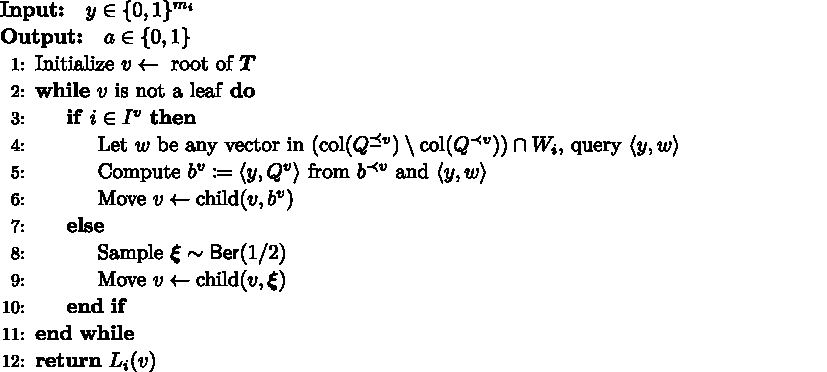
\includegraphics[width=\linewidth,height=0.78\textheight,keepaspectratio]{ccc2025-16-svg-01.pdf}\par




Observe that it is indeed possible to compute the value of $\langle y,Q^{v}\rangle$ from $b^{\prec v}$ and $\langle y,w\rangle$ on line 5: Since $w\notin\mathrm{col}(Q^{\prec v})$, we have $\mathrm{rank}([Q^{\prec v}\>\>w])=\mathrm{rank}(Q^{\prec v})+1$.
On the other hand, as $w\in\mathrm{col}(Q^{\preceq v})$, we have $\mathrm{rank}([Q^{\preceq v}\>\>w])=\mathrm{rank}(Q^{\preceq v})=\mathrm{rank}(Q^{\prec v})+1$. Thus $Q^{v}\in\mathrm{col}([Q^{\prec v}\>\>w])$, which means that $Q^{v}$ can be written as a linear combination of the columns of $[Q^{\prec v}\>\>w]$: $Q^{v}=Q^{u_{1}}+\cdots+Q^{u_{t}}+w$ where $u_{1},\ldots,u_{t}$ are some ancestors of $v$. This in turn implies that $\langle y,Q^{v}\rangle=\sum_{i\in[t]}\langle y,Q^{u_{i}}\rangle+\langle y,w\rangle$.\par




We stress that although $T$ is a deterministic tree, $\mathsf{Ext}_{i}\mathopen{}\left(T\mathclose{}\right)$ is a randomized decision tree with internal randomness inherited from the bits $\bm{\xi}$. Our main technical claim is that for any fixed $y\in\{0,1\}^{m_{i}}$, the algorithm $\mathsf{Ext}_{i}\mathopen{}\left(T\mathclose{}\right)$ perfectly simulates a run of $T$ when the input is on a random input $\bm{x}=(\bm{x}^{1},\ldots,\bm{x}^{i-1},y,\bm{x}^{i+1},\ldots,\bm{x}^{k})$ and $\bm{x}^{j}\sim\mathcal{U}(\{0,1\}^{m_{j}})$. In a nutshell, the randomness of the other $k-1$ instances can be substituted with the internal randomness $\bm{\xi}$. To make this precise, we let $X_{v}=\{x\in\mathcal{X}:x^{T}Q^{\prec v}=b^{\prec v}\}$ be the set of inputs leading to the node $v\in\mathcal{N}(T)$.\par



% SOURCE-ID Thmtheorem22


\par\medskip\noindent\textbf{
Claim 22. 
}\par



For any $y\in\{0,1\}^{m_{i}}$, $\Pr_{\bm{\xi}}[\textup{$\mathsf{Ext}_{i}\mathopen{}\left(T\mathclose{}\right)$ reaches node $v$ in its execution on $y$}]=\Pr_{\bm{x}}[\bm{x}\in X^{v}]$.\par



% END-SOURCE-ID Thmtheorem22



\par\medskip\noindent\textbf{
\textbf{Proof}.}\par




Let us fix $i\coloneqq 1$ and $d\coloneqq d(v)$ for simplicity. We establish and alternative description of $X^{v}$ that puts pure constraints on instance 1 first. Pick $t\coloneqq d_{1}(v)$ independent vectors $Q_{1},\ldots,Q_{t}\in\mathrm{col}(Q^{\prec v})\cap W_{1}$ and extend them arbitrarily to a basis $\{Q_{j}\}_{j\in[d]}$ of $Q^{\prec v}$. As each vector of this basis can be expressed as a linear combination of $\{Q^{u}\}_{u\in\mathrm{path}(v)}$, it is possible to apply those linear combinations to $b^{\prec v}$ and obtain values $\{b_{j}\}_{j\in[d]}$ such that $X_{v}=\{x\in\mathcal{X}\mid\forall j\in[d]:\langle x,Q_{j}\rangle=b_{j}\}$. The set $Y^{v}\subseteq\{0,1\}^{m_{1}}$ of inputs that can reach node $v$ in a run of $\mathsf{Ext}_{1}\mathopen{}\left(T\mathclose{}\right)$ thus corresponds to\par


\[\begin{gathered}
Y^{v}\coloneqq\big{\{}y\in\{0,1\}^{m_{1}}\mid\forall j\in[t]:\langle y,Q_{j}^{1}\rangle=b_{j}\big{\}}.
\end{gathered}\]


If $y\notin Y^{v}$, the statement follows directly as both probabilities are zero. However, if $y\in Y^{v}$,\par


\[\begin{gathered}
\Pr\nolimits_{\bm{\xi}}[\textup{$\mathsf{Ext}_{1}\mathopen{}\left(T\mathclose{}\right)$ reaches node $v$ in its execution}]=2^{-d+t}.
\end{gathered}\]


This is so because a node $v$ can only be reached by having the “right” $d-t$ coin tosses of $\bm{\xi}$ (provided that $y\in Y^{v}$). Thus, it remains to show that $\Pr_{\bm{x}}[\bm{x}\in X^{v}]=2^{-d+t}$ if $y\in Y^{v}$.\par




Let $m=\sum_{i\in[k]}m_{i}$ and $S=\{m_{1}+1,\dots,m\}$ be the indices of the bits of every copy but the first one. Fix the $m\times(d-t)$ boolean matrix $A=[Q_{t+1}\cdots Q_{d}]$ and observe that $\mathrm{rank}(A)=d-t$ by construction. We show that $\mathrm{rank}(A_{S})=d-t$ too. If $\mathrm{rank}(A_{S})<\mathrm{rank}(A)$, we can find a non-empty set $J\subseteq\{t+1,\ldots,d\}$ such that $\sum_{j\in J}(Q_{j})_{S}=0$. This implies that $Q^{\prime}\coloneqq\sum_{j\in J}Q_{j}\in W_{i}\cap\mathrm{col}(Q^{\prec v})$. But $Q^{\prime}$ is linearly independent of $\{Q_{1},\ldots,Q_{t}\}$ – this contradicts $\dim(\mathrm{col}(Q^{\prec v})\cap W_{i})=t$. Therefore, if $y\in Y^{v}$, we use this observation to conclude:\par


\[\begin{gathered}
\displaystyle\Pr\nolimits_{\bm{x}}[\bm{x}\in X^{v}] \displaystyle=\Pr\nolimits_{\bm{x}}[\forall j\in[d]:\langle\bm{x},Q_{j}\rangle=b_{j}] \\
\displaystyle=\Pr\nolimits_{\bm{x}}[\bm{x}^{T}A=(b_{j})_{t+1\leq j\leq d}] \\
\displaystyle=\Pr\nolimits_{\bm{z}\coloneqq(\bm{x}^{2},\dots,\bm{x}^{k})}\left[\bm{z}^{T}A_{S}=(b_{j}+\langle y,Q_{j}^{1}\rangle)_{t+1\leq j\leq d}\right] \\
\displaystyle=2^{-\mathrm{rank}(A_{S})} \\
\displaystyle=2^{-d+t}.\
\end{gathered}\]


$\vartriangleleft$\par






\par\medskip\noindent\textbf{
5.2 Proof of Theorem 18
}\par




We are now ready to show Theorem 18. Let $\mathcal{T}$ be a randomised parity decision tree which witnesses $C\coloneqq{\textup{S}}_{\varepsilon}(f^{k},\mu^{k})$. For each $i\in[k]$, define the randomized decision tree $\mathcal{T}_{i}\colon\{0,1\}^{n}\to\{0,1\}$ with:\par


\begin{enumerate}


\item[] 
1. 


Sample $\bm{T}\sim\mathcal{T}$.\par





\item[] 
2. 


Sample $\bm{\rho}^{1},\,\ldots,\,\bm{\rho}^{i-1},\,\bm{\rho}^{i+1},\,\ldots,\bm{\rho}^{k}\sim\mathcal{R}_{\mu}$.\par





\item[] 
3. 


Let $\widetilde{\bm{\rho}}\coloneqq(\bm{\rho}^{1},\,\ldots,\,\bm{\rho}^{i-1},\,\star^{n},\,\bm{\rho}^{i+1},\,\ldots,\bm{\rho}^{k})$.\par





\item[] 
4. 


Return $\mathsf{Ext}_{i}\mathopen{}\left(T_{\widetilde{\bm{\rho}}}\mathclose{}\right)$.\par





\end{enumerate}


We show in Lemma 23 that $\mathrm{err}_{f}(\mathcal{T}_{i},\mu)\leq\varepsilon$ simultaneously for all $i\in[k]$. On the other hand, we show in Lemma 24 that $\sum_{i\in[k]}\mathop{\overline{sq}}(\mathcal{T}_{i},\mu)\leq C$. By an averaging argument, this shows the existence of a copy $i^{\star}\in[k]$ with cost $\leq C/k$ and therefore ${\textup{S}}_{\varepsilon}(f,\mu)\leq C/k$. The remainder of this section is devoted to proving both claims.\par



% SOURCE-ID Thmtheorem23


\par\medskip\noindent\textbf{
\textbf{Lemma 23}\textbf{.}
}\par



\emph{For every $i\in[k]$, $\mathrm{err}_{f}(\mathcal{T}_{i},\mu)\leq\mathrm{err}_{f^{k}}(\mathcal{T},\mu^{k})$.}\par



% END-SOURCE-ID Thmtheorem23



\par\medskip\noindent\textbf{Proof.}\par




It is enough to prove the statement assuming $\mathcal{T}$ is a deterministic parity tree $T$ and $i=1$. Let $\mathcal{R}$ be the distribution of $\widetilde{\bm{\rho}}$ in the step 3 of generating $\mathcal{T}_{1}$. Fix some $\rho\in\mathrm{supp}(\mathcal{R})$ and note that $\rho^{1}=\star^{n}$. We also define $\mathcal{U}^{-1}\coloneqq\mathcal{U}_{\rho^{2}}\times\cdots\times\mathcal{U}_{\rho^{k}}$. Using Claim 22 on a leaf $\ell\in\mathcal{L}(T_{\rho})$ yields:\par


\[\begin{gathered}
\displaystyle\Pr_{\bm{y},\bm{\xi}}[\textup{$\mathsf{Ext}_{1}\mathopen{}\left(T_{\rho}\mathclose{}\right)$ reaches $\ell$ on $\bm{y}$}\,\wedge\,L_{1}(\ell)\neq f(\bm{y})] \\
\displaystyle= \displaystyle\mathop{\mathbb{E}}_{\bm{y}}\left[\Pr_{\bm{\xi}}[\textup{$\mathsf{Ext}_{1}\mathopen{}\left(T_{\rho}\mathclose{}\right)$ reaches $\ell$ on $\bm{y}$}]\cdot\mathbbm{1}\left[L_{1}(\ell)\neq f(\bm{y})\right]\right] \\
\displaystyle= \displaystyle\mathop{\mathbb{E}}_{\bm{y}}\left[\Pr_{\bm{x}^{-1}\sim\mathcal{U}^{-1}}[(\bm{y},\bm{x}^{-1})\in X^{\ell}]\cdot\mathbbm{1}\left[L_{1}(\ell)\neq f(\bm{y})\right]\right] \\
\displaystyle= \displaystyle\Pr_{\bm{x}\sim\mu\times\mathcal{U}^{-1}}[\bm{x}\in X^{\ell}\,\wedge\,L_{1}(\ell)\neq f(\bm{x}^{1})].
\end{gathered}\]


Thus:\par


\[\begin{gathered}
\displaystyle\mathrm{err}_{f}(\mathcal{T}_{1},\mu) \displaystyle=\mathop{\mathbb{E}}_{\widetilde{\bm{\rho}}\sim\mathcal{R}}\big{[}\Pr\nolimits_{\bm{y}\sim\mu,\,\bm{\xi}}[\mathsf{Ext}_{1}\mathopen{}\left(T_{\widetilde{\bm{\rho}}}\mathclose{}\right)(\bm{y})\neq f(\bm{y})]\big{]} \\
\displaystyle=\mathop{\mathbb{E}}_{\widetilde{\bm{\rho}}}\left[\sum\nolimits_{\ell\in\mathcal{L}(T_{\widetilde{\bm{\rho}}})}\Pr\nolimits_{\bm{x}\sim\mu\times\mathcal{U}^{-1}}\big{[}\bm{x}\in X^{\ell}\,\wedge\,L_{1}(\ell)\neq f(\bm{x}^{1})\big{]}\right] \\
\displaystyle\leq\mathop{\mathbb{E}}_{\widetilde{\bm{\rho}}}\left[\sum\nolimits_{\ell\in\mathcal{L}(T_{\widetilde{\bm{\rho}}})}\Pr\nolimits_{\bm{x}\sim\mu\times\mathcal{U}^{-1}}\big{[}\bm{x}\in X^{\ell}\,\wedge\,L(\ell)\neq f(\bm{x})\big{]}\right] \\
\displaystyle=\mathop{\mathbb{E}}_{\widetilde{\bm{\rho}}}\left[\mathrm{err}_{f^{k}}(T_{\widetilde{\bm{\rho}}},\mu\times\mathcal{U}^{-1})\right].
\end{gathered}\]


Observe now that for any $x\in\mathrm{supp}(\mu\times\mathcal{U}^{-1})$, we have $T_{\widetilde{\bm{\rho}}}(x)=T(x)$. Using the definition of $\mathcal{R}_{\mu}$ thus yields:\par


\[\begin{gathered}
\mathrm{err}_{f}(\mathcal{T}_{1},\mu)\leq\mathop{\mathbb{E}}_{\widetilde{\bm{\rho}}\sim\mathcal{R}}\big{[}\mathrm{err}_{f^{k}}(T_{\bm{\rho}^{-1}},\mu\times\mathcal{U}^{-1})\big{]}=\mathrm{err}_{f^{k}}(T,\mu^{k}).\
\end{gathered}\]


$\blacktriangleleft$\par



% SOURCE-ID Thmtheorem24


\par\medskip\noindent\textbf{
\textbf{Lemma 24}\textbf{.}
}\par



$\sum_{i\in[k]}\mathop{\overline{sq}}(\mathcal{T}_{i},\mu)\leq\mathop{\overline{sq}}(\mathcal{T},\mu^{k})$\emph{.}\par



% END-SOURCE-ID Thmtheorem24




\par\medskip\noindent\textbf{Proof.}\par




It is sufficient to prove this for the case where $\mathcal{T}$ is a deterministic tree $T$. We have:\par


\[\begin{gathered}
\displaystyle\sum\nolimits_{i\in[k]}\mathop{\overline{sq}}(\mathcal{T}_{i},\mu)= \displaystyle\sum\nolimits_{i\in[k]}\mathop{\mathbb{E}}_{\bm{\rho}^{i}\sim\mathcal{R}_{\mu}}\left[\overline{q}((\mathcal{T}_{i})_{\bm{\rho}^{i}},\mathcal{U}_{\bm{\rho}^{i}})\right] \\
\displaystyle= \displaystyle\sum\nolimits_{i\in[k]}\mathop{\mathbb{E}}_{\begin{subarray}{c}\bm{\rho}^{i}\sim\mathcal{R}_{\mu}\\
\widetilde{\bm{\rho}}\sim\mathcal{R}\end{subarray}}\left[\overline{q}\left(\left(\mathsf{Ext}_{i}\mathopen{}\left(T_{\widetilde{\bm{\rho}}}\mathclose{}\right)\right)_{\bm{\rho}^{i}},\mathcal{U}_{\bm{\rho}^{i}}\right)\right] \\
\displaystyle= \displaystyle\sum\nolimits_{i\in[k]}\mathop{\mathbb{E}}_{\bm{\rho}\sim\mathcal{R}_{\mu}^{k}}\left[\overline{q}\left(\mathsf{Ext}_{i}\mathopen{}\left(T_{\bm{\rho}}\mathclose{}\right),\mathcal{U}_{\bm{\rho}^{i}}\right)\right] \\
\displaystyle= \displaystyle\mathop{\mathbb{E}}_{\bm{\rho}\sim\mathcal{R}_{\mu}^{k}}\left[\sum\nolimits_{i\in[k]}\overline{q}\left(\mathsf{Ext}_{i}\mathopen{}\left(T_{\bm{\rho}}\mathclose{}\right),\mathcal{U}_{\bm{\rho}^{i}}\right)\right].
\end{gathered}\]


where the third equality is due to the fact that the operations of applying $\mathsf{Ext}$ and fixing variables are commutable. Let $\rho\in(\{0,\,\star\}^{n})^{k}$ be a partial fixing and $\ell\in\mathcal{L}(T_{\rho})$. The probability that node $\ell$ is visited during the process $\mathsf{Ext}_{i}\mathopen{}\left(T_{\rho}\mathclose{}\right)$ when the input is $\bm{x}^{i}\sim\mathcal{U}_{\rho^{i}}$ is $2^{-d(\ell)}$. Observe that $\mathsf{Ext}_{i}\mathopen{}\left(T_{\rho}\mathclose{}\right)$ only makes $d_{i}(\ell)$ queries to $\bm{x}^{1}$ to reach $\ell$. As such, we have:\par


\[\begin{gathered}
\displaystyle\sum\nolimits_{i\in[k]}\overline{q}\left(\mathsf{Ext}_{i}\mathopen{}\left(T_{\bm{\rho}}\mathclose{}\right),\mathcal{U}_{\bm{\rho}^{i}}\right) \displaystyle=\sum_{i\in[k]}\sum_{\ell\in\mathcal{L}(T^{\prime})}2^{-d(\ell)}d_{i}(\ell) \\
\displaystyle\leq\sum_{\ell\in\mathcal{L}(T^{\prime})}2^{-d(\ell)}d(\ell) \\
\displaystyle=\overline{q}(T_{\rho},\mathcal{U}_{\rho}).
\end{gathered}\]


The inequality is due to the fact that $\sum_{i\in[k]}d_{i}(v)\leq d(v)$. This is because $\dim(W_{i}\cap W_{j})=0$ for each $i\neq j$ and so\par


\[\begin{gathered}
\sum\nolimits_{i\in[k]}d_{i}(v)=\sum\nolimits_{i\in[k]}\dim(\mathrm{col}(Q^{\prec v})\cap W_{i})\leq\dim(\mathrm{col}(Q^{\prec v}))=d(v).
\end{gathered}\]


To conclude, we have\par


\[\begin{gathered}
\sum\nolimits_{i\in[k]}\mathop{\overline{sq}}(\mathcal{T}_{i},\mu)=\mathop{\mathbb{E}}_{\bm{\rho}\sim\mathcal{R}_{\mu}^{k}}\left[\sum\nolimits_{i\in[k]}\overline{q}\left(\mathsf{Ext}_{i}\mathopen{}\left(T_{\bm{\rho}}\mathclose{}\right),\mathcal{U}_{\bm{\rho}^{i}}\right)\right]\leq\mathop{\mathbb{E}}_{\bm{\rho}\sim\mathcal{R}_{\mu}^{k}}\left[\overline{q}(T_{\bm{\rho}},\mathcal{U}_{\bm{\rho}})\right]=\mathop{\overline{sq}}(T,\mu^{k}).\
\end{gathered}\]


$\blacktriangleleft$\par







\par\medskip\noindent\textbf{
6 Direct sum for ${\textup{D}}^{\times}$ part III: from S to ${\textup{D}}^{\times}$
}\par




In this section, we show how to convert parity tree of the ${\textup{S}}_{\varepsilon}$ model to the more common $\overline{{\textup{D}}}_{\varepsilon}$ model and prove Theorems 19 and 20. Let us fix for this section a boolean function $f\colon\{0,1\}^{n}\to\{0,1\}$ together with some $0$-biased product distribution $\mu$ over $\{0,1\}^{n}$. Let $T$ be a deterministic parity tree trying to solve $f$ against $\mu$. We begin by establishing an alternative view of the quantity $\mathop{\overline{sq}}(T,\mu)$. For any fixed $x\in\{0,1\}^{n}$, define the product distribution $R_{\mu}^{x}$ over $\{0,\star\}^{n}$ with:\par


\[\begin{gathered}
\Pr_{\bm{\rho}\sim\mathcal{R}_{\mu}^{x}}[\bm{\rho}_{i}=\star]=\begin{cases}\delta_{i}/(2-\delta_{i})&\quad\textup{if $x_{i}=0$}\\
1&\quad\textup{if $x_{i}=1$}\end{cases}\quad\quad\text{where}\quad\delta_{i}\coloneqq 2\cdot\Pr_{\bm{x}\sim\mu}[\bm{x}_{i}=1]\in[0,1].
\end{gathered}\]


Sampling $\bm{\rho}\sim R_{\mu}$, $\bm{x}\sim\mathcal{U}_{\bm{\rho}}$ and completing $\bm{x}_{j}=0$ for all $\bm{\rho}=0$ is equivalent to first sampling $\bm{x}\sim\mu$ and then some $\bm{\rho}\sim R_{\mu}^{\bm{x}}$. One can therefore see the process of $\mathop{\overline{sq}}(T,\mu)$ as follows:\par


\begin{enumerate}


\item[] 
1. 


Sample $\bm{x}\sim\mu$, $\bm{\rho}\sim R_{\mu}^{\bm{x}}$.\par





\item[] 
2. 


Run $T$ on $\bm{x}$.\par





\item[] 
3. 


Every time $T$ attempts to make a query, check if $\bm{\rho}$ simplifies the query: $\bm{\rho}_{i}=0\implies\bm{x}_{i}=0$.\par





\end{enumerate}


We describe this alternative view in detail in Algorithm 2. With this new interpretation, we can recast the quantity $\mathop{\overline{sq}}(T,\mu)$ with\par


\[\begin{gathered}
\mathop{\overline{sq}}(T,\mu)=\mathop{\mathbb{E}}\nolimits_{\bm{x}\sim\mu,\bm{\rho}\sim R_{\mu}^{\bm{x}}}[\text{Number of times
line\nobreak\ 4 is executed in Algorithm 2}].
\end{gathered}\]


The idea to convert ${\textup{S}}_{\varepsilon}$ algorithms to $\overline{{\textup{D}}}_{\varepsilon}$ ones is to simulate the process of Algorithm 2 by maintaining an incomplete but consistent view $p\in\{0,\star,\mathord{?}\}^{n}$ of $\rho$. Initially, $p=\mathord{?}^{n}$ – i.e. nothing is known about $\rho$ – and we gradually update $p$ based on the queries we get. For instance, if $x_{i}=1$, then ˜3 asserts $\rho_{i}=\star$. This scheme helps to relate the cost of the converted $\overline{{\textup{D}}}_{\varepsilon}$ algorithm with $\mathop{\overline{sq}}(T,\mu)$. The description of the converted algorithm is given in Algorithm 3.\par


\textbf{Algorithm 2}  an alternative view of $\mathop{\overline{sq}}(T,\mu)$.
\par\noindent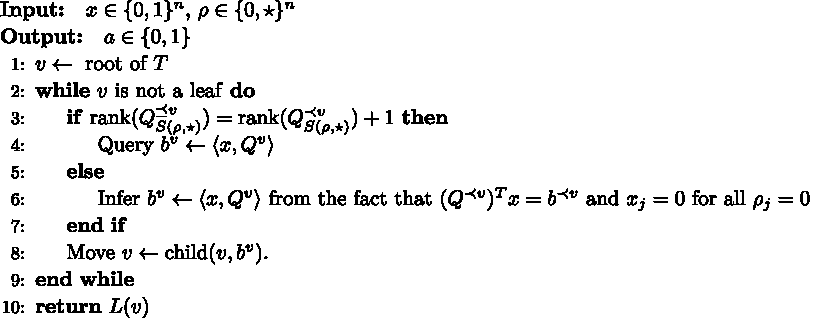
\includegraphics[width=\linewidth,height=0.78\textheight,keepaspectratio]{ccc2025-16-svg-02.pdf}\par


\textbf{Algorithm 3}  converts an algorithm $T$ for ${\textup{S}}_{\varepsilon}$ to $\overline{{\textup{D}}}_{\varepsilon}$.
\par\noindent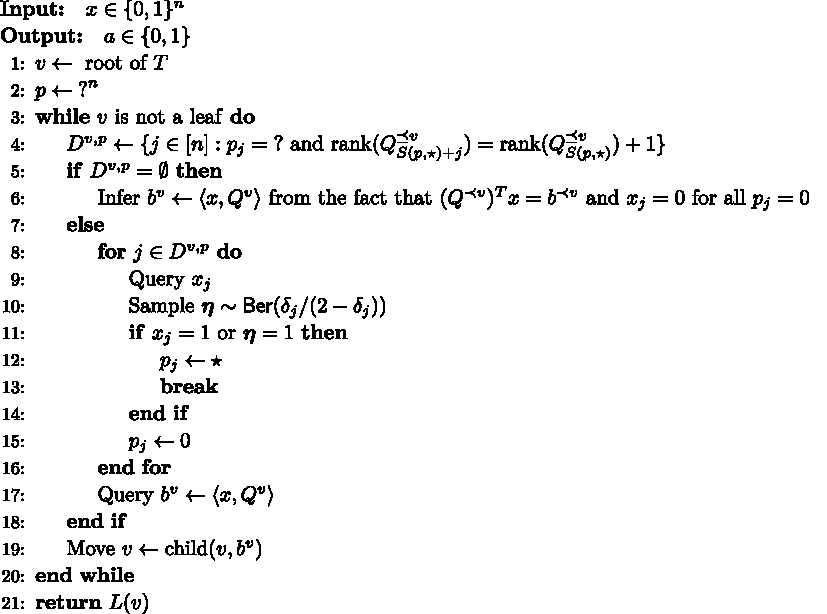
\includegraphics[width=\linewidth,height=0.78\textheight,keepaspectratio]{ccc2025-16-svg-03.pdf}\par



% SOURCE-ID Thmtheorem25


\par\medskip\noindent\textbf{
\textbf{Definition 25}\textbf{.}
}\par



\emph{Let $p\in\{0,\star,\mathord{?}\}^{n}$ be a fixing. The following are subsets of indices:}\par


\[\begin{gathered}
S^{p}_{\star}=\{j\in[n]:p_{j}=\star\}\quad S^{p}_{0}=\{j\in[n]:p_{j}=0\}\quad S^{p}_{\mathord{?}}=\{j\in[n]:p_{j}=\mathord{?}\}\quad S^{p}_{\neq 0}=S^{p}_{\star}\cup S^{p}_{\mathord{?}}
\end{gathered}\]


\emph{We also write $S(p,\star)$ to mean $S^{p}_{\star}$ and likewise for other sets.}\par



% END-SOURCE-ID Thmtheorem25



Let $P^{v}\subseteq\{0,\star,\mathord{?}\}^{n}$ be the set of all possible $p$ that could be at the start of an iteration of Algorithm 3 at node $v$. We now prove an invariant of Algorithm 3 and then its correctness.\par



% SOURCE-ID Thmtheorem26


\par\medskip\noindent\textbf{
\textbf{Lemma 26}\textbf{.}
}\par



\emph{For any state $v\in\mathcal{N}(T)$ and $p\in P^{v}$ that Algorithm 3 could be in at the start of a while iteration (line 3), it holds that:}\par


\[\begin{gathered}
\mathrm{rank}\Big{(}Q^{\prec v}_{S(p,\neq 0)}\Big{)}=\mathrm{rank}\Big{(}Q^{\prec v}_{S(p,\star)}\Big{)}=|S(p,\star)|.
\end{gathered}\]



% END-SOURCE-ID Thmtheorem26



\par\medskip\noindent\textbf{Proof.}\par




We prove the claim by induction on $T$. The statement is true when $v$ is the root because both $Q^{\prec v}$ and $S^{p}_{\star}$ are empty. Let us now assume that the statement is true for some $v$ and $p\in P^{v}$ and prove that the invariant carries over to the next iteration regardless of the query outcomes and the randomness $\bm{\eta}$ of the process. If $p^{\prime}$ is the updated value of $p$ at line 19, this amounts to showing that $\mathrm{rank}(Q^{\preceq v}_{S(p^{\prime},\neq 0)})=\mathrm{rank}(Q^{\preceq v}_{S(p^{\prime},\star)})=|S(p^{\prime},\star)|$. We consider three cases.\par





\par\medskip\noindent\textbf{Case $D^{v,p}=\emptyset$.}\par




Then, there is no update for $p$ and $p^{\prime}=p$. Since $\mathrm{rank}(Q^{\preceq v}_{S(p,\star)})=\mathrm{rank}(Q^{\preceq v}_{S(p,\star)+j})$ for all $j\in S(p,\neq 0)$, we have $\mathrm{rank}(Q^{\preceq v}_{S(p,\neq 0)})=\mathrm{rank}(Q^{\preceq v}_{S(p,\star)})=|S(p,\star)|$, as desired.\par





\par\medskip\noindent\textbf{Case $D^{v,p}\neq\emptyset$ and $p^{\prime}_{j}=0$ for all $j\in D^{v,p}$.}\par




Then, $S^{p^{\prime}}_{\star}=S^{p}_{\star}$ and $S(p^{\prime},\neq 0)=S(p,\neq 0)\setminus D^{v,p}$. By definition of $D^{v,p}$, we still have $\mathrm{rank}(Q^{\preceq v}_{S(p,\star)})=\mathrm{rank}(Q^{\preceq v}_{S(p,\star)+j})$ for all $j\in S(p^{\prime},\neq 0)$, so $\mathrm{rank}(Q^{\preceq v}_{S(p^{\prime},\neq 0)})=\mathrm{rank}(Q^{\preceq v}_{S(p^{\prime},\star)})=|S(p^{\prime},\star)|$.\par





\par\medskip\noindent\textbf{Case $D^{v,p}\neq\emptyset$ and $p^{\prime}_{j}=\star$ for some $j\in D^{v,p}$.}\par




Then $S^{p^{\prime}}_{\star}=S_{\star}^{p}+j$ and it must hold that $\mathrm{rank}(Q^{\preceq v}_{S(p^{\prime},\star)})=|S(p^{\prime},\star)|$. On the other hand,\par


\[\begin{gathered}
\mathrm{rank}\Big{(}Q^{\preceq v}_{S(p^{\prime},\neq 0)}\Big{)}\leq\mathrm{rank}\Big{(}Q^{\prec v}_{S(p,\neq 0)}\Big{)}+1=|S(p,\star)|+1=|S(p^{\prime},\star)|.
\end{gathered}\]


Where the inequality follows from the fact that $S(p^{\prime},\neq 0)\subseteq S(p,\neq 0)$. Finally, this implies $\mathrm{rank}(Q^{\preceq v}_{S(p^{\prime},\neq 0)})=\mathrm{rank}(Q^{\preceq v}_{S(p^{\prime},\star)})=|S(p,\star)|$.
$\blacktriangleleft$\par



% SOURCE-ID Thmtheorem27


\par\medskip\noindent\textbf{
\textbf{Lemma 27}\textbf{.}
}\par



\emph{For any $x\in\{0,1\}^{n}$, $\Pr_{\bm{\eta}}[\textup{Algorithm 3 outputs $1$}]=\mathbbm{1}\left[T(x)=1\right]$.}\par



% END-SOURCE-ID Thmtheorem27




\par\medskip\noindent\textbf{Proof.}\par




It is not hard to see that if Algorithm 3 gets the correct value of $\langle x,Q^{v}\rangle$ at each iteration of the while loop, it perfectly simulates $T$. Thus, it suffices to show that whenever $D^{v,p}=\emptyset$, the algorithm can compute the value of $\langle x,Q^{v}\rangle$ from the previous query outcomes. Lemma 26 and its proof implies that if $D^{v,p}=\emptyset$, then $\mathrm{rank}(Q^{\preceq v}_{S(p,\neq 0)})=\mathrm{rank}(Q^{\prec v}_{S(p,\neq
0)})=|S(p,\star)|$. Thus $Q^{v}_{S(p,\neq 0)}$ can be written as a linear combination of column vectors of $Q^{\prec v}_{S(p,\neq 0)}$. Namely, $Q^{v}_{S(p,\neq 0)}=\sum_{j\in[t]}Q^{v_{j}}_{S(p,\neq 0)}$, where $v_{1},\ldots,v_{t}$ are some ancestors of $v$. On the other hand, we know that $x_{j}=p_{j}=0$ for all $j\in S^{p}_{0}$. Consequently, we have\par


\[\begin{gathered}
\langle x,Q^{v}\rangle=\langle x,Q^{v}\rangle_{S(p,\neq 0)}=\sum\nolimits_{j\in[t]}\langle x,Q^{v_{j}}\rangle_{S(p,\neq 0)}=\sum\nolimits_{j\in[t]}b^{v_{j}}.
\end{gathered}\]


Thus, Algorithm 3 follows the same path of vertices as $T$, irrespective of the randomness $\bm{\eta}$. Consequently, its outputs correspond to the one of $T$.
$\blacktriangleleft$
We now turn our attention to the efficiency of Algorithm 3. We shall start with the special case of $\mu$ being a constant-bounded distribution. In this particular case, we obtain a lossless conversion.
We then turn our attention to general product distributions, for which Algorithm 3 suffers a $\log(n)$ factor. This loss factor is inherent to reducing ${\textup{S}}_{\varepsilon}$ to $\overline{{\textup{D}}}$ as Section 8 shows.\par





\par\medskip\noindent\textbf{
6.1 Conversion for constant-bounded distribution}\par




We now prove a strong efficiency result for Algorithm 3 in the special case where $\mu$ is $\lambda$-bounded (see Definition 13). A proof of our goal (Theorem 20) then follows easily.\par



% SOURCE-ID Thmtheorem28


\par\medskip\noindent\textbf{
\textbf{Lemma 28}\textbf{.}
}\par



\emph{We have $\overline{q}(\textup{Algorithm 3 on $T$},\mu)\leq(2/\lambda)\cdot\mathop{\overline{sq}}(T,\mu)$.}\par



% END-SOURCE-ID Thmtheorem28



Before proving this, we need an alternative view of the randomness used in the for-loop of Algorithm 3 (line 8 to 16). At the start of the process, a random partial fixing $\bm{\rho}\sim\mathcal{R}_{\mu}^{x}$ is generated. The algorithm is then deterministic: whenever some $x_{j}$ is queried in the for-loop, this is replaced by a query to $\bm{\rho}_{j}$. The algorithm updates $p_{j}$ with $\bm{\rho}_{j}$ and exits the loop if $\bm{\rho}_{j}=\star$. This process is given in detail in Algorithm 4.\par


\textbf{Algorithm 4}  an alternative view of Algorithm 3 where the randomness is fixed at the start.
\par\noindent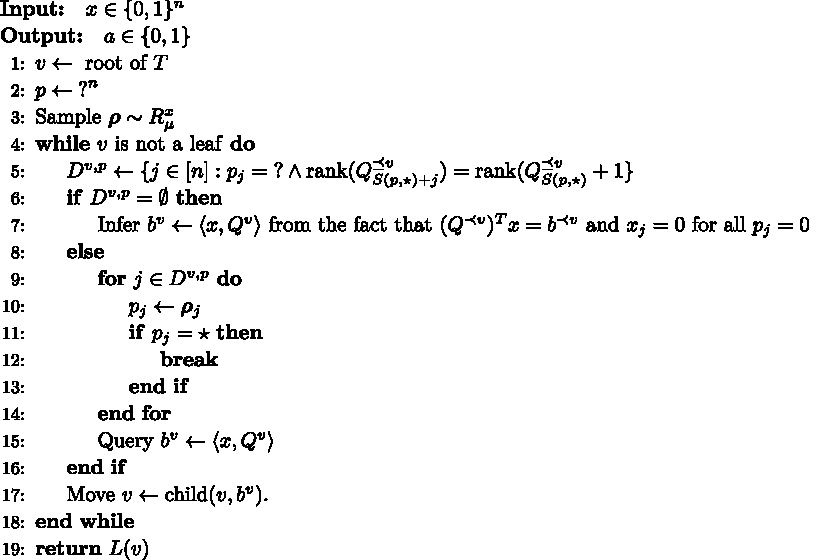
\includegraphics[width=\linewidth,height=0.78\textheight,keepaspectratio]{ccc2025-16-svg-04.pdf}\par




Note that as $R^{x}_{\mu}$ is a product distribution, one can actually implement Algorithm 4 without querying all of $x$ at the start. Indeed, it is enough to query $x_{j}$ whenever one needs the value of $\bm{\rho}_{j}$, similarly to Algorithm 3. This implies that both processes are equivalent.\par




Suppose one runs Algorithm 4 on $\bm{x}\sim\mu$ and $\bm{\rho}\sim R^{\bm{x}}_{\mu}$. Fix some state $(v,p)$ the algorithm could be in at the start of the while loop (line 5). We let $\mathcal{X}^{v,p}$ be the distribution of $\bm{x}$ conditioned on reaching state $(v,p)$. Furthermore, for a fixed $x\in\{0,1\}^{n}$ and $(v,p)$ reachable with $x$ we let $\mathcal{R}^{v,p,x}$ be the marginal distribution of $\bm{\rho}$ conditioned on reaching state $(v,p)$ and $\bm{x}=x$. We now develop explicit formulations for those distributions.\par




\par\medskip\noindent\textbf{Explicit definition of $\mathcal{X}^{v,p}$
}\par




Let $\widehat{\mathcal{X}}^{v,p}$ be the distribution over $\{0,1\}^{n}$ defined as follows:\par


\begin{enumerate}


\item[] 
1. 


For all $j\in S^{p}_{0}$, fix $\bm{x}_{j}=0$.\par





\item[] 
2. 


For all $j\in S^{p}_{\mathord{?}}$, sample $\bm{x}_{j}\sim\mathsf{Ber}(\delta_{j}/2)$.\par





\item[] 
3. 


Determine $\{\bm{x}_{j}\colon j\in S^{p}_{\star}\}$ by solving $\left\{\langle x,Q^{u}\rangle_{S(p,\star)}=\langle x,Q^{u}\rangle_{S(p,\neq\star)}+b^{u}\right\}_{u\in\mathrm{path}(v)}$\par





\end{enumerate}





\par\medskip\noindent\textbf{Explicit definition of $\mathcal{R}^{v,p,x}$
}\par




Let $\widehat{\mathcal{R}}^{p,x}$ be the product distribution over $\{0,\star\}^{n}$ defined as follows:\par


\begin{enumerate}


\item[] 
1. 


For all $j\in S^{p}_{\mathord{?}}$ such that $x_{j}=0$, let $\bm{\rho}_{j}=*$ with probability $\delta_{j}/(2-\delta_{j})$ and $\bm{\rho}_{j}=0$ else.\par





\item[] 
2. 


For all $j\in S^{p}_{\mathord{?}}$ such that $x_{j}=1$, fix $\bm{\rho}_{j}=\star$.\par





\item[] 
3. 


For all $j\in S(p,\neq\mathord{?})$, fix $\bm{\rho}_{j}=p_{j}$.\par





\end{enumerate}



% SOURCE-ID Thmtheorem29


\par\medskip\noindent\textbf{
Claim 29. 
}\par



For every reachable state $(v,p)$ and $x\in\mathrm{supp}(\mathcal{X}^{v,p})$ in Algorithm 4, we have\par


\begin{enumerate}


\item[] 
1. 


$\mathcal{R}^{v,p,x}\equiv\widehat{\mathcal{R}}^{p,x}$;\par





\item[] 
2. 


$\mathcal{X}^{v,p}\equiv\widehat{\mathcal{X}}^{v,p}$.\par





\end{enumerate}



% END-SOURCE-ID Thmtheorem29



We delay the proof of this technical lemma to Section A.5. We can now prove the efficiency of our algorithm for $\lambda$-bounded distributions.\par




\par\medskip\noindent\textbf{Proof of Lemma 28.}\par




To relate Algorithm 2 with Algorithm 4, it is helpful to insert the book-keeping of $p$ in Algorithm 2 (lines 5 to 16, without 10) in between Algorithms 2 and 4 of Algorithm 2. This doesn’t change the number of queries or guarantees of Algorithm 2 but now both processes share the same state space over $(v,p)$. For $x\in\{0,1\}^{n}$ and $\rho\in\{0,\star\}^{n}$, define $A(x,\rho)$ and $B(x,\rho)$ as the number of queries each process makes:\par




\[\begin{gathered}
\displaystyle A(x,\rho) \displaystyle\coloneqq\text{number of times line\nobreak\ 4 is executed in Algorithm 2 on input $(x,\rho)$}; \\
\displaystyle B(x,\rho) \displaystyle\coloneqq\text{number of times Algorithms 4 and\nobreakspace4 are executed in Algorithm 4 on input $(x,\rho)$}.
\end{gathered}\]


Using ˜4, it is thus enough to prove that $\mathop{\mathbb{E}}_{\bm{x},\bm{\rho}}\left[A(\bm{x},\bm{\rho})\right]\geq\Omega(\lambda)\cdot\mathop{\mathbb{E}}_{\bm{x},\bm{\rho}}\left[B(\bm{x},\bm{\rho})\right]$ when $\bm{x}\sim\mu$ and $\bm{\rho}\sim R_{\mu}^{\bm{x}}$. We have:\par


\[\begin{gathered}
\mathop{\mathbb{E}}_{\bm{x},\bm{\rho}}[A(\bm{x},\bm{\rho})]=\sum_{(v,p)}\Pr_{\bm{x},\bm{\rho}}[\text{$(v,p)$ is reached}]\cdot\Pr_{\begin{subarray}{c}\bm{x}\sim\mathcal{X}^{v,p}\\
\bm{\rho}\sim\mathcal{R}^{v,p,\bm{x}}\end{subarray}}\Big{[}\mathrm{rank}(Q^{\preceq v}_{S(\bm{\rho},\neq 0)})=\mathrm{rank}(Q^{\prec v}_{S(\bm{\rho},\neq 0)})+1\Big{]}.
\end{gathered}\]


As both algorithms follow the same path in the state space, this expectation can be computed with respect to the code of Algorithm 4. Fix some state $(v,p)$ and observe that if there exists some $j\in D^{v,p}$ such that $\bm{\rho}_{j}=\star$, then by Lemma 26,\par


\[\begin{gathered}
\mathrm{rank}(Q^{\preceq v}_{S({\bm{\rho}},\neq)})=\mathrm{rank}(Q^{\preceq v}_{S(p,\star)+j})=\mathrm{rank}(Q^{\prec v}_{S(p,\star)})+1=\mathrm{rank}(Q^{\prec v}_{S(\bm{\rho},\neq 0)})+1.
\end{gathered}\]


Therefore, for $\bm{x}\sim\mathcal{X}^{v,p}$ and $\bm{\rho}\sim\mathcal{R}^{v,p,\bm{x}}$, we have\par


\[\begin{gathered}
\displaystyle\Pr\nolimits_{\bm{x},\bm{\rho}}\Big{[}\mathrm{rank}(Q^{\preceq v}_{S(\bm{\rho},\neq 0)})=\mathrm{rank}(Q^{\prec v}_{S(\bm{\rho},\neq 0)})+1\Big{]} \displaystyle\geq\Pr\nolimits_{\bm{x},\bm{\rho}}\left[\exists j\in D^{v,p}:\bm{\rho}_{j}=\star\right] \\
\displaystyle=1-\Pr\nolimits_{\bm{x},\bm{\rho}}[\forall j\in D^{v,p}:\bm{\rho}_{j}=\bm{x}_{j}=0].
\end{gathered}\]


The last equality is due to the fact that for all $j\in D^{v,p}$, if $\bm{\rho}_{j}=0$ then $\bm{x}_{j}=0$. Let $D\coloneqq D^{v,p}$. We can now substitute $\widehat{\mathcal{X}}^{v,p}$ for $\mathcal{X}^{v,p}$ and $\widehat{\mathcal{R}}^{p,\bm{x}}$ for $\mathcal{R}^{v,p,\bm{x}}$ using Claim 29:\par


\[\begin{gathered}
\displaystyle\Pr_{\bm{x},\bm{\rho}}[\forall j\in D\colon\bm{\rho}_{j}=\star\land\bm{x}_{j}=0] \\
\displaystyle= \displaystyle\Pr_{\bm{x},\bm{\rho}}[\forall j\in D\colon\bm{x}_{j}=0]\cdot\Pr_{\bm{x},\bm{\rho}}[\forall j\in D\colon\bm{\rho}_{j}=\star\mid\forall j\in D\colon\bm{x}_{j}=0] \\
\displaystyle= \displaystyle\prod\nolimits_{j\in D}(1-\delta_{j}/2)\cdot\prod\nolimits_{j\in D}\frac{2-2\delta_{j}}{2-\delta_{j}} \\
\displaystyle= \displaystyle\prod\nolimits_{j\in D}(1-\delta_{j}) \\
\displaystyle\leq \displaystyle(1-\lambda)^{|D|}.
\end{gathered}\]


Thus, if $\bm{x}\sim\mu$ and $\bm{\rho}\sim R_{\mu}^{\bm{x}}$, we have\par


\[\begin{gathered}
\mathop{\mathbb{E}}_{\bm{x},\bm{\rho}}[A(\bm{x},\bm{\rho})]\geq\sum\nolimits_{(v,p)}\Pr\nolimits_{\bm{x},\bm{\rho}}[\text{state $(v,p)$ is reached}]\cdot\Big{(}1-(1-\lambda)^{|D^{v,p}|}\Big{)}.
\end{gathered}\]


We now bound the expected number of queries made by $\mathcal{T}$. When $D^{v,p}=\emptyset$, $\mathcal{T}$ skips making a query at $v$. On the other hand, when $D^{v,p}\neq\emptyset$, the algorithm goes over $j\in D^{v,p}$ and stops making queries as soon as it hits some $\rho_{j}=\star$. This probability is independent for each $j\in D^{v,p}$ and can be computed explicitly using Claim 29. For $\bm{x}\sim\mathcal{X}^{v,p}$ and $\bm{\rho}\sim\mathcal{R}^{v,p,x}$:\par


\[\begin{gathered}
\Pr_{\bm{x},\bm{\rho}}[\bm{\rho}_{j}=*]=\Pr_{\bm{x}}[\bm{x}_{j}=0]\cdot\Pr_{\bm{x},\bm{\rho}}[\rho_{j}=\star\mid\bm{x}_{j}=0]+\Pr_{\bm{x}}[\bm{x}_{j}=1]\cdot\Pr_{\bm{x}}[\bm{\rho}_{j}=\star\mid\bm{x}_{j}=1]=\delta_{j}\geq\lambda.
\end{gathered}\]


Therefore, if $\bm{x}\sim\mu$ and $\bm{\rho}\sim R_{\mu}^{\bm{x}}$,\par


\[\begin{gathered}
\displaystyle\mathop{\mathbb{E}}_{\bm{x},\bm{\rho}}[B(\bm{x},\bm{\rho})] \\
\displaystyle\leq \displaystyle\sum\nolimits_{(v,p)}\Pr_{\bm{x},\bm{\rho}}[\text{state $(v,p)$ is reached}]\cdot\left(\mathbbm{1}\left[D^{v,p}\neq\emptyset\right]+\sum\nolimits_{j=0}^{|D^{v,p}|-1}(1-\lambda)^{j}\right) \\
\displaystyle\leq \displaystyle\sum\nolimits_{(v,p)}\Pr_{\bm{x},\bm{\rho}}[\text{state $(v,p)$ is reached}]\cdot\left(\mathbbm{1}\left[D^{v,p}\neq\emptyset\right]+\Big{(}1-(1-\lambda)^{|D^{v,p}|}\Big{)}/\lambda\right) \\
\displaystyle\leq \displaystyle\sum\nolimits_{(v,p)}\Pr_{\bm{x},\bm{\rho}}[\text{state $(v,p)$ is reached}]\cdot\left(2/\lambda\right)\cdot\Big{(}1-(1-\lambda)^{|D^{v,p}|}\Big{)}.\
\end{gathered}\]


$\blacktriangleleft$
With this in hand, we can now prove Theorem 20, which we restate below for convenience.
See 20\par





\par\medskip\noindent\textbf{Proof.}\par




Let $\mathcal{T}$ be a randomised parity tree such that $\mathop{\overline{sq}}(\mathcal{T},\mu)={\textup{S}}_{\varepsilon}(f,\mu)$ and $\mathrm{err}_{f}(\mathcal{T},\mu)\leq\varepsilon$. Define $\mathcal{T}^{\prime}$ to be the randomised algorithm obtained by sampling $\bm{T}\sim\mathcal{T}$ and returning Algorithm 3 applied to $\bm{T}$. Using Lemma 27, we immediately obtain that $\mathrm{err}(\mathcal{T}^{\prime},\mu)\leq\varepsilon$. On the other hand:\par


\[\begin{gathered}
\overline{q}(\mathcal{T}^{\prime},\mu)=\mathop{\mathbb{E}}_{\bm{T}}\big{[}\overline{q}(\text{Algorithm 3 on $\bm{T}$},\mu)\big{]}\leq(2/\lambda)\cdot\mathop{\mathbb{E}}_{\bm{T}}[\mathop{\overline{sq}}(\bm{T},\mu)]=(2/\lambda)\cdot{\textup{S}}_{\varepsilon}(f,\mu).
\end{gathered}\]


Thus, $\overline{{\textup{D}}}_{\varepsilon}(f,\mu)\leq O(1/\lambda)\cdot{\textup{S}}_{\varepsilon}(f,\mu)$, as desired.
$\blacktriangleleft$\par







\par\medskip\noindent\textbf{
6.2 Conversion for general product distribution}\par




Algorithm 3 is not efficient for arbitrary product distribution since queries can be very biased so that $\prod_{j\in D^{v,p}}(1-\delta_{j})=1-o(1)$. In such cases, we cannot even afford to pay one query as the corresponding expected increment for $\mathop{\overline{sq}}$ is $o(1)$.\par




To overcome this obstacle, we introduce the following idea. Run the algorithm as if every query $x_{j}$ returned $0$, i.e. assuming $x_{j}=\bm{\rho}_{j}=0$ for all $j\in S(p,\mathord{?})$ (this is likely to happen for very biased distributions). This generates a list of indices for which we assume $x_{j}=0$. Upon reaching a leaf, we check efficiently whether one of those $x_{j}$ is actually $1$. If no such $j$ exists, we’re done – at the cost of \emph{no real} queries! On the other hand, if a $1$ is found, we backtrack to this state and restart the procedure. Since we’ve found $x_{j}=1$, it must be that $\rho_{j}=\star$ and the ${\textup{S}}_{\varepsilon}$ algorithm has to pay one query there.\par




The process $\mathsf{BuildList}$ that “runs assuming $x_{j}=0$” and produces a list of indices to check is described in Algorithm 6. Then, the updated algorithm for converting an ${\textup{S}}_{\varepsilon}$ algorithm to a $\overline{{\textup{D}}}_{\varepsilon}$ one is formulated in Algorithm 5.\par


\textbf{Algorithm 5}  converts an algorithm for ${\textup{S}}_{\varepsilon}$ to $\overline{{\textup{D}}}_{\varepsilon}$ for general product distributions.
\par\noindent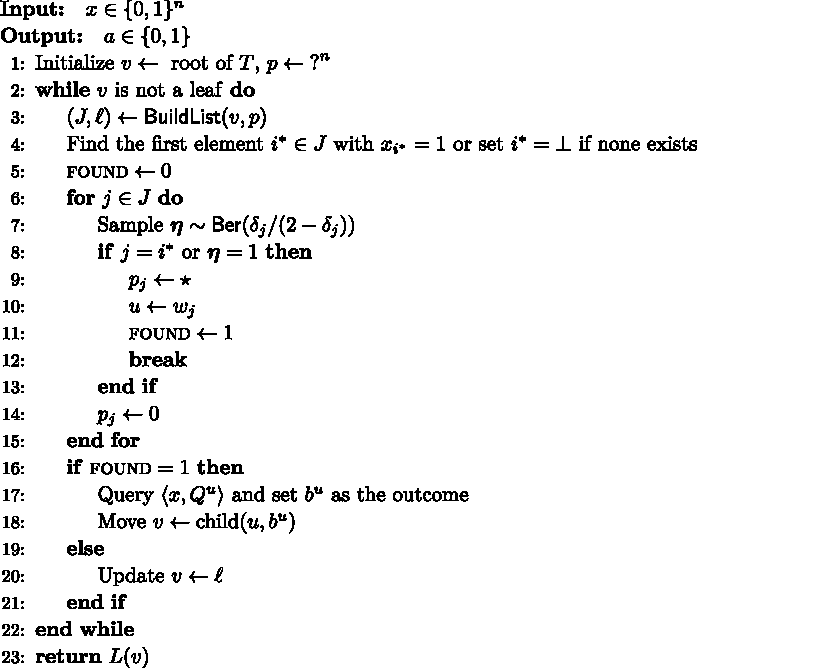
\includegraphics[width=\linewidth,height=0.78\textheight,keepaspectratio]{ccc2025-16-svg-05.pdf}\par


\textbf{Algorithm 6}  the subroutine $\mathsf{BuildList}$.
\par\noindent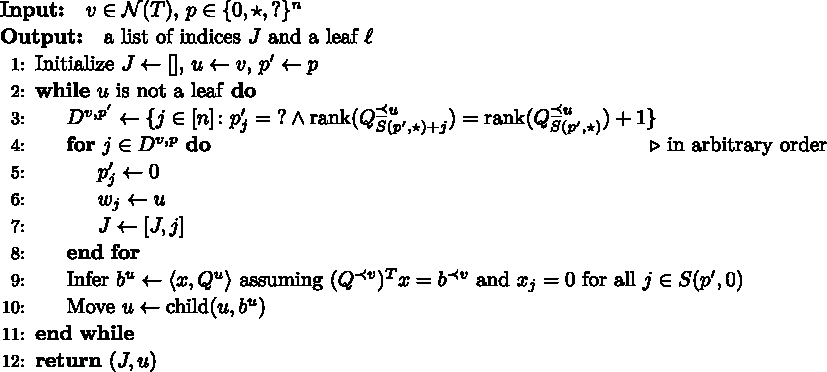
\includegraphics[width=\linewidth,height=0.78\textheight,keepaspectratio]{ccc2025-16-svg-06.pdf}\par




\par\medskip\noindent\textbf{How to run line 4?}\par




This problem can be formulated as follows. Let ${\textrm{\small{FFO}}}_{n}:\{0,1\}^{n}\to[n]\cup\bot$ be the search problem that asks for the index of the first (running from left to right) ’1’ in $x$ or $\bot$ if $x=0^{n}$. Even though a simple adversary argument shows that one cannot perfectly compute ${\textrm{\small{FFO}}}_{n}$ by making $<n$ parity queries, a folklore result [24, 44, 30], proves that there is a randomised protocol making $O(\log n)$ queries that computes ${\textrm{\small{FFO}}}_{n}$ with some small error.\par



% SOURCE-ID Thmtheorem30


\par\medskip\noindent\textbf{
\textbf{Lemma 30}\textbf{.}
}\par



\emph{For any $\alpha>0$, ${\textup{R}}_{\alpha}(\textup{{{\small{FFO}}}}_{n})\leq O\big{(}\log n+\log(1/\alpha)\big{)}$.}\par



% END-SOURCE-ID Thmtheorem30



\par\medskip\noindent\textbf{Proof.}\par




This folklore fact is discussed for the parity context in Section A.4.
$\blacktriangleleft$
We let $\mathcal{T}^{\prime}_{\gamma}$ be the parity tree obtained by running Algorithm 5 with error parameter $\alpha\coloneqq\gamma/n$ on line 4. Given two indices $i,j\in J$, we say $i\prec_{J}j$ if $i$ appears strictly earlier than $j$ in $J$, and $i\preceq_{J}j$ if $i\prec_{J}j$ or $i=j$. Fix any $x\in\mathrm{supp}(\mathcal{X}^{v,p})$. Let $i^{*}$ denote the first index $i$ in $J$ such that $x_{i}=1$ and suppose that $i^{*}$ is added to $J$ when $u=u^{*}$. Observe that if such $i^{*}$ exists, $x_{j}=0$ for all $j\prec_{J}i^{*}$. As a consequence, we know that $u^{*}$ must be reached. Moreover, we can immediately get the values of $\bm{\rho}_{j}$ by flipping biased coins for all $j\preceq_{J}i^{*}$. Therefore, given $i^{*}$, one can perfectly simulate Algorithm 3 by going over $J$ and updating $p$, until finding the first index $j^{*}\preceq_{J}i^{*}$ such that $\bm{\rho}_{j^{*}}=\star$. We are now ready to prove the correctness and efficiency of $\mathcal{T}^{\prime}_{\gamma}$.\par



% SOURCE-ID Thmtheorem31


\par\medskip\noindent\textbf{
\textbf{Lemma 31}\textbf{.}
}\par



\emph{For any fixed $x\in\{0,1\}^{n}$, $\Pr[\mathcal{T}^{\prime}_{\gamma}(x)=1]\in\mathbbm{1}\left[T(x)=1\right]\pm\gamma$.}\par



% END-SOURCE-ID Thmtheorem31




\par\medskip\noindent\textbf{Proof.}\par




The randomness of $\mathcal{T}^{\prime}_{\gamma}$ stems from $\bm{\eta}$ and the randomness involved in running the FFO algorithm at line 4. To analyse the latter, observe that line 4 is called at most $n$ times and each call fails with probability at most $\alpha=\gamma/n$, hence:\par


\[\begin{gathered}
d_{\mathrm{TV}}(\mathcal{T}^{\prime}_{0}(x),\mathcal{T}^{\prime}_{\gamma}(x))\leq\Pr[\text{at least one oracle call at line\nobreak\ 4 gives a wrong index}]\leq n\cdot\frac{\gamma}{n}=\gamma.
\end{gathered}\]


If no call fails the discussion above implies that Algorithm 5 behaves identically to the earlier Algorithm 3. Hence, correctness of the former (Lemma 27) implies $\Pr[\mathcal{T}^{\prime}_{0}(x)=1]=\mathbbm{1}\left[T(x)=1\right]$.
$\blacktriangleleft$\par



% SOURCE-ID Thmtheorem32


\par\medskip\noindent\textbf{
\textbf{Lemma 32}\textbf{.}
}\par



\emph{We have $\overline{q}(\mathcal{T}^{\prime}_{\gamma},\mu)\leq O(\log(n/\gamma))\cdot(\mathop{\overline{sq}}(T,\mu)+1)+\gamma\cdot n$.}\par



% END-SOURCE-ID Thmtheorem32




\par\medskip\noindent\textbf{Proof.}\par




We first prove that the expected number of iterations of the outer while-loop is low assuming that the algorithm always gets the correct index $i^{*}$ at line 4. Similar to what we did in Section 6.1, we view the randomness used in the for-loop (line 6 to 15) in Algorithm 5 as a pre-generated partial assignment $\bm{\rho}\sim\mathcal{R}_{\mu}^{x}$. Note that the bits of $\bm{\rho}$ are independent. If $i^{*}$ is the first index in $J$ with $x_{i^{*}}=1$, we know that $x_{i^{*}}=1$ and $x_{j}=0$ for all $j\prec_{J}i^{*}$. At the same time, $\bm{\rho}_{j}$ for all $j\preceq_{J}i$ are revealed to the algorithm one by one. As soon as some $\bm{\rho}_{j}=\star$ is found, the algorithm quits the loop.\par




For each $x\in\{0,1\}^{n}$ and $\rho\in\mathrm{supp}(\mathcal{R}_{\mu}^{x})$, consider running $\mathcal{T}^{\prime}_{\gamma}$ on input $x$ using randomness $\rho$.
Define $K(x,\rho)$ as the number of iterations of the outer while loop when $\mathcal{T}^{\prime}_{\gamma}$ always gets the correct $i^{*}$ on line 4. Let $p^{*}$ denote the final state of $p$. Since in each iteration except for the last one, we update some $p_{j}$ as $\star$, we have $K(x,\rho)\leq|S(p^{*},\star)|+1$. By Lemma 26, we further have\par


\[\begin{gathered}
K(x,\rho)\leq\mathrm{rank}\left(Q^{\prec\ell(x)}_{S(p^{*},\star)}\right)+1=\mathrm{rank}\left(Q^{\prec\ell(x)}_{S(p^{*},\neq 0)}\right)+1,
\end{gathered}\]


where $\ell(x)\in\mathcal{L}(T)$ is the unique leaf at which $T$ terminates given $x$. Since for all $p_{j}\neq?$, $p_{j}=\rho_{j}$, we have $S^{p^{*}}_{\star}\subseteq S^{\rho}_{\star}\subseteq S^{p^{*}}_{\neq 0}$, hence $K(x,\rho)\leq\mathrm{rank}(Q^{\prec\ell(x)}_{S(\rho,\star)})+1$.
On the other hand, by definition we have\par


\[\begin{gathered}
\mathop{\overline{sq}}(T,\mu)=\mathop{\mathbb{E}}_{\begin{subarray}{c}\bm{x}\sim\mu\\
\bm{\rho}\sim\mathcal{R}_{\mu}^{\bm{x}}\end{subarray}}\Big{[}\mathrm{rank}\Big{(}Q^{\prec\ell(\bm{x})}_{S(\bm{\rho},\star)}\Big{)}\Big{]}\quad\implies\quad\mathop{\mathbb{E}}_{\begin{subarray}{c}\bm{x}\sim\mu\\
\bm{\rho}\sim\mathcal{R}_{\mu}^{\bm{x}}\end{subarray}}[K(\bm{x},\bm{\rho})]\leq\mathop{\overline{sq}}(T,\mu)+1.
\end{gathered}\]


Lemma 30 asserts that line line 4 can be implemented to error $\gamma/n$ using $O(\log(n/\gamma))$ parity queries. Since all those calls are completed successfully with probability $\geq\gamma$, we finally have:\par


\[\begin{gathered}
\overline{q}(\mathcal{T}^{\prime}_{\gamma},\mu)\leq(1-\gamma)\cdot\mathop{\mathbb{E}}\nolimits_{\begin{subarray}{c}\bm{x}\sim\mu\\
\bm{\rho}\sim\mathcal{R}_{\mu}^{x}\end{subarray}}[K(\bm{x},\bm{\rho})]\cdot O(\log(n/\gamma))+\gamma\cdot n\leq O(\log(n/\gamma))\cdot(\mathop{\overline{sq}}(T,\mu)+1)+\gamma\cdot n.\
\end{gathered}\]


$\blacktriangleleft$
See 19\par





\par\medskip\noindent\textbf{Proof.}\par




Let $\mathcal{T}$ be a randomised parity decision tree such that $\mathop{\overline{sq}}(\mathcal{T},\mu)={\textup{S}}_{\varepsilon}(f,\mu)$ and $\mathrm{err}_{f}(\mathcal{T},\mu)\leq\varepsilon$. Define $\mathcal{T}^{*}$ to be the randomised algorithm obtained by sampling $\bm{T}\sim\mathcal{T}$ and returning the corresponding $\mathcal{T}^{\prime}_{\gamma}$. Using Lemma 31, we immediately obtain that $\mathrm{err}(\mathcal{T}^{*},\mu)\leq\varepsilon+\gamma$. By Lemma 32 and the range of parameters allowed for $\gamma$, we get\par


\[\begin{gathered}
\overline{q}(\mathcal{T}^{*},\mu)=\mathop{\mathbb{E}}\nolimits_{\bm{T}}\big{[}\overline{q}(\mathcal{T}^{\prime}_{\gamma},\mu)\big{]}\leq O(\log(n/\gamma))\cdot\mathop{\mathbb{E}}\nolimits_{\bm{T}}[\mathop{\overline{sq}}(T,\mu)+1]=O(\log(n)/\gamma)\cdot(\mathop{\overline{sq}}(\mathcal{T},\mu)+1).\ \
\end{gathered}\]


$\blacktriangleleft$\par








\par\medskip\noindent\textbf{
7 Separations I: disc vs. ${\textup{D}}^{\times}$
}\par




In this section we prove Lemma 3, restated here for convenience.
See 3\par




\par\medskip\noindent\textbf{Proof.}\par




For the first item, we can consider the $n$-bit majority function $f\coloneqq{\textrm{\small{MAJ}}}_{n}$. It follows from [14, Theorem 1.2] that ${\textup{D}}^{\times}({\textrm{\small{MAJ}}}_{n})\geq\Omega(n)$ where the hard distribution is uniform. By contrast, it is not hard to see that ${\textup{disc}}({\textrm{\small{MAJ}}}_{n})\leq O(\log n)$ (if we query $x_{i}$ for a random $i\in[n]$, it will have bias $\geq\Omega(1/\sqrt{n})$ toward predicting ${\textrm{\small{MAJ}}}_{n}(x)$). We prove the second item by a probabilistic argument. Consider a random function $\bm{f}$, which is set with $\bm{f}(x)\sim\mathsf{Ber}(2^{-0.9n})$ independently for each $x\in\{0,1\}^{n}$. In Claim 33, we show that ${\textup{disc}}(\bm{f})=\Theta(n)$ and in Claim 34 that ${\textup{D}}^{\times}(\bm{f})=O(1)$ with high probability.
$\blacktriangleleft$\par



% SOURCE-ID Thmtheorem33


\par\medskip\noindent\textbf{
Claim 33. 
}\par



With probability $1-2^{-2^{\Omega(n)}}$, ${\textup{disc}}(\bm{f})\geq 0.01n$.\par



% END-SOURCE-ID Thmtheorem33




\par\medskip\noindent\textbf{
\textbf{Proof}.}\par




For each non-constant function $f:\{0,1\}^{n}\to\{0,1\}$, we define the “hard” distribution $\mu_{f}$ as\par


\[\begin{gathered}
\mu_{f}(x)\coloneqq\begin{cases}1/(2|f^{-1}(0)|)&\quad\text{if $f(x)=0$}\\
1/(2|f^{-1}(1)|)&\quad\text{if $f(x)=1$}\end{cases}.
\end{gathered}\]


To prove the claim, it suffices to show $\Pr_{\bm{f}}[{\textup{disc}}(\bm{f},\mu_{\bm{f}})\geq 0.01n]\geq 1-2^{-2^{\Omega(n)}}$. Using Lemma 9, this can be further simplified to prove:\par


\[\begin{gathered}
\Pr_{\bm{f}}\left[\max\nolimits_{S\in\mathcal{O}_{n}}{\textup{bias}}(\bm{f},\mu_{\bm{f}},S)\leq 2^{-0.01n-1}\right]\geq 1-2^{-2^{\Omega(n)}}.
\end{gathered}\]


To that end, fix any $S\in\mathcal{O}^{n}$, note that $|S|=|\{0,1\}\setminus S|=2^{n-1}$ and observe that by a Chernoff bound,\par


\[\begin{gathered}
\displaystyle\Pr\nolimits_{\bm{f}}\left[|\mu(\bm{f}^{-1}(1)\cap S)-1/4|\geq 2^{-0.02n}]\right] \displaystyle\leq\Pr\nolimits_{\bm{f}}\left[|\bm{f}^{-1}(1)|<2^{0.1n-1}\right] \\
\displaystyle\quad\quad+\Pr\nolimits_{\bm{f}}\left[||\bm{f}^{-1}(1)\cap S|-2^{0.1n-1}|>2^{0.07n}\right] \\
\displaystyle\quad\quad+\Pr\nolimits_{\bm{f}}\left[||\bm{f}^{-1}(1)\setminus S|-2^{0.1n-1}|>2^{0.07n}\right] \\
\displaystyle\leq 3e^{-2^{0.03n}}.
\end{gathered}\]


Using a similar argument, we can also show $\Pr_{\bm{f}}[|\mu(\bm{f}^{-1}(0)\cap S)-1/4|\geq 2^{-0.02n}]\leq 3e^{-2^{0.03n}}$.
By definition, ${\textup{bias}}(\bm{f},\mu_{\bm{f}},S)=|\mu(\bm{f}^{-1}(0)\cap S)-|\mu(\bm{f}^{-1}(1)\cap S)|$, we thus have $\Pr[{\textup{bias}}(\bm{f},\mu_{\bm{f}},S)\geq 2^{-0.01n-1}]\leq 6e^{-2^{0.03n}}$. Finally, observe that $|\mathcal{O}_{n}|\leq 2^{n}$ and so using a union bound,\par


\[\begin{gathered}
\displaystyle\Pr_{\bm{f}}[{\textup{disc}}(\bm{f})\geq 0.01n] \displaystyle\geq\Pr_{\bm{f}}[\max_{S\in\mathcal{O}_{n}}{\textup{bias}}(\bm{f},\mu_{\bm{f}},S)\leq 2^{-0.01n-1}] \\
\displaystyle\geq 1-2^{n}\Pr[{\textup{bias}}(\bm{f},\mu_{\bm{f}},S)\geq 2^{-0.01n-1}] \\
\displaystyle\geq 1-2^{-2^{\Omega(n)}}.\
\end{gathered}\]


$\vartriangleleft$\par



% SOURCE-ID Thmtheorem34


\par\medskip\noindent\textbf{
Claim 34. 
}\par



With probability $1-2^{-\Omega(n)}$, ${\textup{D}}^{\times}(f)\leq 20000$.\par



% END-SOURCE-ID Thmtheorem34




\par\medskip\noindent\textbf{
\textbf{Proof}.}\par




Let $\mathcal{D}^{\times}\coloneqq\{\mathsf{Ber}(p_{1},\ldots,p_{n})\mid p_{1}\ldots,p_{n}\in[0,1/2]\}$ denote the set of $0$-biased product distributions, where $\mathsf{Ber}(p_{1},\ldots,p_{n})\coloneqq\mathsf{Ber}(p_{1})\times\cdots\times\mathsf{Ber}(p_{n})$.
As observed in Section 4, it suffices to show $\Pr_{\bm{f}}[\max_{\mu\in\mathcal{D}^{\times}}{\textup{D}}_{1/3}(\bm{f},\mu)\leq 20000]\geq 1-2^{-\Omega(n)}$.\par




As a first attempt, one might want to prove that ${\textup{D}}_{1/3}(f,\mu)=O(1)$ with sufficiently high probability for any fixed $\mu$ and then apply union bound over all $\mu\in\mathcal{D}^{\times}$.
However, this cannot be done directly since $\mathcal{D}^{\times}$ is infinite.
Luckily, we can circumvent this barrier by discretizing $\mathcal{D}^{\times}$. Let us define $\mathcal{D}^{\times}_{\mathbb{Z}}\coloneqq\{\mathsf{Ber}(a_{1}/10n,\ldots,a_{n}/10n)\mid a_{1},\ldots,a_{n}\in\{0,\ldots,5n\}\}$. For every $\mu=\mathsf{Ber}(p_{1},\ldots,p_{n})\in\mathcal{D}^{\times}_{\mathbb{Z}}$ and $f:\{0,1\}^{\to}\{0,1\}$, consider the following two cases:\par


\begin{itemize}


\item[] 
$\blacksquare$ 


If $\sum_{i}p_{i}\geq 10$, then $M\coloneqq\max_{x\in\{0,1\}^{n}}\mu(x)\leq e^{-\sum_{i}p_{i}}\leq 1000\sum_{i}p_{i}$. Observe that\par


\[\begin{gathered}
\Pr_{\bm{f}}\left[\sum\nolimits_{x\in\{0,1\}}f(x)\mu(x)\geq 1/5\right]\leq 2^{M}\cdot(2^{-0.9n})^{M/5}\leq 2^{-150\sum_{i}p_{i}n},
\end{gathered}\]


thus $\Pr_{\bm{f}}[{\textup{D}}_{1/4}(\bm{f},\mu)=0]\geq 1-2^{-150\sum_{i}p_{i}n}$.\par





\item[] 
$\blacksquare$ 


Otherwise, we devise the following protocol:
Sort $\mu(x_{1})\geq\cdots\geq\mu(x_{2^{n}})$.
Pick the top $1000$ inputs $X=\{x_{1},\ldots,x_{1000}\}$,
then we check if our input $x$ is in $X$.
If yes, we output $f(x)$, otherwise we output $0$.
Formally, we define the function $g:\{0,1\}^{n}\to\{0,1\}$ where\par


\[\begin{gathered}
g(x)\coloneqq\begin{cases}f(x)&\quad\text{if $x\in X$}\\
0&\quad\text{if $x\notin X$}\end{cases}.
\end{gathered}\]


Since testing whether $x=x_{i}$ can be done with $m$ queries with success probability $1-2^{-m}$, by choosing $m=20$ and running the testing for every $i\in[1000]$, one can show $\mathcal{R}_{0.01}(g)\leq 20000$. It remains to prove that $\Pr_{\bm{f}}[\bm{f}(x)=\bm{g}(x)]\geq 4/5$ with high probability. Observe that for each $x\notin X$, $\mu(x)\leq 1/1000$. Therefore:\par


\[\begin{gathered}
\Pr_{\bm{f}}\left[\sum\nolimits_{x\notin X}[\mu(x)\bm{f}(x)]\leq 1/5\right]\geq 1-2^{1000}\cdot(2^{-0.9n})^{200}\geq 1-2^{-150n}.
\end{gathered}\]


For those $\bm{f}$, we have $\Pr_{\bm{f}}[\bm{f}(x)=\bm{g}(x)]\geq 4/5$, which implies that ${\textup{D}}_{0.22}(\bm{f},\mu)\leq 20000$.\par





\end{itemize}


By union bound over $\mu\in\mathcal{D}^{\times}_{\mathbb{Z}}$, we can deduce that\par


\[\begin{gathered}
\displaystyle\Pr_{\bm{f}}\left[\max_{\mu\in\mathcal{D}^{\times}_{\mathbb{Z}}}{\textup{D}}_{0.22}(\bm{f},\mu)>20000\right] \\
\displaystyle\leq \displaystyle\sum\nolimits_{\mu\in\mathcal{D}^{\times}_{\mathbb{Z}}}\Pr\nolimits_{\bm{f}}[{\textup{D}}_{0.22}(\bm{f},\mu)>20000] \\
\displaystyle\leq \displaystyle\sum\nolimits_{a_{1}=0}^{5n}\cdots\sum\nolimits_{a_{n}=0}^{5n}\mathbbm{1}\left[\sum\nolimits_{i}a_{i}\geq 100n\right]\cdot e^{-150\sum_{i}a_{i}} \\
\displaystyle\quad+\sum\nolimits_{a_{1}=0}^{5n}\cdots\sum\nolimits_{a_{n}=0}^{5n}\mathbbm{1}\left[\sum\nolimits_{i}a_{i}<100n\right]\cdot 2^{-150n} \\
\displaystyle\leq \displaystyle\sum\nolimits_{a_{1}=0}^{5n}\cdots\sum\nolimits_{a_{n}=0}^{5n}e^{-100(a_{1}+5)}\cdots e^{-100(a_{n}+5)}+2^{101n}\cdot 2^{-150n} \\
\displaystyle\leq \displaystyle\left(\sum\nolimits_{a_{1}=0}^{5n}e^{-100(a_{1}+5)}\right)^{n}+2^{-49n} \\
\displaystyle\leq \displaystyle 2^{-\Omega(n)}.
\end{gathered}\]


Consider now any product distribution $\mu=\mathsf{Ber}(p_{1},\ldots,p_{n})\in\mathcal{D}^{\times}$, define its rounded version $\lceil\mu\rceil$:\par


\[\begin{gathered}
\lceil\mu\rceil\coloneqq\left(\mathsf{Ber}\left(\frac{\lceil 10n\cdot p_{1}\rceil}{10n}\right),\,\ldots,\,\mathsf{Ber}\left(\frac{\lceil 10n\cdot p_{n}\rceil}{10n}\right)\right)\in\mathcal{D}^{\times}_{\mathbb{Z}}.
\end{gathered}\]


Observe that $d_{\mathrm{TV}}(\mu,\lceil\mu\rceil)\leq 1-(1-1/10n)^{n}\leq 1-1/e^{-1/10}<0.1$, thus we have $\mathrm{err}_{f}(T,\lceil\mu\rceil)\leq\mathrm{err}_{f}(T,\mu)+0.1$ for any parity tree $T$ and $f:\{0,1\}^{n}\to\{0,1\}$.
Together with the string of inequalities developed above, we conclude that with probability at least $1-2^{-\Omega(n)}$,\par


\[\begin{gathered}
\max\nolimits_{\mu\in\mathcal{D}^{\times}}{\textup{D}}_{1/3}(\bm{f},\mu)\leq\max\nolimits_{\mu\in\mathcal{D}^{\times}_{\mathbb{Z}}}{\textup{D}}_{1/3-0.1}(\bm{f},\mu)\leq\max\nolimits_{\mu\in\mathcal{D}^{\times}_{\mathbb{Z}}}{\textup{D}}_{0.22}(\bm{f},\mu)\leq 20000.\
\end{gathered}\]


$\vartriangleleft$\par






\par\medskip\noindent\textbf{
8 Separations II: S vs. ${\textup{D}}^{\times}$
}\par




The goal of this section is to provide the following example of a function.\par



% SOURCE-ID Thmtheorem35


\par\medskip\noindent\textbf{
\textbf{Theorem 35}\textbf{.}
}\par



\emph{There exists a function $f\colon\{0,1\}^{n}\to\{0,1\}$ and a product distribution $\mu$ such that ${\textup{D}}^{\times}(f)=\Theta({\textup{disc}}(f,\mu))=\Theta(\log n)$ and ${\textup{S}}_{0}(f,\mu)=\Theta(1)$.}\par



% END-SOURCE-ID Thmtheorem35



Recall that by Theorem 19, this is the largest possible gap between S and ${\textup{D}}^{\times}$. To prove the separation, we use the function ${\textrm{\small{FPE}}}\colon\{0,1\}^{2n}\to\{0,1\}$ which takes two inputs $x,y\in\{0,1\}^{n}$ and returns the value $y_{i}$ associated with the location $i$ of the first “$1$” in $x$. More precisely, we let ${\textrm{\small{FO}}}(x)\in[n]$ be the location (from left to right) of the first “$1$” in $x$ and ${\textrm{\small{FO}}}(x)=1$ if $x=0^{n}$ and let ${\textrm{\small{FPE}}}(x,y)=y_{{\textrm{\small{FO}}}(x)}$. We choose as hard distribution the product distribution $\mu\coloneqq\mathcal{X}\times\mathcal{Y}$ where for each $i\in[n]$:\par


\[\begin{gathered}
\mathcal{X}_{i}\sim\mathsf{Ber}(1/\sqrt{n})\quad\textup{and}\quad\mathcal{Y}_{i}\sim\mathsf{Ber}(1/2).
\end{gathered}\]


Let us note that the choice of $1/\sqrt{n}$ in the distribution $\mathcal{X}$ is arbitrary: any $p=n^{a}$ for constant $a\in(-1,0)$ is enough to guarantee that $x\neq 0^{n}$ with high probability and get the $\Omega(\log n)$ lower bound.\par




\par\medskip\noindent\textbf{Proof of Theorem 35.}\par




We first prove that ${\textup{S}}_{0}({\textrm{\small{FPE}}},\mu)=\Theta(1)$.
Consider the following simple brute-force query algorithm $T$ that computes $f$: Query the bits of $x$ one by one from left to right, until finding the first index $i$ such that $x_{i}=1$. Then query $y_{i}$ and return $y_{i}$ if such $i$ exists. Otherwise ($x=0^{n})$, simply return $1$.\par




Observe that $\mathrm{err}_{\textrm{\small{FPE}}}(T,\mu)=0$.
Thus we only need to show $\mathop{\overline{sq}}(f,\mu)=\Theta(1)$.
Let $X_{i}\coloneqq\{x\mid x_{i}=1,x_{j}=0,\forall j<i\}$ denote the set of $x\in\{0,1\}^{n}$ for which ${\textrm{\small{FO}}}(x)=i$.
Note that $\{0,1\}^{n}=X_{1}\sqcup\cdots\sqcup X_{n}\sqcup\{0^{n}\}$ forms a partition of $\{0,1\}^{n}$.
By the definition of $\mu$, we have $\mu(X_{i})=(1-1/\sqrt{n})^{i-1}/\sqrt{n}$.
For all $x\in X_{i}$, $T$ queries the same set of variables $\{x_{1},\ldots,x_{i-1},x_{i},y_{i}\}$ on $x$.
Moreover, sample $\bm{\rho}\sim\mathcal{R}_{\mu}^{x}$ and for each $1\leq j<i$, since $x_{j}=0$, we have that $\Pr[\bm{\rho}_{j}=\star]=1/(\sqrt{n}-1)$. Therefore,\par


\[\begin{gathered}
h(x)\coloneqq\mathop{\mathbb{E}}\nolimits_{\bm{\rho}\sim\mathcal{R}^{x}_{\mu}}[q(T_{\bm{\rho}},x)]\leq\frac{i-1}{\sqrt{n}-1}+2.
\end{gathered}\]


We conclude that\par


\[\begin{gathered}
\displaystyle\mathop{\overline{sq}}(T,\mu) \displaystyle=\mathop{\mathbb{E}}_{\bm{x}\sim\mu}\left[h(\bm{x})\right] \\
\displaystyle\leq\sum\nolimits_{i=1}^{n}\mu(X_{i})\cdot\mathop{\mathbb{E}}\nolimits_{\bm{x}\sim\mu_{X_{i}}}[h(\bm{x})]+(n+1)\cdot\mu(0^{n}) \\
\displaystyle\leq\frac{1}{n-\sqrt{n}}\cdot\sum\nolimits_{i=1}^{n}(i-1)(1-1/\sqrt{n})^{i-1}+n\cdot(1-1/\sqrt{n})^{n}+2 \\
\displaystyle<\frac{2}{n}\cdot\sum\nolimits_{i=0}^{\infty}i(1-1/\sqrt{n})^{i}+3 \\
\displaystyle=\Theta(1).
\end{gathered}\]


Let us now turn our attention to ${\textup{disc}}({\textrm{\small{FPE}}},\mu)$.
The lower-bound ${\textup{disc}}({\textrm{\small{FPE}}},\mu)\geq\Omega(\log n)$ is covered in Claim 36. The upper bound ${\textup{disc}}({\textrm{\small{FPE}}},\mu)\leq O(\log n)$ is a direct consequence of ${\textup{bias}}({\textrm{\small{FPE}}},\mu,S)\geq n^{-1/2}$ for $S=\{(x,y)\in\{0,1\}^{n}:y_{1}=1\}$. More interestingly, one can actually show the stronger statement ${\textup{D}}_{1/3}(f,\mu)\leq O(\log n)$. Indeed, $\bm{x}\sim\mathcal{X}$ has exactly one “$1$” in the first $\lceil\sqrt{n}\rceil$ bits with probability $\geq e^{-1.01}\geq 1/3$ for $n$ large enough. In that case, a simple binary search amongst the first $\lceil\sqrt{n}\rceil$ bits of $x$ using parity queries is enough to find that location and return the corresponding bit of $y$.
$\blacktriangleleft$\par



% SOURCE-ID Thmtheorem36


\par\medskip\noindent\textbf{
Claim 36. 
}\par



${\textup{disc}}(\textup{{{\small{FPE}}}},\mu)\geq\Omega(\log n)$\par



% END-SOURCE-ID Thmtheorem36




\par\medskip\noindent\textbf{
\textbf{Proof}.}\par




Using the characterisation of the bias with codimension-1 subspace Lemma 9, it is enough to show:\par


\[\begin{gathered}
\max\nolimits_{S\in\mathcal{O}^{n}}{\textup{bias}}({\textrm{\small{FPE}}},\mu,S)\leq n^{-1/3}.
\end{gathered}\]


Fix an affine space $S^{\star}$ of codimension 1 that maximize the above expression, i.e. some $\alpha,\beta\in\{0,1\}^{n}$ and $\gamma\in\{0,1\}$ such that $S^{\star}=\{(x,y)\in\{0,1\}^{2n}:\alpha\cdot x+\beta\cdot y=\gamma\}$. To simplify notation, we assume in what follows that $\gamma=0$ but the proof is similar for the case $\gamma=1$. Let us partition $S$ in two sets:\par


\[\begin{gathered}
\displaystyle S^{0} \displaystyle\coloneqq\{(x,y)\in\{0,1\}^{2n}:\alpha\cdot x=0\text{ and }\beta\cdot y=0\}; \\
\displaystyle S^{1} \displaystyle\coloneqq\{(x,y)\in\{0,1\}^{2n}:\alpha\cdot x=1\text{ and }\beta\cdot y=1\}.
\end{gathered}\]


We have:\par


\[\begin{gathered}
\max\nolimits_{S\in\mathcal{O}^{n}}{\textup{bias}}({\textrm{\small{FPE}}},\mu,S)={\textup{bias}}({\textrm{\small{FPE}}},\mu,S^{\star})\leq{\textup{bias}}({\textrm{\small{FPE}}},\mu,S^{0})+{\textup{bias}}({\textrm{\small{FPE}}},\mu,S^{1}).
\end{gathered}\]


Let us suppose without loss of generality that ${\textup{bias}}({\textrm{\small{FPE}}},\mu,S^{0})\geq{\textup{bias}}({\textrm{\small{FPE}}},\mu,S^{1})$ so that it is enough to show ${\textup{bias}}({\textrm{\small{FPE}}},\mu,S^{0})\leq 2n^{-1/2}$. Note that if $\Pr_{\bm{x},\bm{y}\sim\mu}[(\bm{x},\bm{y})\in S^{0}]=0$, we’re done. If not, we can re-express the bias in the language of probability:\par


\[\begin{gathered}
\displaystyle{\textup{bias}}({\textrm{\small{FPE}}},\mu,S^{0}) \displaystyle=\left|\sum\nolimits_{(x,y)\in S^{0}}(-1)^{{\textrm{\small{FPE}}}(x)}\mu(x)\right| \\
\displaystyle=\left|\sum\nolimits_{b\in\{0,1\}}(-1)^{b}\cdot\Pr_{\bm{x},\bm{y}}\left[{\textrm{\small{FPE}}}(x)=b\wedge(\bm{x},\bm{y})\in S^{0}\right]\right| \\
\displaystyle=\Pr_{\bm{x},\bm{y}}\left[(\bm{x},\bm{y})\in S^{0}\right]\cdot\left|\sum\nolimits_{b\in\{0,1\}}(-1)^{b}\cdot\Pr_{\bm{x},\bm{y}}\left[{\textrm{\small{FPE}}}(\bm{x})=b\,|\,(\bm{x},\bm{y})\in S^{0}\right]\right|.
\end{gathered}\]


Let us denote the quantity within the absolute value by $\Phi$ and the event $(\bm{x},\bm{y})\in S^{0}$ by $E$. Observe that $S^{0}$ can be conveniently decomposed as $S^{0}=S^{X}\times S^{Y}$ where $S^{X}\coloneqq\{x\in\{0,1\}^{n}:\alpha\cdot x=0\}$ and $S^{Y}\coloneqq\{y\in\{0,1\}^{n}:\beta\cdot y=0\}$. With this, we have:\par


\[\begin{gathered}
\displaystyle\Phi \displaystyle=\sum\nolimits_{b\in\{0,1\}}(-1)^{b}\cdot\Pr_{\bm{x},\bm{y}}\left[{\textrm{\small{FPE}}}(\bm{x},\bm{y})=b\,|\,E\right] \\
\displaystyle=\sum_{i\in[n]}\sum_{b\in\{0,1\}}(-1)^{b}\cdot\Pr_{\bm{x},\bm{y}}\left[{\textrm{\small{FO}}}(\bm{x})=i\,|\,E\right]\Pr_{\bm{x},\bm{y}}\left[{\textrm{\small{FPE}}}(\bm{x},\bm{y})=b\,|\,E\wedge{\textrm{\small{FO}}}(\bm{x})=i\right] \\
\displaystyle=\sum_{i\in[n]}\Pr_{\bm{x}\sim\mathcal{X}}\left[{\textrm{\small{FO}}}(\bm{x})=i\,|\,\bm{x}\in S^{X}\right]\cdot\sum_{b\in\{0,1\}}(-1)^{b}\cdot\underbrace{\Pr_{\bm{y}\sim\mathcal{Y}}\left[\bm{y}_{i}=b\,|\,\bm{y}\in S^{Y}\right]}_{\coloneqq p_{i}^{b}}.
\end{gathered}\]


Recall that $S^{Y}$ is a codimension-1 space and $\mathcal{Y}$ is the uniform distribution over $\{0,1\}^{n}$. Thus, if $|\alpha|$ (the number of non-zero entries in $\alpha$) is zero or $\geq 2$, it must be that $p_{i}^{b}=1/2$ for all $i\in[n]$ and $b\in\{0,1\}$. In that case, the claim is proven because $\Phi=0$ and so ${\textup{bias}}({\textrm{\small{FPE}}},\mu,S^{0})=0$. We can thus assume that $|\alpha|=1$ and fix $i^{*}\in[n]$ to be the unique coordinate such that $\alpha_{i^{*}}=1$. Now, observe that $p_{i}^{b}=1/2$ for all $i\neq i^{*}$ and $b\in\{0,1\}^{n}$, $p_{i^{*}}^{0}=1$ and $p_{i^{*}}^{1}=0$ so that:\par


\[\begin{gathered}
\Phi=\sum_{i\in[n]}\Pr_{\bm{x}\sim\mathcal{X}}\left[{\textrm{\small{FO}}}(\bm{x})=i\,|\,\bm{x}\in S^{X}\right]\cdot(p_{i}^{0}-p_{i}^{1})=\Pr_{\bm{x}\sim\mathcal{X}}\left[{\textrm{\small{FO}}}(\bm{x})=i^{*}\,|\,\bm{x}\in S^{X}\right].
\end{gathered}\]


Finally, we use the fact that the event ${\textrm{\small{FO}}}(\bm{x})=i^{*}$ with $\bm{x}\sim\mathcal{X}$ is unlikely to happen if $S^{X}$ has large mass under $\mathcal{X}$. In any case, the probability is maximized for $i^{*}=1$ and hence:\par


\[\begin{gathered}
\displaystyle{\textup{bias}}({\textrm{\small{FPE}}},\mu,S^{0}) \displaystyle=\Pr\nolimits_{\bm{x}\sim\mathcal{X}}\left[\bm{x}\in S^{X}\right]\cdot\Pr\nolimits_{\bm{y}\sim\mathcal{Y}}\left[\bm{y}\in S^{Y}\right]\cdot|\Phi| \\
\displaystyle\leq\Pr\nolimits_{\bm{x}}\left[{\textrm{\small{FO}}}(\bm{x})=i^{*}\wedge\bm{x}\in S^{X}\right] \\
\displaystyle\leq\Pr\nolimits_{\bm{x}}\left[{\textrm{\small{FO}}}(\bm{x})=1\right].
\end{gathered}\]


The event ${\textrm{\small{FO}}}(\bm{x})=1$ can happen because $\bm{x}_{1}=1$ or $\bm{x}=0^{n}$, thus we bound the bias with\par


\[\begin{gathered}
\Pr_{\bm{x}\sim\mathcal{X}}\left[{\textrm{\small{FO}}}(\bm{x})=1\right]\leq\Pr_{\bm{x}}\left[\bm{x}_{1}=1\right]+\Pr_{\bm{x}}\left[\bm{x}=0^{n}\right]\leq n^{-1/2}+e^{-\sqrt{n}}\leq 2n^{-1/2}.\
\end{gathered}\]


$\vartriangleleft$\par






\par\medskip\noindent\textbf{References}\par



\begin{itemize}


\item[] 
[1]

Yaroslav Alekseev, Yuval Filmus, and Alexander Smal.


Lifting Dichotomies.


In \emph{39th Computational Complexity Conference (CCC 2024)}, volume
300 of \emph{Leibniz International Proceedings in Informatics (LIPIcs)}, pages
9:1–9:18. Schloss Dagstuhl – Leibniz-Zentrum für Informatik, 2024.


doi:10.4230/LIPIcs.CCC.2024.9.





\item[] 
[2]

Yaroslav Alekseev and Dmitry Itsykson.


Lifting to bounded-depth and regular resolutions over parities via
games.


Technical Report TR24-128, ECCC, 2024.


URL: https://eccc.weizmann.ac.il/report/2024/128/.





\item[] 
[3]

Laszlo Babai, Peter Frankl, and Janos Simon.


Complexity classes in communication complexity theory.


In \emph{27th Annual Symposium on Foundations of Computer Science
(sfcs 1986)}, pages 337–347, 1986.


doi:10.1109/SFCS.1986.15.





\item[] 
[4]

Boaz Barak, Mark Braverman, Xi Chen, and Anup Rao.


How to compress interactive communication.


\emph{SIAM Journal on Computing}, 42(3):1327–1363, 2013.


doi:10.1137/100811969.





\item[] 
[5]

Paul Beame and Sajin Koroth.


On Disperser/Lifting Properties of the Index and Inner-Product
Functions.


In \emph{14th Innovations in Theoretical Computer Science Conference
(ITCS 2023)}, volume 251 of \emph{Leibniz International Proceedings in
Informatics (LIPIcs)}, pages 14:1–14:17. Schloss Dagstuhl – Leibniz-Zentrum
für Informatik, 2023.


doi:10.4230/LIPIcs.ITCS.2023.14.





\item[] 
[6]

Shalev Ben-David and Eric Blais.


A tight composition theorem for the randomized query complexity of
partial functions: Extended abstract.


In \emph{2020 IEEE 61st Annual Symposium on Foundations of Computer
Science (FOCS)}, pages 240–246, 2020.


doi:10.1109/FOCS46700.2020.00031.





\item[] 
[7]

Shalev Ben-David and Eric Blais.


A new minimax theorem for randomized algorithms.


\emph{J. ACM}, 70(6), 2023.


doi:10.1145/3626514.





\item[] 
[8]

Shalev Ben-David, Eric Blais, Mika Göös, and Gilbert Maystre.


 Randomised Composition and Small-Bias Minimax .


In \emph{2022 IEEE 63rd Annual Symposium on Foundations of Computer
Science (FOCS)}, pages 624–635. IEEE Computer Society, 2022.


doi:10.1109/FOCS54457.2022.00065.





\item[] 
[9]

Shalev Ben-David, Mika Göös, Robin Kothari, and Thomas Watson.


When Is Amplification Necessary for Composition in Randomized Query
Complexity?


In \emph{Approximation, Randomization, and Combinatorial Optimization.
Algorithms and Techniques (APPROX/RANDOM 2020)}, volume 176 of \emph{Leibniz
International Proceedings in Informatics (LIPIcs)}, pages 28:1–28:16.
Schloss Dagstuhl – Leibniz-Zentrum für Informatik, 2020.


doi:10.4230/LIPIcs.APPROX/RANDOM.2020.28.





\item[] 
[10]

Shalev Ben-David and Robin Kothari.


Randomized query complexity of sabotaged and composed functions.


\emph{Theory of Computing}, 14(5):1–27, 2018.


doi:10.4086/toc.2018.v014a005.





\item[] 
[11]

Sreejata Kishor Bhattacharya, Arkadev Chattopadhyay, and Pavel Dvořák.


Exponential Separation Between Powers of Regular and General
Resolution over Parities.


In \emph{39th Computational Complexity Conference (CCC 2024)}, volume
300 of \emph{Leibniz International Proceedings in Informatics (LIPIcs)}, pages
23:1–23:32. Schloss Dagstuhl – Leibniz-Zentrum für Informatik, 2024.


doi:10.4230/LIPIcs.CCC.2024.23.





\item[] 
[12]

Eric Blais and Joshua Brody.


Optimal separation and strong direct sum for randomized query
complexity.


In \emph{Proceedings of the 34th Computational Complexity Conference},
CCC ’19. Schloss Dagstuhl – Leibniz-Zentrum für Informatik, 2019.


doi:10.4230/LIPIcs.CCC.2019.29.





\item[] 
[13]

Guy Blanc, Caleb Koch, Carmen Strassle, and Li-Yang Tan.


A Strong Direct Sum Theorem for Distributional Query Complexity.


In \emph{39th Computational Complexity Conference (CCC 2024)}, volume
300 of \emph{Leibniz International Proceedings in Informatics (LIPIcs)}, pages
16:1–16:30. Schloss Dagstuhl – Leibniz-Zentrum für Informatik, 2024.


doi:10.4230/LIPIcs.CCC.2024.16.





\item[] 
[14]

Mark Braverman, Ankit Garg, Denis Pankratov, and Omri Weinstein.


Information lower bounds via self-reducibility.


\emph{Theory of Computing Systems}, 59(2):377–396, 2015.


doi:10.1007/s00224-015-9655-z.





\item[] 
[15]

Mark Braverman and Anup Rao.


Information equals amortized communication.


\emph{IEEE Transactions on Information Theory}, 60(10):6058–6069,
2014.


doi:10.1109/TIT.2014.2347282.





\item[] 
[16]

Joshua Brody, Jae Tak Kim, Peem Lerdputtipongporn, and Hariharan Srinivasulu.


A strong XOR lemma for randomized query complexity.


\emph{Theory of Computing}, 19(11):1–14, 2023.


doi:10.4086/toc.2023.v019a011.





\item[] 
[17]

Farzan Byramji and Russell Impagliazzo.


Lifting to randomized parity decision trees.


Technical Report TR24-202, ECCC, 2024.


URL: https://eccc.weizmann.ac.il/report/2024/202/.





\item[] 
[18]

Arkadev Chattopadhyay and Pavel Dvorak.


Super-critical trade-offs in resolution over parities via lifting.


Technical Report TR24-132, ECCC, 2024.


URL: https://eccc.weizmann.ac.il/report/2024/132/.





\item[] 
[19]

Arkadev Chattopadhyay, Nikhil Mande, Swagato Sanyal, and Suhail Sherif.


Lifting to Parity Decision Trees via Stifling.


In \emph{14th Innovations in Theoretical Computer Science Conference
(ITCS 2023)}, volume 251 of \emph{Leibniz International Proceedings in
Informatics (LIPIcs)}, pages 33:1–33:20. Schloss Dagstuhl – Leibniz-Zentrum
für Informatik, 2023.


doi:10.4230/LIPIcs.ITCS.2023.33.





\item[] 
[20]

Tsun Ming Cheung, Hamed Hatami, Rosie Zhao, and Itai Zilberstein.


Boolean functions with small approximate spectral norm.


\emph{Discrete Analysis}, 2024.


doi:10.19086/da.122971.





\item[] 
[21]

Andrew Drucker.


Improved direct product theorems for randomized query complexity.


\emph{Comput. Complex.}, 21(2):197–244, 2012.


doi:10.1007/s00037-012-0043-7.





\item[] 
[22]

Klim Efremenko, Michal Garlík, and Dmitry Itsykson.


Lower bounds for regular resolution over parities.


In \emph{Proceedings of the 56th Annual ACM Symposium on Theory of
Computing}, volume 41 of \emph{STOC ’24}, pages 640–651. ACM, 2024.


doi:10.1145/3618260.3649652.





\item[] 
[23]

Tomás Feder, Eyal Kushilevitz, Moni Naor, and Noam Nisan.


Amortized communication complexity.


\emph{SIAM Journal on Computing}, 24(4):736–750, 1995.


doi:10.1137/S0097539792235864.





\item[] 
[24]

U. Feige, D. Peleg, P. Raghavan, and E. Upfal.


Computing with unreliable information.


In \emph{Proceedings of the Twenty-Second Annual ACM Symposium on
Theory of Computing}, STOC ’90, pages 128–137. Association for Computing
Machinery, 1990.


doi:10.1145/100216.100230.





\item[] 
[25]

Yuval Filmus, Edward Hirsch, Artur Riazanov, Alexander Smal, and Marc Vinyals.


Proving Unsatisfiability with Hitting Formulas.


In \emph{15th Innovations in Theoretical Computer Science Conference
(ITCS 2024)}, volume 287 of \emph{Leibniz International Proceedings in
Informatics (LIPIcs)}, pages 48:1–48:20. Schloss Dagstuhl – Leibniz-Zentrum
für Informatik, 2024.


doi:10.4230/LIPIcs.ITCS.2024.48.





\item[] 
[26]

Anat Ganor, Gillat Kol, and Ran Raz.


Exponential separation of information and communication for boolean
functions.


\emph{J. ACM}, 63(5), 2016.


doi:10.1145/2907939.





\item[] 
[27]

Uma Girish, Makrand Sinha, Avishay Tal, and Kewen Wu.


Fourier growth of communication protocols for XOR functions.


In \emph{2023 IEEE 64th Annual Symposium on Foundations of Computer
Science (FOCS)}, pages 721–732, 2023.


doi:10.1109/FOCS57990.2023.00047.





\item[] 
[28]

Uma Girish, Avishay Tal, and Kewen Wu.


Fourier growth of parity decision trees.


In \emph{Proceedings of the 36th Computational Complexity Conference},
CCC ’21. Schloss Dagstuhl – Leibniz-Zentrum für Informatik, 2021.


doi:10.4230/LIPIcs.CCC.2021.39.





\item[] 
[29]

Mika Göös and Gilbert Maystre.


A majority lemma for randomised query complexity.


In \emph{Proceedings of the 36th Computational Complexity Conference},
CCC ’21. Schloss Dagstuhl – Leibniz-Zentrum für Informatik, 2021.


doi:10.4230/LIPIcs.CCC.2021.18.





\item[] 
[30]

Nathaniel Harms and Artur Riazanov.


Better Boosting of Communication Oracles, or Not.


In Siddharth Barman and Sławomir Lasota, editors, \emph{44th IARCS
Annual Conference on Foundations of Software Technology and Theoretical
Computer Science (FSTTCS 2024)}, volume 323 of \emph{Leibniz International
Proceedings in Informatics (LIPIcs)}. Schloss Dagstuhl – Leibniz-Zentrum
für Informatik, 2024.


doi:10.4230/LIPIcs.FSTTCS.2024.25.





\item[] 
[31]

Hamed Hatami, Kaave Hosseini, and Shachar Lovett.


Structure of protocols for XOR functions.


\emph{SIAM Journal on Computing}, 47(1):208–217, 2018.


doi:10.1137/17M1136869.





\item[] 
[32]

Hamed Hatami, Kaave Hosseini, Shachar Lovett, and Anthony Ostuni.


Refuting Approaches to the Log-Rank Conjecture for XOR Functions.


In \emph{51st International Colloquium on Automata, Languages, and
Programming (ICALP 2024)}, volume 297 of \emph{Leibniz International
Proceedings in Informatics (LIPIcs)}, pages 82:1–82:11. Schloss Dagstuhl –
Leibniz-Zentrum für Informatik, 2024.


doi:10.4230/LIPIcs.ICALP.2024.82.





\item[] 
[33]

Dmitry Itsykson and Dmitry Sokolov.


Resolution over linear equations modulo two.


\emph{Annals of Pure and Applied Logic}, 171(1):102722, 2020.


doi:10.1016/j.apal.2019.102722.





\item[] 
[34]

Siddharth Iyer and Anup Rao.


An XOR lemma for deterministic communication complexity, 2024.


doi:10.48550/arXiv.2407.01802.





\item[] 
[35]

Siddharth Iyer and Anup Rao.


XOR lemmas for communication via marginal information.


In \emph{Proceedings of the 56th Annual ACM Symposium on Theory of
Computing}, STOC 2024, pages 652–658. Association for Computing Machinery,
2024.


doi:10.1145/3618260.3649726.





\item[] 
[36]

Rahul Jain, Hartmut Klauck, and Miklos Santha.


Optimal direct sum results for deterministic and randomized decision
tree complexity.


\emph{Information Processing Letters}, 110(20):893–897, 2010.


doi:10.1016/j.ipl.2010.07.020.





\item[] 
[37]

Rahul Jain, Jaikumar Radhakrishnan, and Pranab Sen.


A direct sum theorem in communication complexity via message
compression.


In Jos C. M. Baeten, Jan Karel Lenstra, Joachim Parrow, and
Gerhard J. Woeginger, editors, \emph{Automata, Languages and Programming},
pages 300–315. Springer Berlin Heidelberg, 2003.


doi:10.1007/3-540-45061-0\_26.





\item[] 
[38]

Hartmut Klauck, Robert Špalek, and Ronald de Wolf.


Quantum and classical strong direct product theorems and optimal
time-space tradeoffs.


\emph{SIAM Journal on Computing}, 36(5):1472–1493, 2007.


doi:10.1137/05063235X.





\item[] 
[39]

A. Knop, S. Lovett, S. McGuire, and W. Yuan.


Guest column: Models of computation between decision trees and
communication.


\emph{SIGACT News}, 52(2):46–70, 2021.


doi:10.1145/3471469.3471479.





\item[] 
[40]

Eyal Kushilevitz and Yishay Mansour.


Learning decision trees using the fourier spectrum.


\emph{SIAM Journal on Computing}, 22(6):1331–1348, 1993.


doi:10.1137/0222080.





\item[] 
[41]

Troy Lee, Adi Shraibman, and Robert Špalek.


A direct product theorem for discrepancy.


In \emph{2008 23rd Annual IEEE Conference on Computational
Complexity}, pages 71–80, 2008.


doi:10.1109/CCC.2008.25.





\item[] 
[42]

Nati Linial and Adi Shraibman.


Learning complexity vs. communication complexity.


In \emph{2008 23rd Annual IEEE Conference on Computational
Complexity}, pages 53–63, 2008.


doi:10.1109/CCC.2008.28.





\item[] 
[43]

Nikhil Mande and Swagato Sanyal.


On parity decision trees for fourier-sparse boolean functions.


\emph{ACM Trans. Comput. Theory}, 16(2), 2024.


doi:10.1145/3647629.





\item[] 
[44]

Noam Nisan.


The communication complexity of threshold gates.


\emph{Proc. of Combinatorics, Paul Erdős is Eighty}, 1993.





\item[] 
[45]

Ryan O’Donnell.


\emph{Analysis of Boolean Functions}.


Cambridge University Press, 2014.


doi:10.1017/CBO9781139814782.





\item[] 
[46]

Ryan ODonnell, John Wright, Yu Zhao, Xiaorui Sun, and Li-Yang Tan.


A composition theorem for parity kill number.


In \emph{2014 IEEE Conference on Computational Complexity (CCC)},
pages 144–154. IEEE Computer Society, 2014.


doi:10.1109/CCC.2014.22.





\item[] 
[47]

Anup Rao and Makrand Sinha.


Simplified separation of information and communication.


\emph{Theory of Computing}, 14(20):1–29, 2018.


doi:10.4086/toc.2018.v014a020.





\item[] 
[48]

Swagato Sanyal.


Fourier sparsity and dimension.


\emph{Theory of Computing}, 15(11):1–13, 2019.


doi:10.4086/toc.2019.v015a011.





\item[] 
[49]

Swagato Sanyal.


Randomized query composition and product distributions.


In \emph{41st International Symposium on Theoretical Aspects of
Computer Science (STACS)}, volume 289 of \emph{LIPIcs}, pages 56:1–56:19.
Schloss Dagstuhl, 2024.


doi:10.4230/LIPIcs.STACS.2024.56.





\item[] 
[50]

Petr Savický.


On determinism versus unambiquous nondeterminism for decision trees.


Technical Report TR02-009, Electronic Colloquium on Computational
Complexity (ECCC), 2002.


URL: http://eccc.hpi-web.de/report/2002/009/.





\item[] 
[51]

Ronen Shaltiel.


Towards proving strong direct product theorems.


\emph{computational complexity}, 12(1):1–22, 2003.


doi:10.1007/s00037-003-0175-x.





\item[] 
[52]

Alexander Shekhovtsov and Vladimir Podolskii.


Randomized lifting to semi-structured communication complexity via
linear diversity.


In \emph{16th Innovations in Theoretical Computer Science Conference
(ITCS)}, LIPIcs, pages 78:1–78:21. Schloss Dagstuhl, 2025.


doi:10.4230/LIPIcs.ITCS.2025.78.





\item[] 
[53]

Amir Shpilka, Avishay Tal, and Ben Volk.


On the structure of boolean functions with small spectral norm.


\emph{computational complexity}, 26(1):229–273, 2017.


doi:10.1007/s00037-015-0110-y.





\item[] 
[54]

Hing Yin Tsang, Chung Hoi Wong, Ning Xie, and Shengyu Zhang.


Fourier sparsity, spectral norm, and the log-rank conjecture.


In \emph{2013 IEEE 54th Annual Symposium on Foundations of Computer
Science}, pages 658–667, 2013.


doi:10.1109/FOCS.2013.76.





\item[] 
[55]

Andrew Yao.


Probabilistic computations: Toward a unified measure of complexity.


In \emph{Proceedings of the 18th Annual Symposium on Foundations of
Computer Science}, SFCS ’77, pages 222–227. IEEE Computer Society, 1977.


doi:10.1109/SFCS.1977.24.





\item[] 
[56]

Andrew Yao.


Lower bounds by probabilistic arguments.


In \emph{Proceedings of the 24th Annual Symposium on Foundations of
Computer Science}, SFCS ’83, pages 420–428. IEEE Computer Society, 1983.


doi:10.1109/SFCS.1983.30.





\item[] 
[57]

Zhiqiang Zhang and Yaoyun Shi.


On the parity complexity measures of boolean functions.


\emph{Theoretical Computer Science}, 411(26-28):2612–2618, 2010.


doi:10.1016/j.tcs.2010.03.027.





\end{itemize}




\par\medskip\noindent\textbf{
Appendix A Appendix}\par




\par\medskip\noindent\textbf{
A.1 Direct sums for D
}\par




In this appendix, we prove that the best-known direct sum results in the context of deterministic communication complexity can be obtained in the parity decision tree setting. We restate our theorem for convenience below.
See 4
Let us first introduce a couple of definitions. Fix a function $f\colon\{0,1\}^{n}\to\{0,1\}$. A parity certificate for $f(x)$ is an affine space $S\subseteq\{0,1\}^{n}$ such that $x\in S$ and for any $x^{\prime}\in S$, $f(x)=f(x^{\prime})$. Similarly to the classical case, the parity certificate complexity ${\textup{C}}(f)$ is the smallest codimension of a space that certifies the value $f(x)$ – where the hardest possible $x\in\{0,1\}^{n}$ is taken. We also define $\mathrm{spar}(f)\coloneqq\|\hat{f}\|_{0}=|\{z\mid\hat{f}(z)\neq 0\}|$ for the number of non-zero Fourier coefficients of $f$. To prove Theorem 4, it is enough to prove a direct sum for parity certificate complexity and employ the following two results:\par


\begin{enumerate}


\item[] 
1. 


${\textup{C}}(f)\geq{\textup{D}}(f)^{1/2}$ [57]\par





\item[] 
2. 


${\textup{C}}(f)\geq{\textup{D}}(f)/\log\mathrm{spar}(f)$ [54]\par





\end{enumerate}



% SOURCE-ID Thmtheorem37


\par\medskip\noindent\textbf{
\textbf{Lemma 37}\textbf{.}
}\par



\emph{For any $f\colon\{0,1\}^{n}\to\{0,1\}$ and $k\geq 1$, ${\textup{C}}(f^{k})\geq k\cdot{\textup{C}}(f)$.}\par



% END-SOURCE-ID Thmtheorem37



\par\medskip\noindent\textbf{Proof of Lemma 37.}\par




Fix an input $x\in\{0,1\}^{n}$ attaining $d\coloneqq{\textup{C}}(f)$ and suppose towards contradiction that ${\textup{C}}(f^{k})<dk$. This implies in particular that there exists an affine space $S\subseteq(\{0,1\}^{n})^{k}$ described by $m<dk$ equations $Q^{T}x=b$ (where $Q\in\{0,1\}^{n\times m},b\in\{0,1\}^{m}$) that certifies the value of the input $y\in(\{0,1\}^{n})^{k}$ which is composed of $k$ copies of $x$. Define $d_{i}$ for $i\in[k]$ with:\par


\[\begin{gathered}
d_{i}\coloneqq\dim(\mathrm{col}(Q)\cap W_{i})\quad W_{i}\coloneqq\{w\in(\{0,1\}^{n})^{k}:\,w^{j}=0^{n}\iff j\neq i\}.
\end{gathered}\]


Observe that $\sum_{i\in[k]}d_{i}\leq m<dk$ and as such there must be some $i^{*}$ with $d_{i^{*}}<k$. Fix for simplicity $i^{*}=1$. Using Gaussian elimination, one can re-express $S=S_{1}\cap S_{2}$ where\par


\begin{enumerate}


\item[] 
1. 


the constraints in $S_{1}$ are exclusively on bits of the first copy and\par





\item[] 
2. 


any constraint in $S_{2}$ has at least one bit of a copy other than the first.\par





\end{enumerate}


Since $S_{1}$ is about the first copy only, it can be identified with a single-copy affine space $S^{*}\subseteq\{0,1\}^{n}$ where $\textup{codim}(S^{*})=d_{1}<k$ in a natural way. Observe that $x\in S^{*}$ as $y\in S$. Because the codimension of $S^{*}$ is strictly less than $k$, there must be some $x^{\prime}\in S^{*}$ with $f(x)\neq f(x^{\prime})$. Note that fixing $x^{1}\coloneqq x^{\prime}$ leaves the system of linear constraints $S_{2}$ feasible and as such there exists $x^{2},\dots,x^{k}\in\{0,1\}^{n}$ such that $y^{\prime}\coloneqq(x^{\prime},x^{2},\dots,x^{k})\in S$: a contradiction since $f(y)\neq f(y^{\prime})$.
$\blacktriangleleft$\par






\par\medskip\noindent\textbf{
A.2 Omitted case of Theorem 2
}\par



% SOURCE-ID Thmtheorem38


\par\medskip\noindent\textbf{
\textbf{Lemma 38}\textbf{.}
}\par



\emph{If ${\textup{D}}^{\times}(f)\leq 6C\cdot\log(n)$, we have ${\textup{R}}(f^{k})\geq\Omega(k/\log n)\cdot{\textup{D}}^{\times}(f)$.}\par



% END-SOURCE-ID Thmtheorem38



\par\medskip\noindent\textbf{Proof.}\par




Fix a hard product distribution $\mu$ for ${\textup{D}}^{\times}(f)$. If ${\textup{D}}_{1/3}(f,\mu)=0$, the claim follows trivially. Else, we have ${\textup{D}}_{1/3}(f,\mu)>0$ and using Claim 39 with $\varepsilon\coloneqq 1/6$, it must be that ${\textup{S}}_{1/6}(f)\geq 1/6$. Using Claim 17 and Theorem 18, we thus have:\par


\[\begin{gathered}
{\textup{R}}(f^{k})\geq{\textup{D}}_{1/6}(f^{k},\mu^{k})\geq{\textup{S}}_{1/6}(f^{k},\mu^{k})\geq k\cdot{\textup{S}}_{1/6}(f,\mu)\geq k/6\geq\Omega(k/\log n)\cdot{\textup{D}}^{\times}(f)\
\end{gathered}\]


$\blacktriangleleft$\par



% SOURCE-ID Thmtheorem39


\par\medskip\noindent\textbf{
Claim 39. 
}\par



For any $f$, product distribution $\mu$ and $\varepsilon\geq 0$, we have ${\textup{D}}_{\varepsilon+{\textup{S}}_{\varepsilon}(f,\mu)}(f,\mu)=0$.\par



% END-SOURCE-ID Thmtheorem39




\par\medskip\noindent\textbf{
\textbf{Proof}.}\par




Fix a deterministic decision tree $T$ and consider the zero-query decision tree $T^{\prime}$ that comes out of applying Algorithm 7 to $T$. To relate $T$ and $T^{\prime}$, we go through Algorithm 5. Again, let $\mathcal{T}_{0}$ be the tree obtained by applying Algorithm 5 to $T$ with error zero on line 4. We stress that $\mathcal{T}_{0}$ is a randomised decision tree depending on $\bm{\eta}$. On the other hand, $T^{\prime}$ can be seen as $\mathcal{T}_{0}$ with fewer instructions executed. Using Lemma 31, we have:\par


\[\begin{gathered}
\displaystyle\Pr\nolimits_{\bm{x}\sim\mu}[T(\bm{x})\neq T^{\prime}(\bm{x})] \displaystyle=\Pr\nolimits_{\bm{x},\bm{\eta}}[\mathcal{T}_{0}(\bm{x})\neq T^{\prime}(\bm{x})] \\
\displaystyle\leq\Pr\nolimits_{\bm{x},\bm{\eta}}[\text{line\nobreak\ 9 is executed while running $\mathcal{T}_{0}(\bm{x})$}] \\
\displaystyle=\Pr\nolimits_{\bm{x},\bm{\rho}\sim\mathcal{R}^{\bm{x}}_{\mu}}[\text{$T_{\bm{\rho}}(\bm{x})$ makes a query}] \\
\displaystyle\leq\mathbb{E}_{\bm{x},\bm{\rho}}[q(T_{\bm{\rho}},\bm{x})] \\
\displaystyle=\mathop{\overline{sq}}(T,\mu)
\end{gathered}\]


Now, let $\mathcal{T}$ be a randomised parity tree such that $\mathop{\overline{sq}}(\mathcal{T},\mu)={\textup{S}}_{\varepsilon}(f,\mu)$ and $\mathrm{err}_{f}(\mathcal{T},\mu)\leq\varepsilon$. Let $\mathcal{T}^{\prime}$ be the randomised parity tree obtained as follows:\par


\begin{enumerate}


\item[] 
1. 


Sample $\bm{T}\sim\mathcal{T}$\par





\item[] 
2. 


Return $\bm{T}^{\prime}$ obtained by applying $\bm{T}$ to Algorithm 7.\par





\end{enumerate}


With the analysis above, we obtain $\Pr_{\bm{x},\bm{T}}[\bm{T}^{\prime}(\bm{x})\neq\bm{T}(\bm{x})]\leq\mathop{\mathbb{E}}_{\bm{T}\sim\mathcal{T}}[\mathop{\overline{sq}}(\bm{T},\mu)]=\mathop{\overline{sq}}(\mathcal{T},\mu)$. We remark that $\mathcal{T}^{\prime}$ makes no queries and has the following error probability:\par


\[\begin{gathered}
\mathrm{err}_{f}(\mathcal{T}^{\prime},\mu)\leq\mathrm{err}_{f}(\mathcal{T},\mu)+\Pr\nolimits_{\bm{x},\bm{T}}[\bm{T}^{\prime}(\bm{x})\neq\bm{T}(\bm{x})]\leq\varepsilon+\mathop{\overline{sq}}(\mathcal{T},\mu)=\varepsilon+{\textup{S}}_{\varepsilon}(f,\mu).\
\end{gathered}\]


$\vartriangleleft$\par


\textbf{Algorithm 7}  converts an algorithm for ${\textup{S}}_{\varepsilon}<1$ to a zero-query algorithm.
\par\noindent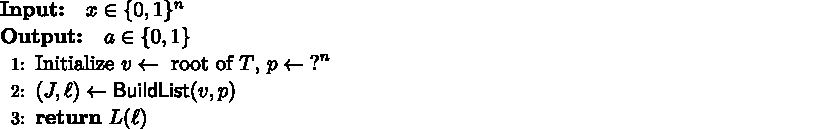
\includegraphics[width=\linewidth,height=0.78\textheight,keepaspectratio]{ccc2025-16-svg-07.pdf}\par






\par\medskip\noindent\textbf{
A.3 Direct sum for distribution-free discrepancy}\par



% SOURCE-ID Thmtheorem40


\par\medskip\noindent\textbf{
\textbf{Theorem 40}\textbf{.}
}\par



\emph{For every function $f\colon\{0,1\}^{n}\to\{0,1\}$ and $k\geq 1$,}\par


\[\begin{gathered}
k\cdot{\textup{disc}}(f)+1\geq{\textup{disc}}(f^{\oplus k})\geq k\cdot\big{(}{\textup{disc}}(f)-1\big{)}.
\end{gathered}\]



% END-SOURCE-ID Thmtheorem40



\par\medskip\noindent\textbf{Proof.}\par




The lower bound is a simple consequence of Lemma 8 by fixing $\mu$ to be a distribution such that ${\textup{disc}}(f)={\textup{disc}}(f,\mu)$ and observing that ${\textup{disc}}(f^{\oplus k})\geq{\textup{disc}}(f^{\oplus k},\mu^{k})$. The other direction is more interesting as it says that the hardest distribution for $f^{\oplus k}$ is basically $k$ products of the hardest distribution for a single copy $f$. Let $\|\widehat{f}\|_{\infty}^{*}\coloneqq\min_{\mu}\nobreak\ \|\widehat{F_{\mu}}\|_{\infty}$ where $\mu$ ranges over all distributions. Using Lemma 9, we obtain the following relation between ${\textup{disc}}(f)$ and $\|\widehat{f}\|_{\infty}^{*}$:\par


\[\begin{gathered}
-\log\|\widehat{f}\|_{\infty}^{*}+1\geq{\textup{disc}}(f)\geq-\log\|\widehat{f}\|_{\infty}^{*}.
\end{gathered}\]


Therefore, to prove the upper bound, it is enough to show a perfect direct product for $\|\widehat{f}\|_{\infty}^{*}$ and apply it $k$ time. To this end, fix some other function $g:\{0,1\}^{n}\to\{0,1\}$ and let us show that\par


\[\begin{gathered}
\|\widehat{f\oplus g}\|_{\infty}^{*}\geq\|\widehat{f}\|_{\infty}^{*}\cdot\|\widehat{g}\|_{\infty}^{*}.
\end{gathered}\]


Where we recall that $f\oplus g:\{0,1\}^{2n}\to\{0,1\}$. We can write $\|\widehat{f}\|_{\infty}^{*}$ as the value of the following linear program where the variables describe a distribution $\mu$:\par


\[\begin{gathered}
\emph{min.} \displaystyle\quad c \\
\emph{s.t.} \displaystyle\quad\Big{|}\sum\nolimits_{x\in\{0,1\}^{n}}(-1)^{f(x)}\cdot\mu_{x}\cdot(-1)^{\langle x,z\rangle}\Big{|}\leq c \displaystyle\quad\forall z\in\{0,1\}^{n} \\
\displaystyle\quad\sum\nolimits_{x\in\{0,1\}^{n}}\mu_{x}=1 \\
\displaystyle\quad\mu_{x}\geq 0 \displaystyle\quad\forall x\in\{0,1\}^{n}
\end{gathered}\]


The dual of (5) is:\par


\[\begin{gathered}
\emph{max.} \displaystyle\quad d \\
\emph{s.t.} \displaystyle\quad\sum\nolimits_{z\in\{0,1\}^{n}}(-1)^{f(x)}\cdot\beta_{z}\cdot(-1)^{\langle x,z\rangle}\geq d\quad\forall x\in\{0,1\}^{n} \\
\displaystyle\quad\sum\nolimits_{z\in\{0,1\}^{n}}|\beta_{z}|=1
\end{gathered}\]


Let $(\beta^{f},d^{f})$ and $(\beta^{g},d^{g})$ be the optimal feasible solutions to $(6)$ with respect to $f$ and $g$. By the strong duality theorem, it holds that $\|\widehat{f}\|_{\infty}^{*}=d^{f}$ and $\|\widehat{g}\|_{\infty}^{*}=d^{g}$. We now extract a feasible solution for (6) with respect to the function $f\oplus g$. Let $\beta\in\{0,1\}^{2n}$ be defined with $\beta_{(z_{1},z_{2})}=\beta^{f}_{z_{1}}\cdot\beta^{g}_{z_{2}}$ and observe that $(\beta,d^{f}\cdot d^{g})$ is a feasible solution for the dual of $\|\widehat{f\oplus g}\|_{\infty}^{*}$. By applying the strong duality theorem again, we have $\|\widehat{f\oplus g}\|_{\infty}^{*}\geq d^{f}\cdot d^{g}=\|\widehat{f}\|_{\infty}^{*}\cdot\|\widehat{g}\|_{\infty}^{*}$, as desired.
$\blacktriangleleft$\par






\par\medskip\noindent\textbf{
A.4 Some facts about parity decision trees}\par




Yao’s minimax principle is a powerful technique to analyse randomised algorithms – we adapt here the statement to parity trees, but the proof is exactly the same as the original one [55].\par



% SOURCE-ID Thmtheorem41


\par\medskip\noindent\textbf{
\textbf{Lemma 41}\textbf{.}
}\par



\emph{For any $f\colon\{0,1\}^{n}\to\{0,1\}$ and distribution $\mu$ over $\{0,1\}^{n}$, ${\textup{R}}_{\varepsilon}(f)\geq{\textup{D}}_{\varepsilon}(f,\mu)$.}\par



% END-SOURCE-ID Thmtheorem41



The following is a folklore fact relating randomised parity tree complexity and discrepancy [56, 3] which we re-prove in the parity context.\par



% SOURCE-ID Thmtheorem42


\par\medskip\noindent\textbf{
\textbf{Lemma 42}\textbf{.}
}\par



${\textup{D}}_{\varepsilon}(f,\mu)\geq{\textup{disc}}(f,\mu)+\log(1-2\varepsilon)$\emph{ for any $\varepsilon\in[0,1/2)$.}\par



% END-SOURCE-ID Thmtheorem42



\par\medskip\noindent\textbf{Proof.}\par




Fix a parity decision tree $T$ of depth $d\coloneqq{\textup{D}}_{\varepsilon}(f,\mu)$ which makes error $\mathrm{err}_{f}(T,\mu)\leq\varepsilon$, note that\par


\[\begin{gathered}
\displaystyle 1-2\varepsilon \displaystyle\leq\Pr_{\bm{x}\sim\mu}[T(\bm{x})=f(\bm{x})]-\Pr_{\bm{x}\sim\mu}[T(\bm{x})\neq f(\bm{x})] \\
\displaystyle=\sum\nolimits_{S\in\mathcal{L}}\Pr_{\bm{x}\sim\mu}[T(\bm{x})=f(\bm{x})\wedge\bm{x}\in S]-\Pr_{\bm{x}\sim\mu}[T(\bm{x})\neq f(\bm{x})\wedge\bm{x}\in S].
\end{gathered}\]


As $|\mathcal{L}(T)|\leq 2^{d}$, there exists some $S\in\mathcal{L}(T)$ – an affine subspace – with large correlation:\par


\[\begin{gathered}
{\textup{bias}}(f,\mu,S)=\left|\Pr_{\bm{x}\sim\mu}[T(\bm{x})=f(\bm{x})\wedge\bm{x}\in S]-\Pr_{\bm{x}\sim\mu}[T(\bm{x})\neq f(\bm{x})\wedge\bm{x}\in S]\right|\geq\frac{1-2\varepsilon}{2^{d}}.\
\end{gathered}\]


$\blacktriangleleft$
See 30\par





\par\medskip\noindent\textbf{Proof.}\par




Let ${\textrm{\small{NOR}}}_{n}:\{0,1\}^{n}\to\{0,1\}$ be the function that checks whether the input is $0^{n}$ and rejects otherwise. Observe that one iteration of the sumcheck protocol can be performed in one parity query. More precisely for any $x\in\{0,1\}^{n}$, if $\bm{s}\sim U\left(\{0,1\}^{n}\right)$ then:\par


\[\begin{gathered}
\Pr_{\bm{s}}[\langle x,\bm{s}\rangle=1]=\begin{cases}1/2&\quad\text{if $x\neq 0^{n}$}\\
0&\quad\text{if $x=0^{n}$}\end{cases}.
\end{gathered}\]


Performing two random checks independently shows that ${\textup{R}}({\textrm{\small{NOR}}}_{n},1/4)\leq O(1)$. It is a folklore result that a (classical) randomised decision tree can solve ${\textrm{\small{FFO}}}_{n}$ with probability $\varepsilon$ using $O(\log n+\log(1/\varepsilon))$ oracle NOR-queries even if the oracle fails with probability $1/3$ [24, 44]. We highlight that this is an improvement over the naive method that boosts the noisy NOR queries and yields complexity $O(\log(n)^{2}\log(1/\varepsilon))$. Recent work [30, §3] revisits this trick in depth for communication complexity and their result can be re-interpreted in the context of parity decision trees as follows:\par


\[\begin{gathered}
\forall f\colon\,{\textup{R}}(f,\varepsilon)\leq O\big{(}{\textup{D}}^{{\textrm{\small{\scriptsize NOR}}}}(f)+\log(1/\varepsilon)\big{)}.
\end{gathered}\]


Thus, plugging in $f={\textrm{\small{FFO}}}$ and noting that ${\textup{D}}^{{\textrm{\small{\scriptsize NOR}}}}({\textrm{\small{FFO}}}_{n})\leq\log n$ (with binary search), we get the desired result.
$\blacktriangleleft$
See 11\par





\par\medskip\noindent\textbf{
\textbf{Proof}.}\par




Let $\mathcal{T}$ be a randomised PDT satisfying that $d\coloneqq\overline{q}(\mathcal{T},\mu)=\overline{{\textup{D}}}_{\varepsilon}(f,\mu)$ and $\mathrm{err}_{f}(\mathcal{T},\mu)\leq\varepsilon$.
To prove the lemma, it suffices to construct a deterministic parity tree $T$ of depth $T\leq d/\gamma$ with $\mathrm{err}_{f}(T,\mu)\leq\varepsilon+\gamma$. Sample $\bm{T}\sim\mathcal{T}$. We construct a new tree $\bm{T}^{\prime}$ by pruning $\bm{T}$ as follows: We remove all the nodes of $\bm{T}$ of depth greater than $d/\delta$. If any node of depth $d/\delta$ becomes a leaf, we label it with an arbitrary bit. Note that $\bm{T}^{\prime}$ has depth $\leq d/\delta$. Finally, let $\mathcal{T}^{\prime}$ denote the distribution over $\bm{T}^{\prime}$ inherited from $\mathcal{T}$.\par




We observe that for each $x\in\{0,1\}^{n}$, both $\bm{T}(x)=f(x)$ and $\bm{T}^{\prime}(x)\neq f(x)$ happen only if $q(\bm{T},x)>d/\gamma$. Moreover, by Markov’s inequality,\par


\[\begin{gathered}
\Pr\nolimits_{\begin{subarray}{c}\bm{T}\sim\mathcal{T}\\
\bm{x}\sim\mu\end{subarray}}[q(\bm{T},\bm{x})>d/\gamma]\leq\frac{\overline{q}(\bm{T},\mu)}{d/\gamma}=\gamma.
\end{gathered}\]


Therefore, $\mathrm{err}_{f}(\mathcal{T}^{\prime},\mu)\leq\mathrm{err}_{f}(\mathcal{T},\mu)+\gamma\leq\varepsilon+\gamma$. By an averaging argument, there exists some $T\in\mathrm{supp}(\mathcal{T}^{\prime})$ of depth $\leq d/\delta$ that computes $f$ with error $\mathrm{err}_{f}(T,\mu)\leq\varepsilon+\gamma$, as desired.
$\vartriangleleft$\par






\par\medskip\noindent\textbf{
A.5 Omitted proofs of Section 6
}\par




In this appendix, we prove Claim 29, an alternative description for the distributions of Section 6.1. Let $p^{1},p^{2}\in\{0,\star,\mathord{?}\}^{n}$. We write $p^{1}\sim p^{2}$ if $p^{1}$ and $p^{2}$ are consistent over their non$-\mathord{?}$ entries. That is, $p^{1}\sim p^{2}$ if for all $j\in[n]$, if $p^{1}_{j}\neq\mathord{?}$ and $p^{2}_{j}\neq\mathord{?}$, then $p^{1}_{j}=p^{2}_{j}$. Claim 29 follows from Claims 43 and 44.\par



% SOURCE-ID Thmtheorem43


\par\medskip\noindent\textbf{
Claim 43. 
}\par



For every reachable state $(v,p)$, consistent $x\in\{0,1\}^{n}$ and $\rho\in\{0,\star\}^{n}$, $\mathcal{R}^{v,p,x}\equiv\widehat{\mathcal{R}}^{p,x}$.\par



% END-SOURCE-ID Thmtheorem43



\par\medskip\noindent\textbf{
\textbf{Proof}.}\par




Upon inspection of $\widehat{\mathcal{R}}^{v,p}$, it is enough to prove that for all $x\in\{0,1\}^{n}$:\par


\[\begin{gathered}
\Pr_{\bm{\rho}\sim\mathcal{R}^{v,p,x}}[\bm{\rho}=\rho]=\prod_{j\in S^{p}_{\neq\mathord{?}}}\mathbbm{1}\left[\rho_{j}=p_{j}\right]\times\prod\nolimits_{\begin{subarray}{c}j\in S^{p}_{\mathord{?}}\\
x_{j}=1\end{subarray}}\mathbbm{1}\left[\rho_{j}=\star\right]\times\prod\nolimits_{\begin{subarray}{c}j\in S^{p}_{\mathord{?}}\\
x_{j}=0\end{subarray}}\begin{cases}\delta_{j}/(2-\delta_{j})&\textup{if $\rho_{j}=\star$}\\
1-\delta_{j}/(2-\delta_{j})&\textup{if $\rho_{j}=0$}\end{cases}.
\end{gathered}\]


Fix $x\in\{0,1\}^{n}$. We prove this by induction on the state space $(v,p)$ consistent with $x$. The entry-point of the state space is $(\textup{root}(T),\mathord{?}^{n})$. In this case, the statement holds by definition. Suppose now that the statement is true for state $(v,p)$. Depending on the value of $\rho$, there are several next state $(v^{\prime},p^{\prime})$ possible. Observe however that the next vertex of $T$ to be visited does not depend on $\rho$, as it is fixed to be $v^{\prime}\coloneqq\mathrm{child}(v,\langle x,Q^{v}\rangle)$. For any fixed $\rho\in\{0,\star\}^{n}$, we have:\par


\[\begin{gathered}
\displaystyle\Pr\nolimits_{\bm{\rho}\sim\mathcal{R}^{v^{\prime},p^{\prime},x}}[\bm{\rho}=\rho] \displaystyle=\Pr\nolimits_{\bm{x}\sim\mu,\bm{\rho}\sim R_{\mu}^{\bm{x}}}[\bm{\rho}=\rho\mid\textup{$(v^{\prime},p^{\prime})$ is reached and $\bm{x}=x$}] \\
\displaystyle=\frac{\Pr_{\bm{x},\bm{\rho}}[\textup{$\bm{\rho}=\rho$ and $(v^{\prime},p^{\prime})$ is reached and $\bm{x}=x$}]}{\Pr_{\bm{x},\bm{\rho}}[\textup{$(v^{\prime},p^{\prime})$ is reached and $\bm{x}=x$}]}.
\end{gathered}\]


Note that there can be only one state from which $(v^{\prime},p^{\prime})$ can be reached, namely $(v,p)$. Indeed, suppose that there is another state $(v,p^{\star})$ from which $(v^{\prime},p^{\prime})$ can be reached. Then $(v,p)$ and $(v,p^{*})$ have a common ancestor $(u,q)$. Since the paths diverged after $(u,q)$, it must be that $p\nsim p^{*}$ and thus $p^{*}\nsim p^{\prime}$: a contradiction. Thus, we have the following equivalence:\par


\[\begin{gathered}
\textup{$(v^{\prime},p^{\prime})$ is reached}\quad\iff\quad\textup{$(v,p)$ is reached and $\rho\sim p^{\prime}$}.
\end{gathered}\]


Therefore, we have:\par


\[\begin{gathered}
\Pr\nolimits_{\bm{\rho}\sim\mathcal{R}^{v^{\prime},p^{\prime},x}}[\bm{\rho}=\rho]=\frac{\Pr_{\bm{\rho}\sim\mathcal{R}^{v,p,x}}[\bm{\rho}=\rho]\cdot\mathbbm{1}\left[\rho\sim p^{\prime}\right]}{\Pr_{\bm{\rho}\sim\mathcal{R}^{v,p,x}}[\bm{\rho}\sim p^{\prime}]}.
\end{gathered}\]


We can now use the inductive hypothesis on $(v,p)$. Since $\rho\sim p^{\prime}$ implies $\rho\sim p$, the numerator of  7 simplifies to:\par


\[\begin{gathered}
\prod\nolimits_{j\in S^{p^{\prime}}_{\neq\mathord{?}}}\mathbbm{1}\left[\rho_{j}=p_{j}\right]\times\prod\nolimits_{\begin{subarray}{c}j\in S^{p}_{\mathord{?}}\\
x_{j}=1\end{subarray}}\mathbbm{1}\left[\rho_{j}=\star\right]\times\prod\nolimits_{\begin{subarray}{c}j\in S^{p}_{\mathord{?}}\\
x_{j}=0\end{subarray}}\begin{cases}\delta_{j}/(2-\delta_{j})&\textup{if $\rho_{j}=\star$}\\
1-\delta_{j}/(2-\delta_{j})&\textup{if $\rho_{j}=0$}\end{cases}.
\end{gathered}\]


Let $\Delta=S^{p}_{\mathord{?}}\setminus S^{p^{\prime}}_{\mathord{?}}$ and observe that the denominator of  7 is equal to:\par


\[\begin{gathered}
\prod\nolimits_{\begin{subarray}{c}j\in\Delta\\
x_{j}=1\end{subarray}}\mathbbm{1}\left[\rho_{j}=\star\right]\times\prod\nolimits_{\begin{subarray}{c}j\in\Delta\\
x_{j}=0\end{subarray}}\begin{cases}\delta_{j}/(2-\delta_{j})&\textup{if $\rho_{j}=\star$}\\
1-\delta_{j}/(2-\delta_{j})&\textup{if $\rho_{j}=0$}\end{cases}.\
\end{gathered}\]


$\vartriangleleft$\par



% SOURCE-ID Thmtheorem44


\par\medskip\noindent\textbf{
Claim 44. 
}\par



For every reachable state $(v,p)$ and $x\in\{0,1\}^{n}$, $\mathcal{X}^{v,p}\equiv\widehat{\mathcal{X}}^{v,p}$.\par



% END-SOURCE-ID Thmtheorem44




\par\medskip\noindent\textbf{
\textbf{Proof}.}\par




Fix some $(v,p)$ and $x\in\{0,1\}^{n}$. Upon inspection of $\widehat{X}^{v,p}$, it is enough to prove that\par


\[\begin{gathered}
\Pr\nolimits_{\bm{x}\sim\mathcal{X}^{v,p}}[\bm{x}=x]=M(x,v,p)\cdot\prod\nolimits_{j\in S^{p}_{?}}1-\delta_{j}/2-x_{j}\cdot(1-\delta_{j}),
\end{gathered}\]


where $M(x,v,p)$ is an indicator set to 1 if and only if for all $j\in[n]$, $p_{j}=0$ implies $x_{j}=0$ and $\langle x,Q^{u}\rangle=b^{u}$ for all $u\in\mathrm{path}(v)$.
By Baye’s rule we have:\par


\[\begin{gathered}
\Pr_{\bm{x}\sim\mathcal{X}^{v,p}}[\bm{x}=x]=\Pr\nolimits_{\begin{subarray}{c}\bm{x}\sim\mu\\
\bm{\rho}\sim\mathcal{R}_{\mu}^{\bm{x}}\end{subarray}}[\bm{x}=x\mid\text{$(v,p)$ is reached on $(\bm{x},\bm{\rho})$}]=\frac{p(x)}{\sum_{x^{\prime}\in\{0,1\}^{n}}p(x^{\prime})},
\end{gathered}\]


where\par


\[\begin{gathered}
p(x)\coloneqq\Pr_{\bm{x},\bm{\rho}}[\bm{x}=x]\cdot\Pr_{\bm{x},\bm{\rho}}[\text{$(v,p)$ is reached on $(\bm{x},\bm{\rho})$}\mid\bm{x}=x].
\end{gathered}\]


To analyse $p(x)$, we have:\par


\[\begin{gathered}
\Pr\nolimits_{\begin{subarray}{c}\bm{x}\sim\mu\\
\bm{\rho}\sim\mathcal{R}_{\mu}^{\bm{x}}\end{subarray}}[\bm{x}=x]=\Pr\nolimits_{\bm{x}\sim\mu}[\bm{x}=x]=\prod\nolimits_{j\in[n]}\Pr_{\bm{x}\sim\mu}[\bm{x}_{j}=x_{j}]=\prod\nolimits_{j\in[n]}1-(\delta_{j}/2)-x_{j}\cdot(1-\delta_{j}).
\end{gathered}\]


On the other hand, the second component of $p(x)$ is clearly zero if $M(x,v,p)=0$. For instance, $v$ cannot be reached if $x$ does not satisfy all equations on the path to $v$. Thus, we have:\par


\[\begin{gathered}
\displaystyle\Pr\nolimits_{\begin{subarray}{c}\bm{x}\sim\mu\\
\bm{\rho}\sim\mathcal{R}_{\mu}^{\bm{x}}\end{subarray}}[\text{$(v,p)$ is reached on $(\bm{x},\bm{\rho})$}\mid\bm{x}=x] \\
\displaystyle= \displaystyle\Pr\nolimits_{\bm{\rho}\sim\mathcal{R}_{\mu}^{x}}[\text{$(v,p)$ is reached on $(x,\bm{\rho})$}] \\
\displaystyle= \displaystyle M(x,v,p)\cdot\Pr\nolimits_{\bm{\rho}\sim\mathcal{R}_{\mu}^{x}}[\bm{\rho}\sim p] \\
\displaystyle= \displaystyle M(x,v,p)\cdot\prod\nolimits_{j\in S^{p}_{0}}\frac{2-2\delta_{j}}{2-\delta_{j}}\cdot\prod\nolimits_{j\in S^{p}_{\star}}\left(\frac{\delta_{j}}{2-\delta_{j}}\right)^{1-x_{j}}.
\end{gathered}\]


Combining those two observations, we get:\par


\[\begin{gathered}
p(x)=M(v,p,x)\cdot\prod\nolimits_{j\in S^{p}_{?}}\big{(}1-\delta_{j}/2-x_{j}\cdot(1-\delta_{j})\big{)}\cdot\prod\nolimits_{j\in S^{p}_{0}}(1-\delta_{j})\cdot\prod\nolimits_{j\in S^{p}_{\star}}\delta_{j}/2.
\end{gathered}\]


Observe that the last two products do not involve $x$ at all and can thus be cancelled in the initial expression:\par


\[\begin{gathered}
\displaystyle\Pr_{\bm{x}\sim\mathcal{X}^{v,p}}[\bm{x}=x] \displaystyle=\frac{p^{\prime}(x)}{\sum_{x^{\prime}}p^{\prime}(x)}\text{ where }p^{\prime}(x)=M(x,v,p)\cdot\prod\nolimits_{j\in S^{p}_{?}}\big{(}1-\delta_{j}/2-x_{j}\cdot(1-\delta_{j})\big{)}.
\end{gathered}\]


Finally, observe that $M(x,v,p)$ fixes the value of all the bits of $x$ except for $S^{p}_{?}$. Thus, the summation in the denominator equals 1 and the claim follows.
$\vartriangleleft$\par




\par





\end{document}
